\documentclass[9pt,twoside,lineno]{pnas-new}
% Use the lineno option to display guide line numbers if required.

%\pdfoutput=1
\usepackage{amsmath}

%----------------------------------------------------------------------------------------%

\usepackage{amsfonts}
\usepackage{amssymb}
\usepackage{amsthm}

\usepackage{graphicx}
\usepackage{hyperref}

%\usepackage[left=1.25in,right=1.25in,top=1.5in,bottom=1.25in]{geometry}

\usepackage{multirow}

\usepackage{verbatim}
\usepackage{float}
\usepackage{rotating}
\usepackage{pxfonts}
\usepackage{isomath}

\usepackage{newpxtext}
\usepackage{newpxmath}
\usepackage{xcolor}
%\usepackage[dvipsnames]{xcolor}
\usepackage[normalem]{ulem}
\usepackage{booktabs}
\usepackage{tikz}


% packages for rmd output
\usepackage{tabu}
\providecommand{\tightlist}{%
  \setlength{\itemsep}{0pt}\setlength{\parskip}{0pt}}
\usepackage{float}
\usepackage{booktabs}

\usepackage{subcaption}

\newtheorem{theorem}{Theorem}[section]
\newtheorem{conjecture}{Conjecture}[section]
\newtheorem{corollary}{Corollary}[section]
\newtheorem{lemma}{Lemma}[section]
\newtheorem{proposition}{Proposition}[section]
\theoremstyle{definition}
\newtheorem{assumption}{}[section]
\renewcommand{\theassumption}{A\arabic{assumption}}
\newtheorem{definition}{Definition}[section]
\newtheorem{step}{Step}[section]
\newtheorem{remark}{Comment}[section]
\newtheorem{example}{Example}[section]
\newtheorem*{example*}{Example}
\newtheorem{mpart}{Part}
\newtheorem{problem}{Problem}

\usepackage{calc,tikz,nicefrac}

\usepackage[section]{placeins}

\usetikzlibrary{positioning}
\geometry{letterpaper}
%\usepackag\Ep[parfill]{parskip}    % Activate to begin paragraphs
%with an empty line rather than an indent

\setlength{\parskip}{.4cm}
\geometry{centering}
\usepackage{mathtools}

\usepackage{bm}

%\usepackage[authoryear]{natbib}

%\usepackage{pdflscape}

\usepackage{afterpage}
\usepackage{capt-of}



\newcommand{\argmax}{\operatornamewithlimits{arg\,max}}
\newcommand{\argmin}{\operatornamewithlimits{arg\,min}}
\def\inprobLOW{\rightarrow_p}
\def\inprobHIGH{\,{\buildrel p \over \rightarrow}\,}
\def\inprob{\,{\inprobHIGH}\,}
\def\indist{\,{\buildrel d \over \rightarrow}\,}
\def\F{\mathbb{F}}
\newcommand{\gmatrix}[1]{\begin{pmatrix} {#1}_{11} & \cdots &
    {#1}_{1n} \\ \vdots & \ddots & \vdots \\ {#1}_{m1} & \cdots &
    {#1}_{mn} \end{pmatrix}}
\newcommand{\iprod}[2]{\left\langle {#1} , {#2} \right\rangle}
\newcommand{\norm}[1]{\left\Vert {#1} \right\Vert}
\newcommand{\abs}[1]{\left\vert {#1} \right\vert}
\renewcommand{\det}{\mathrm{det}}
\newcommand{\rank}{\mathrm{rank}}
\newcommand{\spn}{\mathrm{span}}
\newcommand{\row}{\mathrm{Row}}
\newcommand{\col}{\mathrm{Col}}
\renewcommand{\dim}{\mathrm{dim}}
\newcommand{\prefeq}{\succeq}
\newcommand{\pref}{\succ}
\newcommand{\seq}[1]{\{{#1}_n \}_{n=1}^\infty }
\renewcommand{\to}{{\rightarrow}}
\providecommand{\Infected}{{\mathcal{I}}}
\providecommand{\Recovered}{{R}}

\providecommand{\Er}{{\mathrm{E}}}
\providecommand{\Var}{{\mathrm{Var}}}
\providecommand{\set}[1]{\left\{#1\right\}}
\providecommand{\plim}{\operatornamewithlimits{plim}}
\newcommand\indep{\protect\mathpalette{\protect\independenT}{\perp}}
\def\independenT#1#2{\mathrel{\setbox0\hbox{$#1#2$}%
    \copy0\kern-\wd0\mkern4mu\box0}}

\newcommand{\ad}{\overset{\mathrm{a}}{\sim}}
\newcommand{\Z}{\mathbb{Z}}
\newcommand{\R}{\mathbb{R}}
%\renewcommand{\C}{\mathbb{C}}
\newcommand{\N}{\mathbb{N}}
\newcommand{\mS}{\mathcal{S}}
\newcommand{\mF}{\mathcal{F}}
\newcommand{\mE}{\mathcal{E}}
\newcommand{\mG}{\mathcal{G}}
\newcommand{\mL}{\mathcal{L}}
\renewcommand{\qed}{\hfill{\tiny \ensuremath{\blacksquare} }}%

\newcommand{\Ep}{{\mathrm{E}}}
\newcommand{\barEp}{\bar \Ep}
\newcommand{\En}{{\mathbb{E}_n}}
\renewcommand{\Pr}{{\mathrm{P}}}

%\newcommand{\mathbbeta}{\mbox{$\beta$}}
%\newcommand{\btheta}{\mbox{$\theta$}}
%\newcommand{\bdelta}{\mbox{$\delta$}}
\newcommand{\balpha}{\mbox{$\alpha$}}
\newcommand{\stheta}{\mbox{\scriptsize \theta}}

\renewcommand{\indep}{\perp \!\!\! \perp}
\newcommand{\mC}{\mathcal{C}}
\newcommand{\mU}{\mathcal{U}}
\newcommand{\mX}{\mathcal{X}}
\newcommand{\mJ}{\mathcal{J}}
\newcommand{\df}{\mathrm{df}}
\newcommand{\bP}{\mathbb{P}}
\newcommand{\bE}{\mathbb{E}}
\newcommand{\bEn}{\mathbb{E}_{n}}
\newcommand{\bG}{\mathbb{G}}

\newcommand{\eps}{\varepsilon}

%
%\usepackage{xr}
%\externaldocument{COVID-school}

\usepackage{neuralnetwork}

\def\bcolor{\color{brown}}
\def\pcolor{\color{blue}}
\def\icolor{\color{magenta}}
\def\wcolor{\color{gray}}
\def\ycolor{\color{red}}
\usepackage{CJKutf8}


\DeclareMathOperator{\dist}{dist} % The distance.

\templatetype{pnassupportinginfo}

\title{The Association of Opening K-12 Schools with the Spread of COVID-19 in the United States: County-Level Panel Data Analysis}
\author{Victor Chernozhukov, Hiroyuki Kasahara, and Paul Schrimpf}

 

\correspondingauthor{Hiroyuki Kasahara  \begin{CJK}{UTF8}{goth}(笠原博幸)\end{CJK}\\E-mail: hkasahar@mail.ubc.ca}

\begin{document}

%% Comment out or remove this line before generating final copy for submission; this will also remove the warning re: "Consecutive odd pages found".
%\instructionspage  

\maketitle

%% Adds the main heading for the SI text. Comment out this line if you do not have any supporting information text.
%\SItext
 
 

\subsection*{The Model and Methods}\label{sec:causal-mode-SI}

\subsubsection*{The Structural Causal Model}
Our approach draws on the framework presented in our previous paper \cite{chernozhukov2021}. Here we summarize the approach 
for completeness, highlighting the main difference  (here we do not assume that all relevant social distancing behavioral variables are observed).

We begin with a qualitative description of the model via a causal path diagram shown in Figure \ref{Wright}, which describes how policies, behavior, and information interact together:
\begin{itemize}
\item The \textit{forward} health outcome,
$Y_{i,t+\ell}$, is determined last, after all other variables have been determined;
\item The  adopted vector of policies, $P_{it}$,  affect health outcome $Y_{i,t+\ell}$ either directly, or indirectly by altering  individual distancing and other precautioanry behavior  $B_{it}$, which may be only partially observed;
\item  Information variables, $I_{it}$, such as lagged values of outcomes and other lagged observable variables (see robustness checks) can affect human behavior and  policies, as well as  outcomes;
\item The confounding factors $W_{it}$, which vary across counties and time, affect all other variables; these include
unobserved though estimable county, time, state, state-week effects.
\end{itemize}
The index $i$ denotes observational unit, the county, and $t$ and $t+\ell$ denotes the time, where  $\ell$ represents the typical time lag  between infection and case confirmation or death.
\begin{figure}[ht]
\begin{center}
\begin {tikzpicture}[-latex, auto, node distance =2cm and 3.5cm, on grid, thick,
  empty/.style ={circle, top color=white, bottom color = white, draw, white, text=white , minimum width =1.25 cm},
  policy/.style ={circle, top color=white, bottom color = blue, draw, black, text=black , minimum width =1.25 cm},
%    behavior/.style ={circle, top color=white, bottom color = brown, draw, dashed, black, text=black , minimum width =1.25 cm},
    behavior/.style ={circle, top color=white, bottom color = brown, draw, black, text=black , minimum width =1.25 cm},
   observed/.style ={circle, top color=white, bottom color = magenta, draw, black, text=black , minimum width =1.25 cm} ,
   confounder/.style ={circle, top color=white, bottom color =  gray, draw, black, text=black , minimum width =1.25 cm} ,
outcome/.style ={circle, top color=white, bottom color = red, draw, black, text=black , minimum width =1.25 cm} ]

\node[policy]   (P) {\tiny $P_{it}$};
\node[empty] (E) [below=of P] {\tiny $I_{it}$};
\node[outcome]  (Y) [right =of E] {\tiny $Y_{i,t+\ell}$};
\node[behavior] (B) [below =of E] {\tiny $B_{it}$};
\node[observed] (I) [left =of P] {\tiny $I_{it}$};
\node[confounder] (W) [left=of B] {\tiny  $W_{it}$};
\path[->] (P) edge (Y);
\path[->] (B) edge (Y);
\path[->] (P) edge (B);
\path[->] (I) edge (B);
\path[->] (I) edge (P);
\path[->] (W) edge (Y);
\path[->] (W) edge (B);
\path[->] (W) edge (P);
\path[->] (W) edge (I);
\path[->] (I) edge (Y);

\end{tikzpicture} \end{center}
\caption{The causal path diagram for our model.}\label{Wright}
\end{figure}

Our main outcomes of interest are the growth rates in Covid-19 cases and deaths and policy variables include school reopening in various modes, mask mandates, ban gathering, and stay-at-home orders,  and the information variables include lagged values of outcome (as well as other variables described in the sensitivity checks). %We provide a detailed description of these variables and their timing in Section TBD.   


The role of behavioral variables in the model is two-fold. First, the presence of these variables in the model requires us to control for the information variables -- even when information variables affect outcomes only through policies or behavior.  In this case conditioning on the information blocks the backdoor path (see, \cite{pearl:causality}) creating confounding $${\ycolor Y_{i,t+\ell}} \longleftarrow {\bcolor B_{it}} \longleftarrow  {\icolor I_{it}} \longrightarrow {\pcolor P_{it}}.$$  Therefore conditioning on the information is important even when there is no direct effect  ${\icolor I_{it}} \longrightarrow {\ycolor Y_{i,t+\ell}}$. This observation motivates our main dynamic specification below, where information variables include lagged growth rates and new cases or new deaths per capita. Second, while not all behavioral variables may be observable, we can still study as the matter of supporting analysis, the effects of policies on observed behavioral variables (the portion of time in workplace, restaurants, and bars) and of behavioral variables on outcomes, thereby gaining insight as to whether policies have changed private behavior and to what extent this private behavior changed the outcomes  (for the analysis, of early pandemic data in this vein, see our previous paper).

The causal structure allows for the effect of the policy to be either direct or indirect. The structure also allows for changes in behavior to be brought by the change in policies and information. These are all realistic properties that we expect from the context of the problem. Policies such as closures and reopenings of schools, closures or reopening of non-essential business, and restaurants, affect the behavior in strong ways.  In contrast, policies such as mandating employees to wear masks can potentially affect the Covid-19 transmission directly.  The information variables, such as recent growth in the number of cases, can cause people to spend more time at home, regardless of adopted policies; these changes in
behavior, in turn, affect the transmission of Covid-19.

The causal ordering induced by this directed acyclical graph is determined by the following
timing sequence: % \textit{within a period}:%\footnote{Mathematically this corresponds to the factorization of the data likelihood, omitting indexes, $$f_{Y,P,B, I, W} = f_{Y\mid P, B,I, W} f_{B \mid P,I,W } f_{P \mid I, W} f_{I,W}.$$ }
\begin{itemize}
\item[(1)]  information and confounders get determined at $t$,
\item[(2)] policies are set in place, given information and confounders at $t$;
\item[(3)] behavior is realized, given policies, information, and confounders at $t$;
\item[(4)] outcomes get realized at $t+\ell$ given policies, behavior, information, and confounders.
\end{itemize}

The model also allows for direct dynamic effects of information variables on the outcome through autoregressive structures that capture persistence in growth patterns. We do not highlight these dynamic effects and only study the short-term effects (longer-run effects get typically amplified; see our previous paper \cite{chernozhukov2021} for more details.)

Our quantitative model for causal structure in Figure \ref{Wright} is given by the following econometric structural equation model:\begin{equation} \label{eqn:SEM1} \tag{SEM}
  \begin{aligned}
   &  {\ycolor Y_{i,t+\ell}} (b,p,\iota) &:=& {\bcolor \alpha ' b}  +  {\pcolor \pi 'p} +
    {\icolor \mu'\iota } + {\wcolor \delta_Y 'W_{it}} + \varepsilon^y_{it}, \\
   &  {\bcolor B_{it}} (p,\iota) &:= & {\pcolor \beta'p } + {\icolor \gamma'\iota} +      {\wcolor\delta_B 'W_{it} } + \varepsilon^b_{it}, \\
   & {\pcolor P_{it}}   (\iota) & := &  p ({\icolor \eta'\iota}, {\wcolor W_{it}},  \varepsilon^p_{it} ), 
         \end{aligned}
 \end{equation}
which is a collection of structural potential response functions (potential outcomes), where the stochastic schocks
are decomposed into an observable part $\delta' W$ and unobservable part $\varepsilon$.  Lower case letters
$\iota$, $b$ and $p$ denote the potential values of information, behavior, and policy variables. The restrictions on shocks are described below. 

The observed outcomes, policy, and behavior variables are generated by setting $\iota= {\icolor I_{it}}$ and propagating
the system from the last equation to the first:
%\begin{equation} \label{eqn:SEM2}
\[
  \begin{aligned}
& {\ycolor Y_{i,t+\ell}}  & := & Y_{i,t+\ell} ( {\bcolor B_{it} } ,{\pcolor P_{it}}, {\icolor I_{it}}), \\
& {\bcolor B_{it} } & := &   B_{it}({\pcolor P_{it} } ,{\icolor I_{it}}), \\
& {\pcolor P_{it} }& := &  P_{it}({\icolor I_{it}}). \end{aligned}
\]


The orthogonality restrictions on the stochastic components are as follows: The stochastic shocks $\varepsilon^y_{it}$
and  $\varepsilon^p_{it}$ are centered and furthermore,
\begin{equation}\label{eqn:SEM2} \tag{O}
\begin{aligned}
   & \varepsilon^y_{it} &  \perp &  \quad (\varepsilon^b_{it}, P_{it}, {\wcolor W_{it}}, {\icolor I_{it}}), \\
&  \varepsilon^b_{it}  & \perp & \quad  (P_{it}, {\wcolor W_{it}}, {\icolor I_{it}}), \\
&   \varepsilon^p_{it} &  \indep &  \quad ({\wcolor W_{it}}, {\icolor I_{it}}),
\end{aligned}
\end{equation}
where we say that $V \perp U$ if $\Ep VU = 0$. This is a standard way of representing restrictions on errors in structural equation modeling. The last equation states that variation in policies is exogenous conditionally on confounders and information variables.

%\footnote{ An alternative useful
%starting point is to impose the Rubin-Rosenbaum type unconfoudedness condition:
%$$
%Y_{i,t+\ell} (\cdot,\cdot,\cdot)  \indep (P_{it}, B_{it}, I_{it})  \mid W_{it}, \
%B_{it} (\cdot,\cdot)  \indep (P_{it}, I_{it})  \mid W_{it}, \
% P_{it} (\cdot)  \indep  I_{it}  \mid W_{it},
%$$
%which imply, with treating stochastic errors as independent additive components, the orthogonal conditions stated above.
% }%\footnote{The structural equations of this form are connected to triangular structural equation models, appearing
 %in microeconometrics and macroeconometrics (SVARs), going back to the work of  \cite{strotz1960recursive}. .}

The system above together with  orthogonality restrictions (\ref{eqn:SEM2}) implies the following collection of stochastic equations for realized variables:
\begin{align}
   &  {\ycolor  Y_{i,t+\ell}}
    = {\bcolor\alpha ' B_{it}} + {\pcolor\pi 'P_{it}} + {\icolor\mu'I_{it}} + {\wcolor\delta_Y 'W_{it}}  + \varepsilon^y_{it},
    &  & \varepsilon^y_{it} \perp {\bcolor B_{it}}, {\pcolor P_{it}}, {\icolor I_{it}}, {\wcolor W_{it}} \label{eq:R1} \tag{BPI$\to$Y} \\
    &  {\bcolor B_{it}}
     =  {\pcolor \beta' P_{it}} + {\icolor \gamma'I_{it}} +  {\wcolor \delta_B' W_{it}} + \varepsilon^b_{it},
   & & \varepsilon^b_{it} \perp {\pcolor P_{it}}, {\icolor I_{it}}, {\wcolor W_{it}}  \label{eq:R2} \tag{PI$\to$B} 
         \end{align}

As discussed below, the information variable includes case growth. Therefore, the orthogonality restriction  $ \varepsilon^y_{it} \perp   {\pcolor P_{it}}$ holds if  the government does not have knowledge on future case growth beyond what is predicted by the information set and the  confounders; even when the government has some knowledge on $\varepsilon^y_{it}$, the orthogonality restriction may hold if there is a time lag for the government to implement its policies based on $\varepsilon^y_{it}$.

We stress that our  main analysis does not require all components of ${\bcolor B_{it}}$ to be observable. 

\textbf{Main Implication.} The model stated above implies the following projection equation:

\begin{align}
   {\ycolor  Y_{i,t+\ell}}
   =    a'  {\pcolor P_{it}} +b'  {\icolor I_{it} }+ c' {\wcolor W_{it}}  + {\bar \varepsilon}_{it},  \quad   {\bar \varepsilon}_{it} \perp
  {\pcolor P_{it}},  {\icolor I_{it}}, {\wcolor W_{it}},  \label{eq:R4} \tag{PI$\to$Y}
     \end{align}
where 
$$
a' := ( {\bcolor\alpha '}  {\pcolor \beta' }+{\pcolor\pi'} ), \quad b' := ( {\bcolor\alpha '}  {\icolor \gamma'} + {\icolor \mu'}),
\quad c' :=  ( {\bcolor\alpha '}  {\wcolor \delta_B' }+{\wcolor\delta_Y'} )
$$
This follows immediately from plugging equation (PI $\to$ B) to  equation (BPI $\to$ Y) and verifying
that the composite stochastic shock $\bar \varepsilon_{it}$ obeys the orthogonality condition stated 
in  (\ref{eq:R4}).


The main parameter of interest is the structural causal effect of the policy:
$$
a' = ( {\bcolor\alpha '}  {\pcolor \beta' }+{\pcolor\pi'} ).
$$
It comprises direct policy effect ${\pcolor\pi'}$ as well as the indirect effect $ {\bcolor\alpha '}  {\pcolor \beta' }$, realized by 
the policy changing observed and unobserved behavior variables ${\bcolor B_{it}}$.   This coefficient $a$ and $b$ can estimated directly using the dynamic panel data methods described in more detail below.  


As additional analysis, we can estimate the determinants for the observed behavioral mobility measures-- the observed part of  ${\bcolor B_{it}}$. 


%The orthogonality condition in (\ref{eq:R4}) is weaker than the orthogonality conditions in  (\ref{eq:R1})-(\ref{eq:R2}) in that the former is implied by the latter but not vice versa.
%The system over-identifies the regression coefficients because  $({\bcolor\alpha '}  {\pcolor \beta' }+{\pcolor\pi'})$ and $({\bcolor\alpha '}  {\icolor \gamma'} + {\icolor \mu'})$ in  (\ref{eq:R4}) can be also identified from  ${\bcolor\alpha ' }$,  $ {\pcolor\pi '}$, ${\icolor\mu'}$,   ${\pcolor \beta' }$, and ${\icolor \gamma'}$ in (\ref{eq:R1})-(\ref{eq:R2}).  Comparing the estimates of $({\bcolor\alpha '}  {\pcolor \beta' }+{\pcolor\pi'})$ and $({\bcolor\alpha '}  {\icolor \gamma'} + {\icolor \mu'})$ from  (\ref{eq:R4})  with  those implied by  the estimates of ${\bcolor\alpha ' }$,  $ {\pcolor\pi '}$, ${\icolor\mu'}$,   ${\pcolor \beta' }$, and ${\icolor \gamma'}$ from   (\ref{eq:R1})-(\ref{eq:R2}) provides a useful specification test.


\subsubsection*{Identification and Parameter Estimation}

The orthogonality equations imply that the main equation is the projection equation, and parameters $a$ and $b$ are identified if ${\pcolor P_{it}}$ and ${\icolor I_{it}}$ have sufficient variation left after partialling out the effect of controls:
\begin{equation}\label{eqn:SEM-PO}
 \begin{aligned}
   & {\ycolor { \tilde Y_{i,t+\ell}}}  & =& a '{\pcolor {\tilde P_{it}}} +c' {\icolor \tilde I_{it} } + \bar \varepsilon_{it},&\bar \varepsilon_{it} &\perp{\tilde  P_{it}}, { \tilde I_{it}},  \\
   \end{aligned}
\end{equation}
where $ \tilde V_{it} = V_{it}   -     {\wcolor W_{it}'} \Ep[{\wcolor W_{it}W_{it}'}]^{-} \Ep[{\wcolor W_{it}} V_{it}]$ denotes
the residual after removing the orthogonal projection of $V_{it}$ on ${\wcolor W_{it}}$. The residualization is a linear operator, implying that (\ref{eqn:SEM-PO}) follows immediately from the above. The parameters of (\ref{eqn:SEM-PO})  are identified as projection coefficients in these equations, provided that residualized vectors have non-singular variance 
matrix: \begin{equation}
 \ \Var ({\pcolor \tilde P_{it}'}, {\icolor \tilde I_{it}'})> 0.
 \end{equation}

Our main estimation method is the fixed effects estimator, where the county, state, state-week effects are treated as 
unobserved components of ${\wcolor W_{it}}$ and estimated directly from the panel data, so they are rendered 
(approximately) observable once the history is sufficiently long. The stochastic shocks $\{ \varepsilon_{it}\}_{t=1}^T$
are treated as independent across states and can be arbitrarily dependent across time $t$ within a state.  In other words, the standard errors will be clustered at the state level.    When histories are not long,  substantial biases emerge 
from working with the estimated version ${\wcolor \widehat W_{it}}$ of ${\wcolor W_{it}}$  (known as the Nickel bias \citep{Nickell1981}) and they need to be removed using debiasing methods. In our context, debiasing changes  the magnitudes of the original biased fixed effect estimator but does not change the qualitative conclusions reached without any debiasing. 

\subsection*{Formulating Outcome and Key Confounders via SIR model}\label{sec:sirmodel}
Letting $C_{it}$ denote the cumulative number of  confirmed cases in county $i$ at time $t$, our outcome
\begin{equation} \label{eq:y}
 \Delta_7 \log(\Delta_7 C_{it}):= \log( \Delta_7 C_{it} ) -
\log( \Delta_7 C_{i,t-7})
\end{equation}
approximates the weekly growth rate in new cases from $t-7$ to $t$.\footnote{We may show that $ \log( \Delta_7 C_{it} ) -
\log( \Delta_7 C_{i,t-7})$ approximates the average
growth rate of cases from $t-7$ to $t$.} Here $\Delta_7$ denotes the differencing operator over 7 days from $t$ to $t-7$, so that $\Delta_7 C_{it}:=C_{it}-C_{i,t-7}$ is the number of new confirmed cases from day $t$ and day $t-6$.


We chose this metric as this is the key metric for policymakers deciding when to relax Covid mitigation policies.  The U.S. government's guidelines for state reopening
recommend that states display a
``downward trajectory of documented cases within a 14-day period''
\citep{whitehouse2020}. A negative value of
$Y_{it}$ is an indication of meeting these criteria for reopening. By focusing on weekly cases rather than daily cases, we smooth idiosyncratic daily fluctuations as well as periodic fluctuations associated with the days of the week.

Our measurement equation for estimating equations (\ref{eq:R1}) and (\ref{eq:R4}) will take the form:
\begin{align}
{\ycolor \Delta_7 \log(\Delta_7 C_{it})}  =    X_{i,t-14} '   \theta  +  \delta_T \Delta_7   \log(T_{it})  + \epsilon_{it},
% \delta_D \frac{T_{it}\Delta D_{it}}{\Delta C_{it}}  + \epsilon_{it},
 \label{eq:M} \tag{M-C}
\end{align}
where $i$ is county, $t$ is day, $C_{it}$ is cumulative confirmed
cases, $T_{it}$ is the number of tests over 7 days, $\Delta$ is
a 7-days differencing operator, $\epsilon_{it}$ is an unobserved error term.
 $X_{i,t-14}$  collects other behavioral, policy, and confounding variables, depending
on whether we estimate (\ref{eq:R1}) or (\ref{eq:R4}), where the lag of $14$ days captures the time lag between infection and confirmed case (see \cite{midas2020}). %for available evidence on a delay between infection and confirmation of cases or deaths.
   Here
$$\Delta_7   \log(T_{it} ):=  \log(T_{it}) - \log(T_{i,t-7})  $$ %\ \text {and } \ \delta_D \frac{T_{it}\Delta D_{it}}{\Delta C_{it}}$$
is the key confounding variable,
derived from considering the SIR model below. We describe other confounders in the empirical analysis section.

% Our main estimating equation (M) is motivated by a variant of a SIR
%model, where we incorporate a
%delay between infection and death instead of a constant death rate,
%and we add confirmed cases to the model.

 Our main estimating equation (\ref{eq:M}) is motivated by a variant of SIR
model, where we add confirmed cases and infection detection via testing.
Let $S$, $\Infected$, $\Recovered$, and $D$ denote the number of susceptible,
infected, recovered, and dead individuals in a given state. Each of these variables are a function of time. We model
them as evolving as
\begin{align}
  \dot{S}(t) & = -\frac{S(t)}{N} \beta(t) \Infected(t) \label{eq:s} \\
  \dot{\Infected}(t) & = \frac{S(t)}{N} \beta(t) \Infected(t) - \gamma  \Infected(t) \label{eq:i}\\
  % \frac{S(t-\ell)}{N} \beta(t-\ell)  \Infected(t-\ell) \label{eq:i} \\
  \dot{\Recovered}(t) & = (1-\kappa) \gamma  \Infected(t) \label{eq:r}\\ %  \frac{S(t-\ell)}{N} \beta(t-\ell)    \Infected(t-\ell) \label{eq:r} \\
  \dot{D}(t) & = \kappa \gamma \Infected(t) %  \frac{S(t-\ell)}{N} \beta(t-\ell)   \Infected(t-\ell)
  \label{eq:d}
\end{align}
where $N$ is the population, $\beta(t)$ is the rate of infection
spread, $\gamma$ is the rate of recovery or death, and $\kappa$ is the
probability of death conditional on infection.
%\footnote{The model can easily be extended to allow a
%  non-deterministic disease duration. This leaves our main estimating
%  equation (\ref{eq:c2}) unchanged, as long as the distribution of
%  duration between infection and death is equal to the distribution of
%  duration between infection and recovery.}

Confirmed cases, $C(t)$, evolve as
\begin{equation}
  \dot{C}(t) = \tau(t) \Infected(t), \label{eq:c}
\end{equation}
where $\tau(t)$ is the rate that infections are detected.

Our goal is to examine how the rate of infection $\beta(t)$ varies with observed policies
and measures of social distancing behavior. A key challenge is that we only
observed $C(t)$ and $D(t)$, but not $\Infected(t)$. The unobserved $\Infected(t)$ can
be eliminated by differentiating (\ref{eq:c}) and using (\ref{eq:i})  as
\begin{align}
%  \ddot{C}(t) & = \dot{\tau}(t) + \dot{\Infected}(t) \notag \\
%  & = \dot{\tau}(t)\Infected(t) + \frac{S(t)}{N} \beta(t) \Infected(t) -
%    \frac{S(t-\ell)}{N} \beta(t-\ell) \Infected(t-\ell)  \notag \\
%  & = \dot{\tau}(t) \Infected(t) + \frac{S(t)}{N} \beta(t) \Infected(t) -
%    \frac{1}{\kappa} \dot{D}(t) \notag \\
  \frac{\ddot{C}(t)}{\dot{C}(t)}
              & =
                \frac{S(t)}{N} \beta(t) -\gamma  + \frac{\dot{\tau}(t)}{\tau(t)}. \label{eq:c2}
%                 -
%                \frac{1}{\kappa}
%                \frac{\tau(t)\dot{D}(t)}{\dot{C}(t)}. \label{eq:c2}
\end{align}
We consider a discrete-time analogue of equation (\ref{eq:c2}) to motivate our empirical
specification by relating the detection rate $\tau(t)$  to the number of tests $T_{it}$ while specifying $\frac{S(t)}{N}\beta(t)$ as a linear function of variables $X_{i,t-14}$.
This results in
\begin{align}
  \underbracket{\Delta_7 \log(\Delta_7 C_{it})}_{\frac{\ddot{C}(t)}{\dot{C}(t)}}
  =
      \underbracket{X_{i,t-14}' \theta + \epsilon_{it}}_{\frac{S(t)}{N}\beta(t) -\gamma}
       +
       & \underbracket{\delta_T \Delta
      \log(T)_{it}}_{\frac{\dot{\tau}(t)}{\tau(t)} } \nonumber
      %+
%      \underbracket{\delta_D \frac{T_{it}\Delta D_{it}}{\Delta C_{it}}  }_{-\frac{1}{\kappa}
%      \frac{\tau(t)\dot{D}(t)}{\dot{C}(t)}}, \nonumber % \label{eq:reg2}
\end{align}
which is equation (\ref{eq:M}), where $X_{i,t-14}$ captures a vector of variables related to $\beta(t)$.

\begin{quote}
\textsc{Structural Interpretation}. The component $X_{i,t-14}' \theta$
is the projection of $\beta_i(t)S_{i}(t)/N_{i}(t)  - \gamma$ on   $X_{i,t-14}$ (including
testing variable).
\end{quote}


\textbf{Growth Rate in Deaths as Outcome}. By differentiating (\ref{eq:d}) and (\ref{eq:c}) with respect to $t$ and using (\ref{eq:c2}), we obtain
\begin{align}
\frac{\ddot{D}(t) }{\dot D(t)}& = \frac{\ddot{C}(t) }{\dot C(t)}  - \frac{\dot{\tau}(t) }{ \tau(t)}    =  \frac{S(t)}{N}\beta(t)  -   \gamma.\label{eq:d2}
\end{align}
Our measurement equation for the growth rate of deaths is based on equation (\ref{eq:d2}) but   account for a $35$ day lag between infection and death as
\begin{align}
{\ycolor \Delta_{21} \log(\Delta_7 D_{it})}  = X_{i,t-35}' \theta + \epsilon_{it},\label{eq:M-D} \tag{M-D}
\end{align}
where
\begin{equation} \label{eq:y-d}
 \Delta_{21} \log(\Delta_7 D_{it}):= \log( \Delta_7 D_{it} ) -
\log( \Delta_7 D_{i,t-21})
\end{equation}
approximates the weekly growth rate in deaths from $t-7$ to $t$ in state $i$.  Sensitivity analysis also provides
results for the case of $28$ and $35$ lag.
% In our baseline specification, we consider 7 days lag between case confirmation and death by setting   $\ell=7$ in (\ref{eq:M-D}).  %The appendix provides additional results under alternative assumptions including non-deterministic disease durations.

\subsection*{Debiased Fixed Effects Dynamic Panel Data Estimator}
We apply Jackknife bias corrections;  see \cite{chen2020}  and  \cite{HahnNewey2004} for more details. Here, we briefly describe the debiased fixed effects estimator we use.


Given our panel data with sample size $(N,T)$, denote a set of counties by $\mathcal{N}=\{1,2,...,N\}$.  We randomly and repeatedly partition $\mathcal{N}$ into two sets as $\mathcal{N}_1^j$ and $\mathcal{N}_2^j=\mathcal{N}\setminus \mathcal{N}_1^j$ for $j=1,2,...,J$, where $\mathcal{N}_1^j$ and $\mathcal{N}_2^j$ (approximately) contain the same number of counties.  For each of $j=1,...,J$, consider two sub-panels 
(where $i$ stands for county and $t$ stands for the day)  defined by
$${\bf S}_1^j = {\bf S}_{11}^j  \cup {\bf S}_{22}^j\quad \text{ and }\quad {\bf S}_2^j  = {\bf S}_{12} ^j \cup {\bf S}_{21}^j $$ with ${\bf S}_{1k} ^j=  \{(i,t) :  i \in \mathcal{N}_k,  t \leq \lceil T/2 \rceil \}$ and 
${\bf S}_{2k} ^j=  \{(i,t) :  i \in \mathcal{N}_k,  t  \geq \lfloor T/2 + 1\rfloor\}$ for $k=1,2$, where $\lceil . \rceil$  and  $\lfloor . \rfloor$ are the ceiling and floor functions.  Each of these two subpanels, ${\bf S}_1^j$ and ${\bf S}_2^j$,  includes observations for all cross-sectional units and time periods. 
 
 We form the estimator with bias-correction as
$$
\widehat \beta_{\rm BC}  :=  2 \widehat \beta -  \widetilde \beta\quad\text{with}\quad
 \widetilde \beta := \frac{1}{J}\sum_{j=1}^J\widetilde \beta_{{\bf S}^j_1\cup{\bf S}_2^j},
$$
where $\widehat \beta$ is the standard estimator with  a set of $N$ county dummies while $\widetilde \beta_{{\bf S}_1^j\cup{\bf S}_2^j}$ denotes the estimator using the data set  ${\bf S}^j_1\cup{\bf S}_2^j$ but treats the counties in  ${\bf S}^j_1$ differently from those in  ${\bf S}^j_2$ to form the estimator--- namely, we include approximately $2N$ county dummies to compute $\widetilde \beta_{{\bf S}^j_1\cup{\bf S}^j_2}$. Thus, $(\widehat \beta -  \widetilde \beta)$ is the approximation to the bias of $\widehat \beta$, subtracting which from $\widehat \beta$ gives the formula given above. 
We set $J=2$ in our empirical analysis. When we choose $J=5$ for some specifications, we  obtained similar results.
 
An alternative  jacknife bias-corrected estimator is $\widehat \beta_{\rm CBC}  =  2 \widehat \beta -  \frac{1}{J}\sum_{j=1}^J(\widetilde \beta_{{\bf S}_1^j}+\widetilde \beta_{{\bf S}_2^j})/2$, where $\widetilde \beta_{{\bf S}_k^j}$  denotes the fixed effect estimator using the subpanel  ${\bf S}_k^j$ for $k=1,2$. In our empirical analysis, these two cross-over jackknife bias corrected estimators give  similar result; in simulation experiments, the first form performed somewhat better, so we settled out choice on it.
  
  We report asymptotic standard errors with state-level clustering, justified by the standard asymptotic theory of bias corrected estimators. The rationale for state-level clustering is that the stochastic shocks in the model can be correlated across counties, especially within the state.  A simple way to model this is to allow for the arbitrary within-state correlation and adjust the standard errors to account for this (state-level clustering).   
   
   
\subsection*{Discussion on the Effect of College Visits with Cases and Deaths}

Fig.  \ref{fig:dane} and \ref{fig:dane-SI}  provide descriptive evidence that opening colleges and universities may be associated with the spread of COVID-19 in counties where the University of Wisconsin(UW)-Madison, the University of Oregon, the University of Arizona,  the Michigan State University, the Pennsylvania State University, the Iowa State University, and the University of Illinois-Champaign are located. What happened in Dane county, WI, is also illustrative. The left panel of  Fig.  \ref{fig:dane} presents the evolution of the number of cases by age groups,  the number of visits to colleges and universities, and the number of visits to bars and restaurants in Dane county, WI. The first panel shows that the number of cases for age groups of 10-19  and 20-29 sharply increased in mid-September while few cases were reported for other age groups. The second to the fourth panels suggest that this sharp increase in cases among the 10-29 age cohort in mid-September is associated with an increase in visits to colleges/universities, bars, and restaurants in late August and early September. The fall semester with in-person classes at the UW-Madison began on September 2, 2020, when many undergraduates started living together in residential halls and likely visited bars and restaurants. This resulted in increases in COVID-19 cases on campus; according to the letter from Dane County Executive Joe Parisi to the UW-Madison \cite{parisi2020}, nearly 1,000 positive cases were confirmed on the UW-Madison campus by September 9, 2020, accounting for at least 74 percent of confirmed cases from September 1 to 8, 2020 in Dane county.  The UW-Madison offered no-cost testing to all students and the tests are mandatory upon returning to campus for those who returned to residence halls (\href{https://news.wisc.edu/uw-madison-establishes-free-campus-wide-covid-19-testing-to-support-campus-reopening/}{source 1} and \href{https://chancellor.wisc.edu/blog/uw-in-a-semester-of-covid/}{source 2}). Therefore, an increase in confirmed cases among college-age people  in Dane County is likely to be partly driven by an increase in the number of tests. % Unfortunately, we don't have county-level data on the number of tests and, therefore, it is not possible for us to analyze how much of an increase in confirmed cases is due to an increase in actual infections as opposed to an increase in the number of tests.  

One likely reason why college openings may increase cases is that students go out for bars \citep{Fisher2020,Chang2021}, where properly wearing masks and practicing social distancing are difficult.  Table \ref{tab:PItoB-SI} presents how visits to restaurants and bars are associated with colleges/universities from panel regressions using per-device visits to restaurants and bars as outcome variables. These results indicate that bar visits are positively associated with college visits, consistent with a hypothesis that the transmission of SARS-CoV-2 may be partly driven by an increase in visits to bars by students.
 

\begin{figure}[!ht]
  \caption{The number of cases by age groups and the number of visits to colleges/universities and bars in Dane county, WI, and  Lane county, OR\label{fig:dane}}
  \resizebox{0.9\columnwidth}{!}{
\begin{minipage}{\linewidth}
        \begin{tabular}{c|c}
         \textbf{  Dane County, WI } & \textbf{Lane County, OR }\\
  Cases by Age Groups &  Cases by Age Groups  \\
      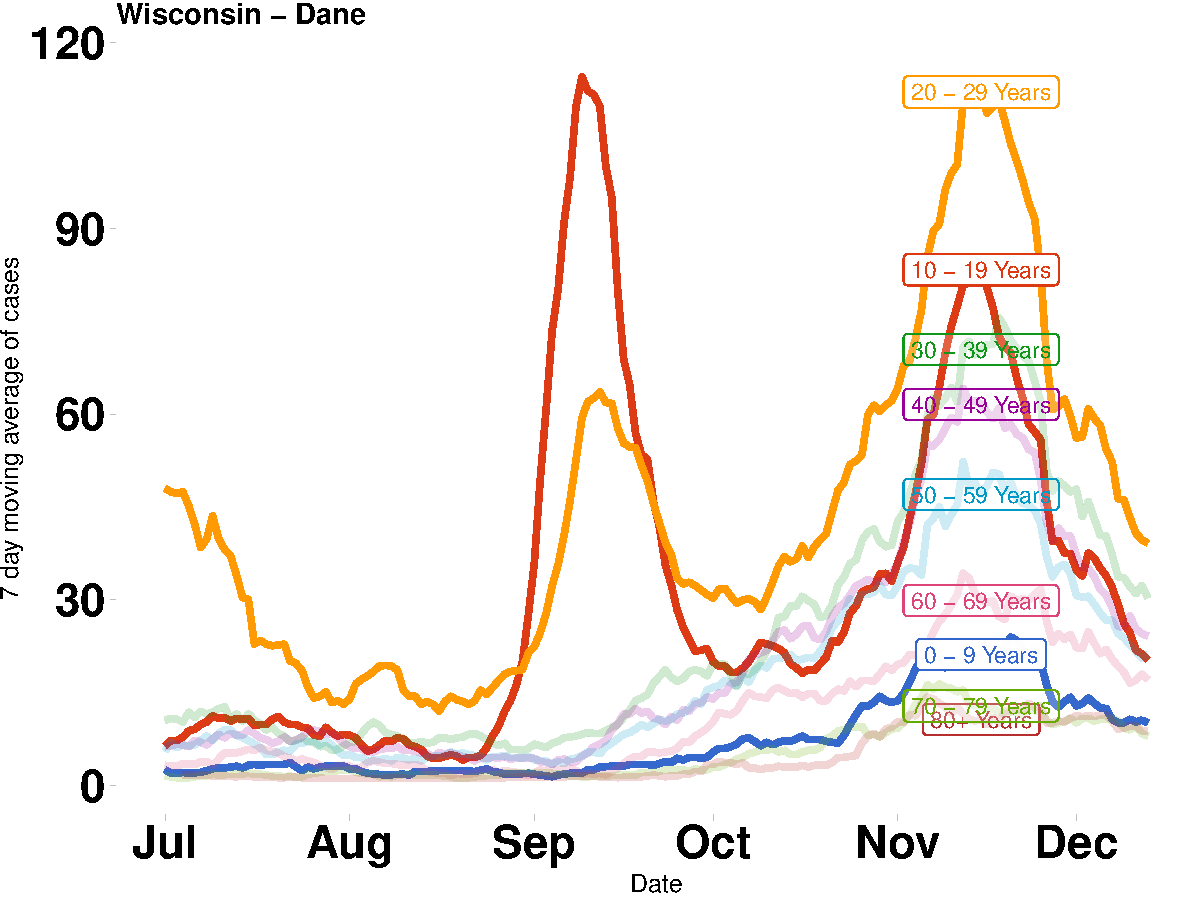
\includegraphics[width=0.50\textwidth]{tables_and_figures/casesByAgeWisconsinDane}&
      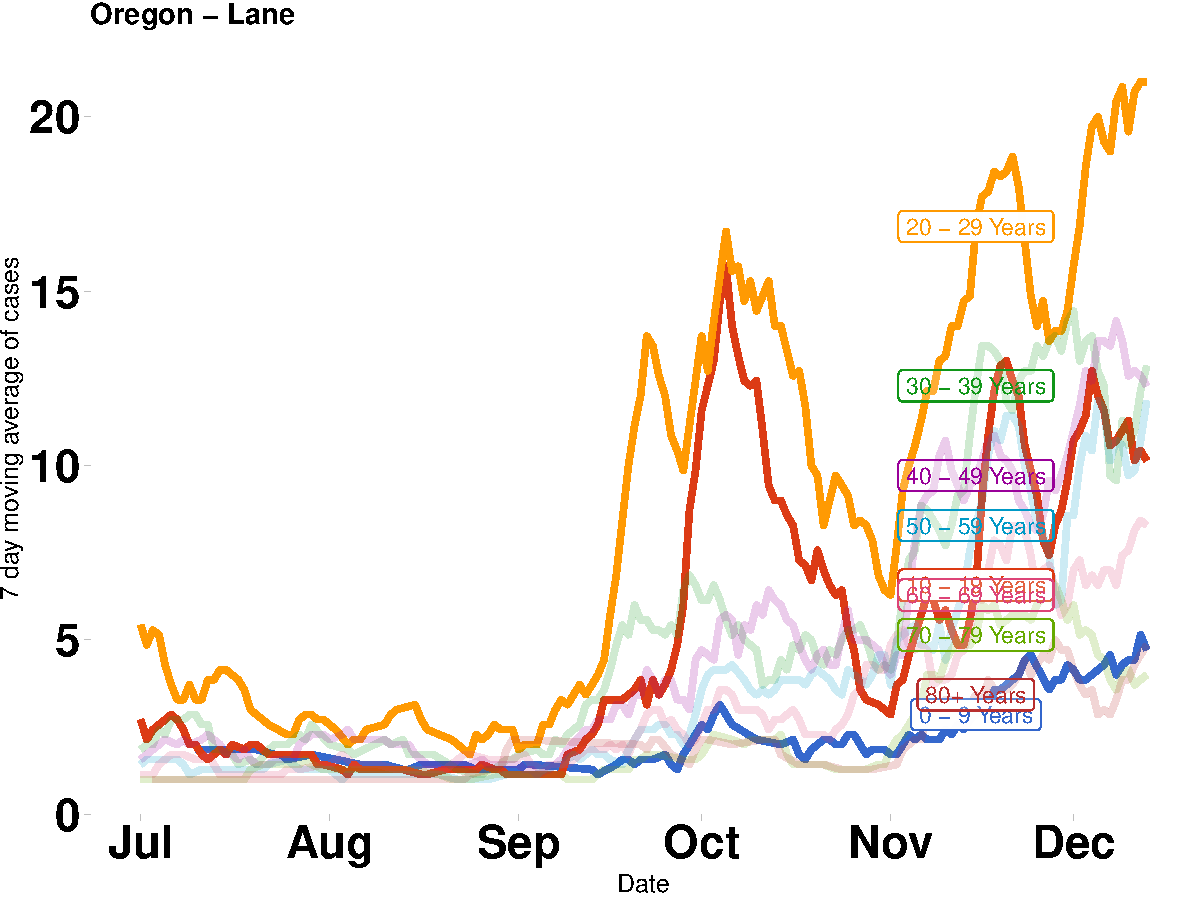
\includegraphics[width=0.50\textwidth]{tables_and_figures/casesByAgeOregonLane}\\
%   School Visits  &  School Visits  \\
%      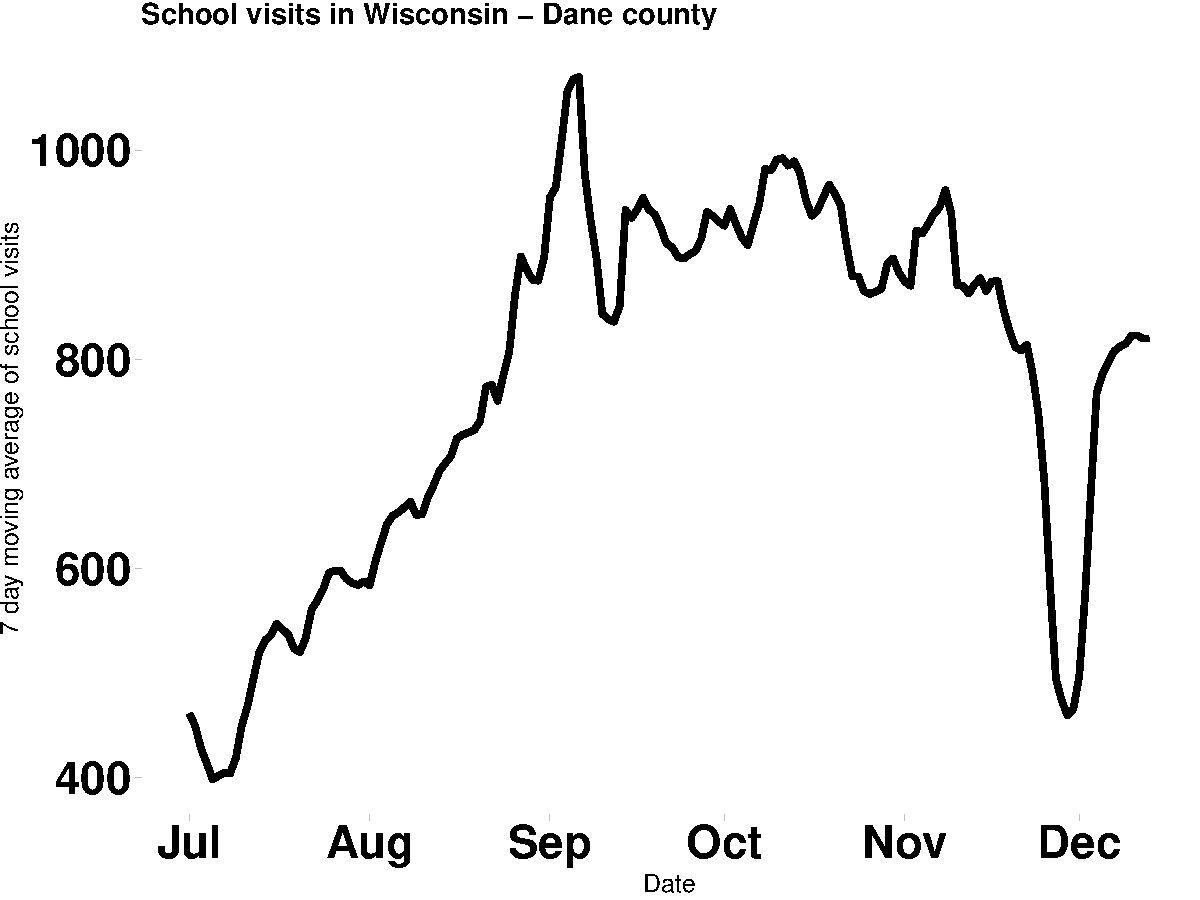
\includegraphics[width=0.50\textwidth,height=0.25\textwidth]{tables_and_figures/schoolWisconsinDane}&
%      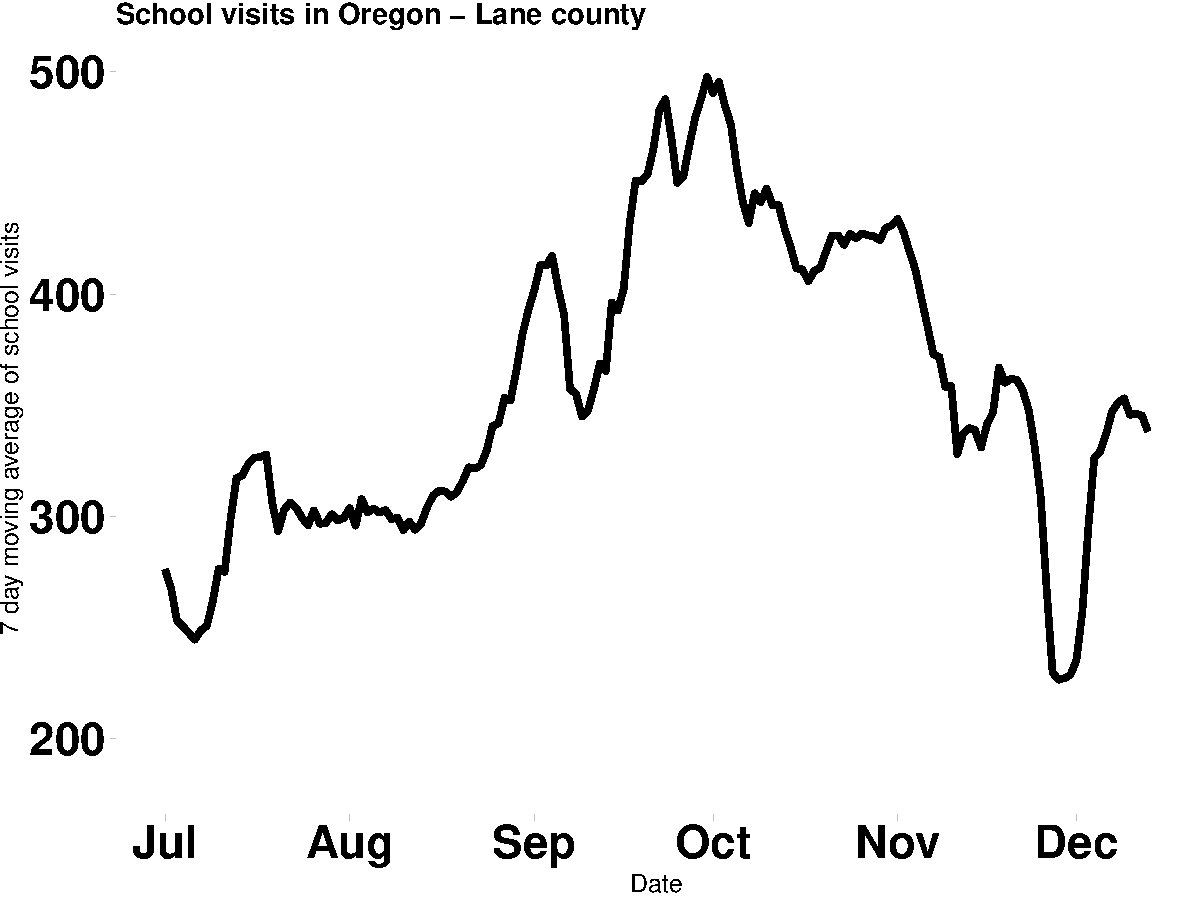
\includegraphics[width=0.50\textwidth,height=0.25\textwidth]{tables_and_figures/schoolOregonLane}\\
    College Visits  &  College Visits  \\
      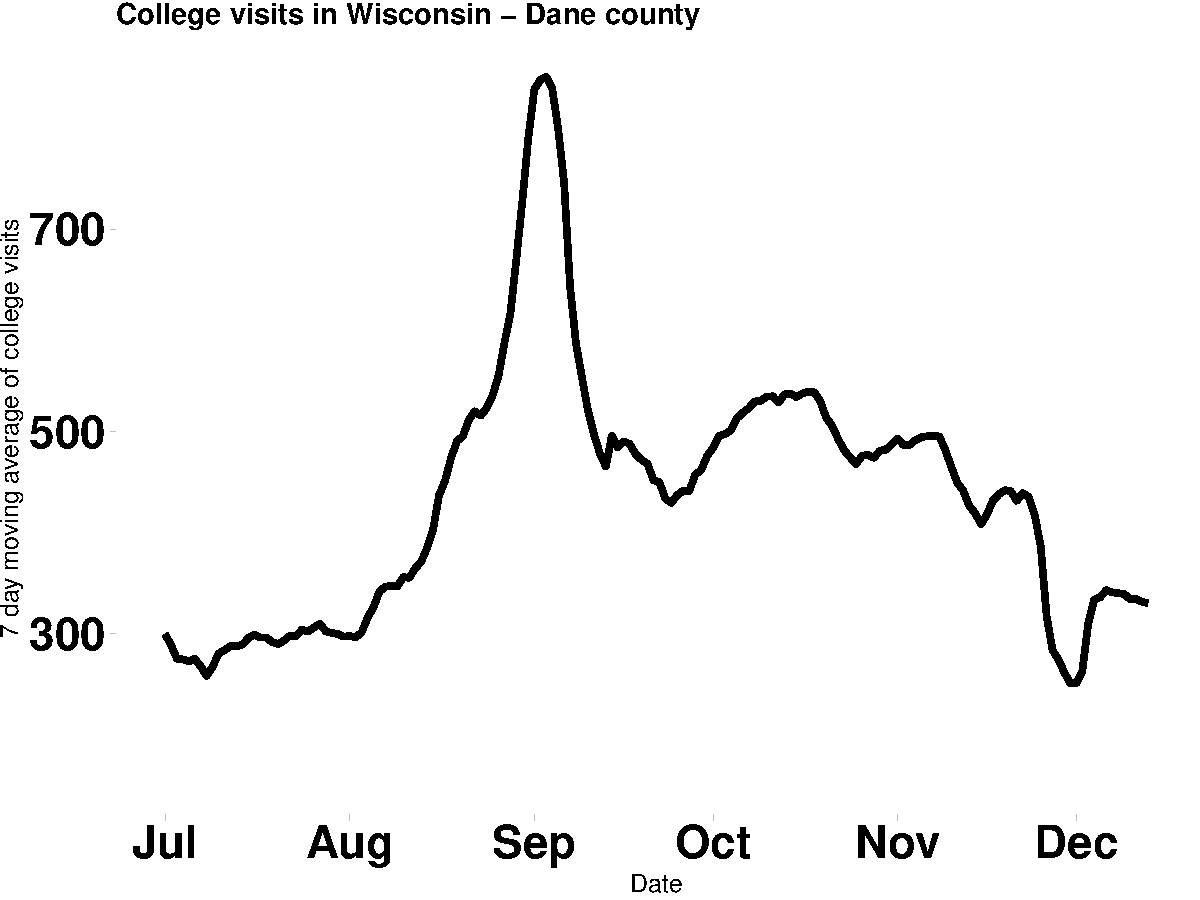
\includegraphics[width=0.50\textwidth,height=0.2\textwidth]{tables_and_figures/collegeWisconsinDane}&
      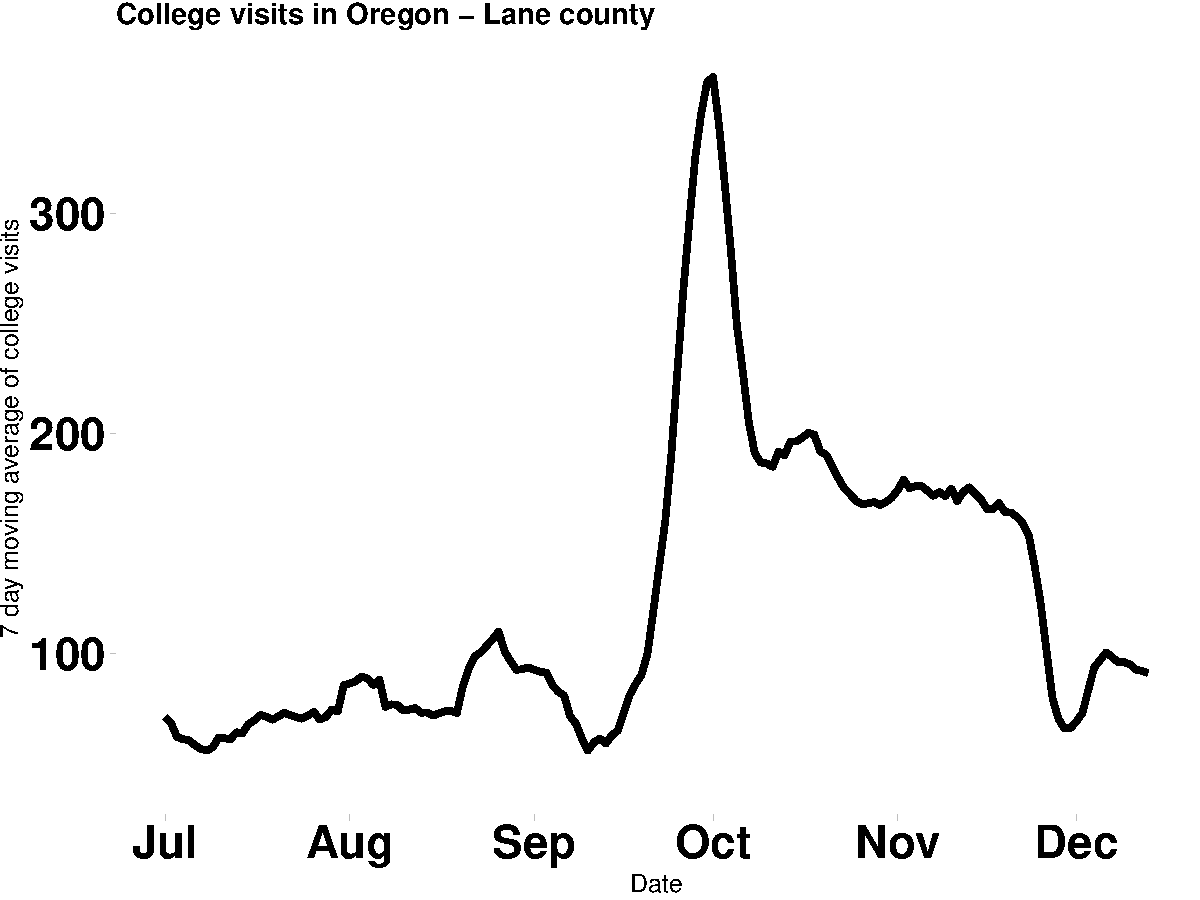
\includegraphics[width=0.50\textwidth,height=0.2\textwidth]{tables_and_figures/collegeOregonLane}\\
  Bar Visits  &  Bar Visits   \\
      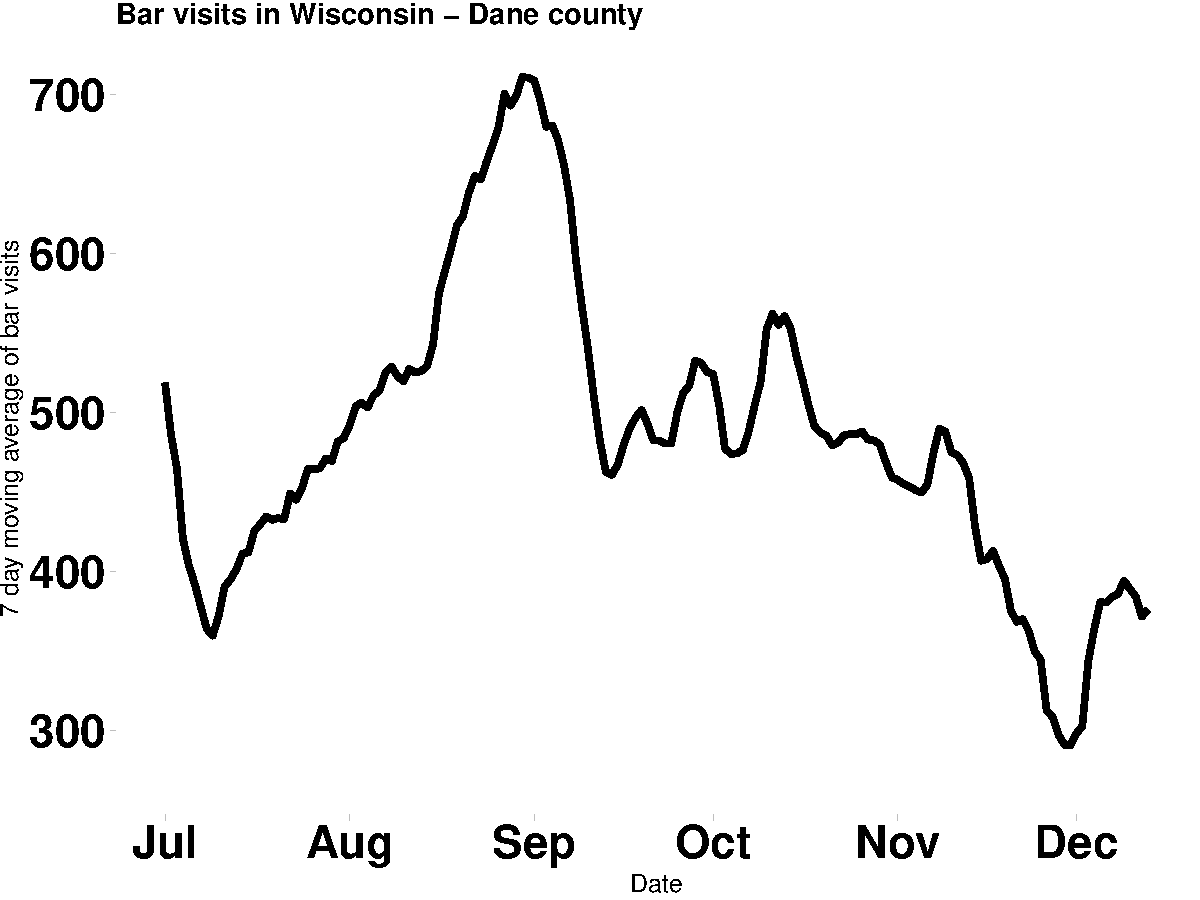
\includegraphics[width=0.50\textwidth,height=0.2\textwidth]{tables_and_figures/barWisconsinDane}&
      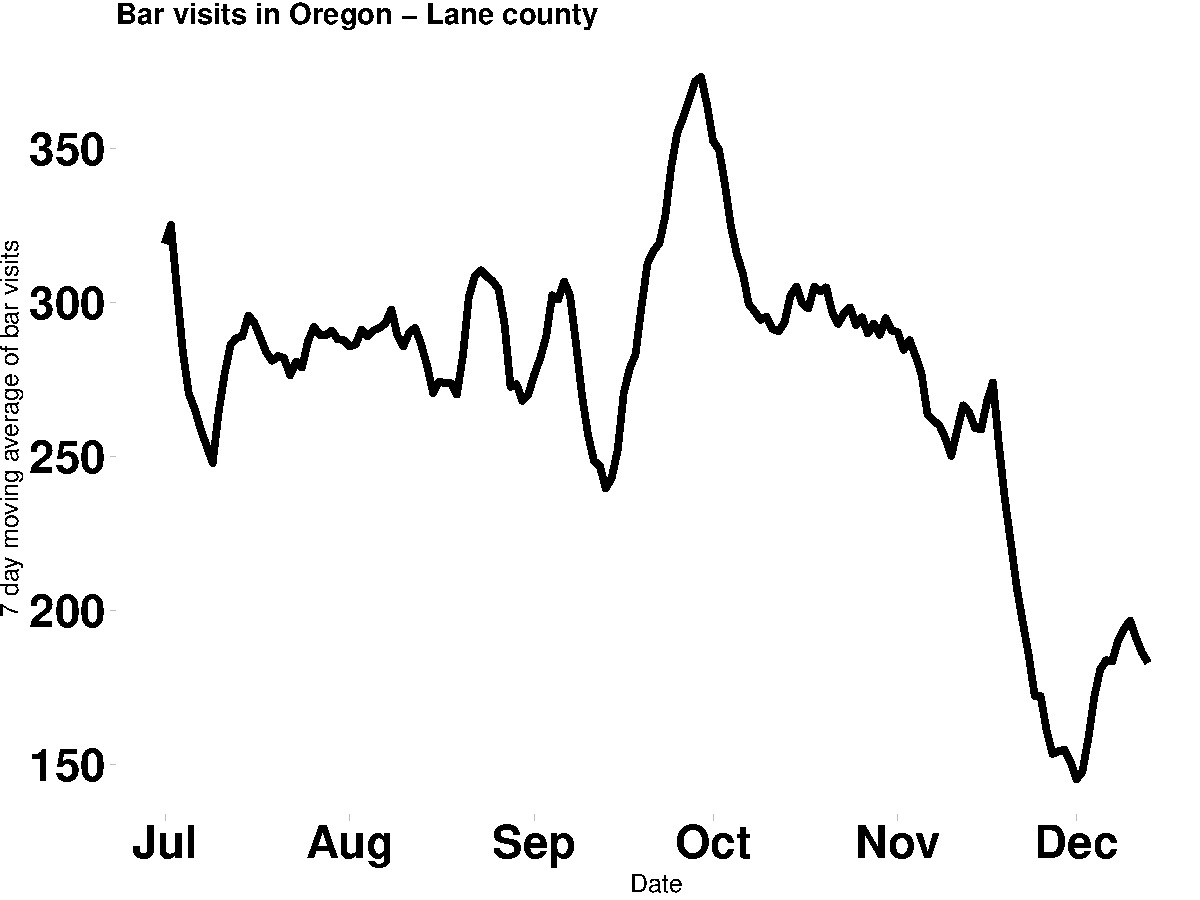
\includegraphics[width=0.50\textwidth,height=0.2\textwidth]{tables_and_figures/barOregonLane}\\
   Restaurant Visits  &  Restaurant Visits   \\
      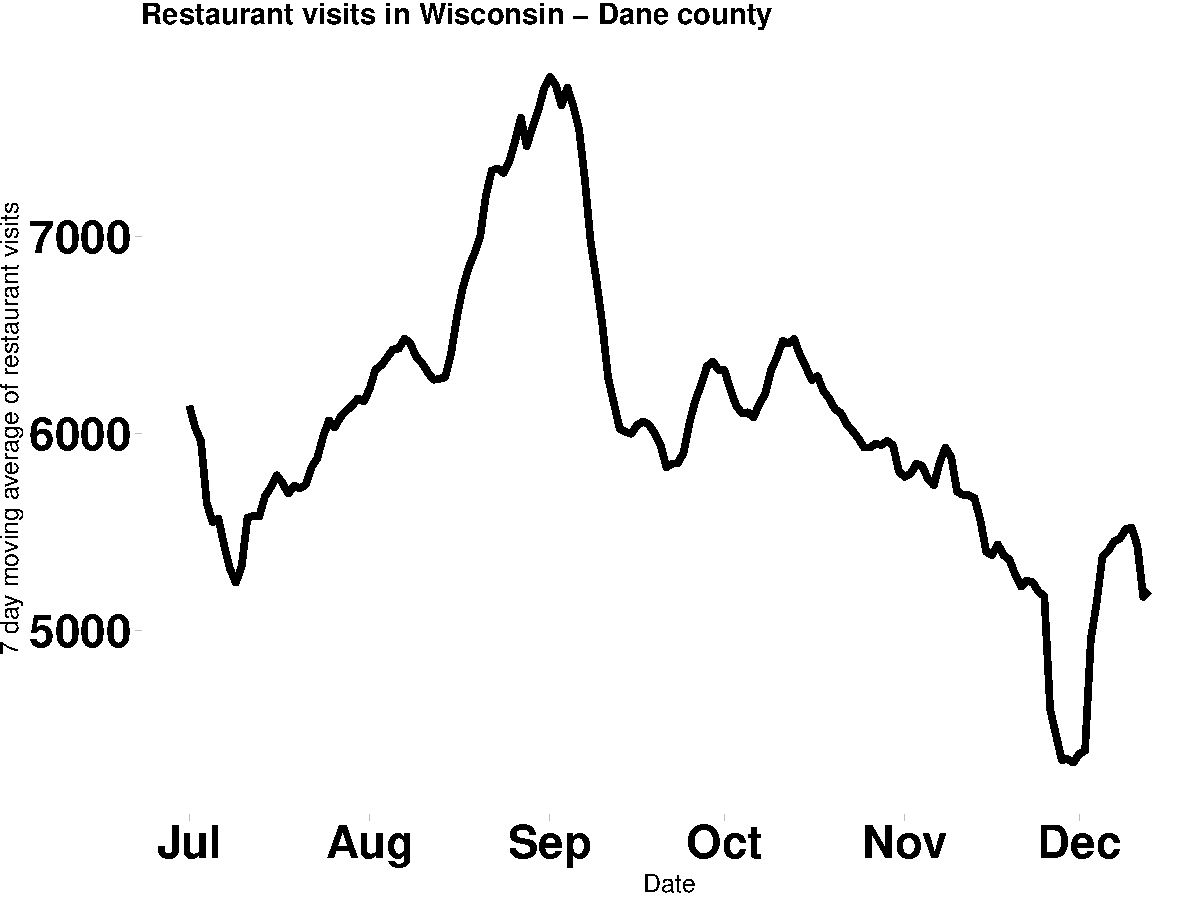
\includegraphics[width=0.50\textwidth,height=0.2\textwidth]{tables_and_figures/restaurantWisconsinDane}&
      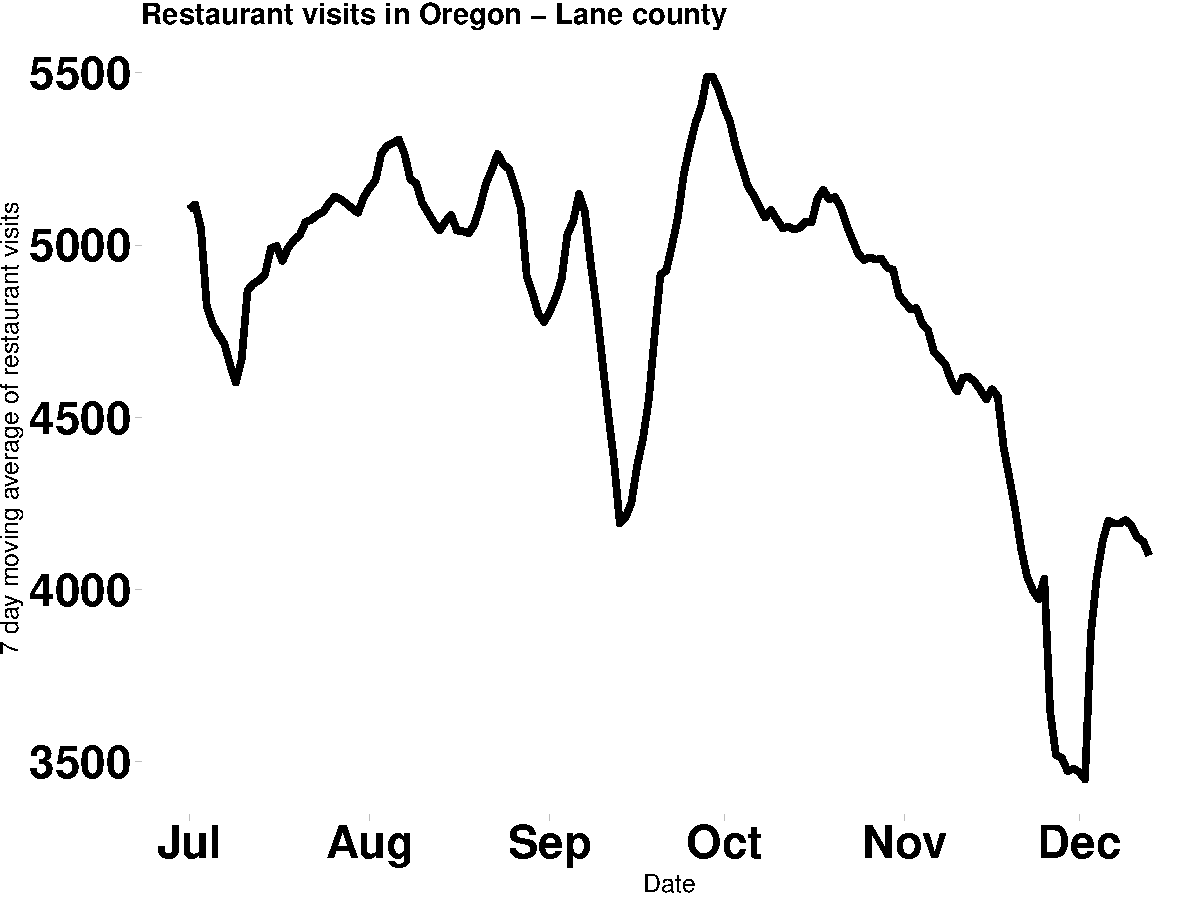
\includegraphics[width=0.50\textwidth,height=0.2\textwidth]{tables_and_figures/restaurantOregonLane}\\
    \end{tabular}
  \end{minipage}}
\vspace{-0.2cm}  {\scriptsize
\begin{flushleft}
Notes:  The first, the second, and the third figures in the left panel show the evolution of the number of cases by age groups, the number of visits to colleges/universities, and bars, respectively, in Dane County, WI. The right panel shows the corresponding figures for Lane County, OR.
 \end{flushleft}    }
 \end{figure}

   
\begin{figure}[!ht] 
  \caption{The number of cases by age groups and the number of visits to colleges/universities,  bars, restaurants, recreation facilities,   K-12 schools,  and a comparison of reported cases between CDC and NYT data \label{fig:dane-SI}} 
  \resizebox{0.9\columnwidth}{!}{
\begin{minipage}{\linewidth} 
        \begin{tabular}{c|c|c|c|c}  
         \large{ \textbf{ Pima, AZ} }&   \large {  \textbf{Ingham, MI}}&  \large  {  \textbf{Centre, PA }}& 
          \large  { \textbf{Story, IA}}&   \large {  \textbf{Champaign, IL}}\\ \hline
   Cases by Age Groups &  Cases by Age Groups &  Cases by Age Groups &  Cases by Age Groups& Cases by Age Groups  \\ 
      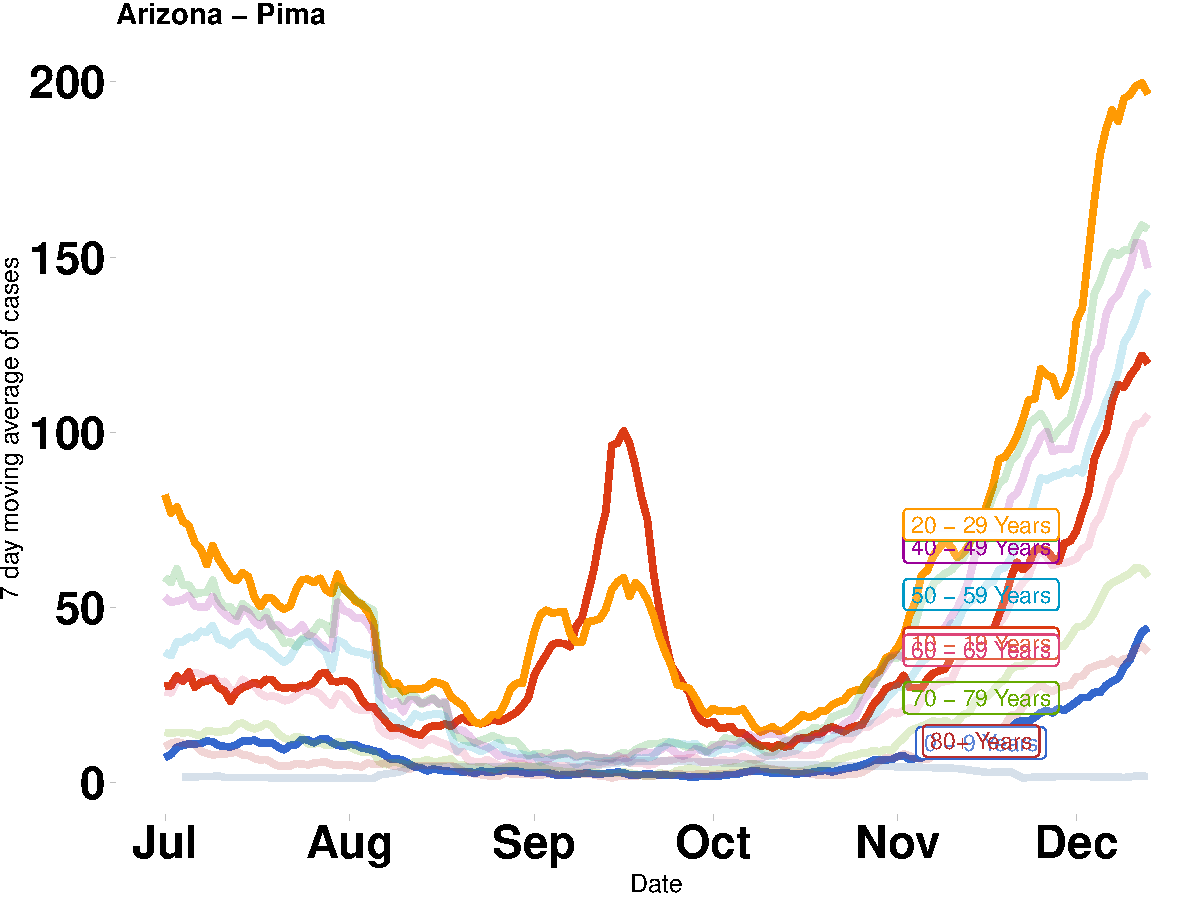
\includegraphics[width=0.20\textwidth]{tables_and_figures/casesByAgeArizonaPima}&
      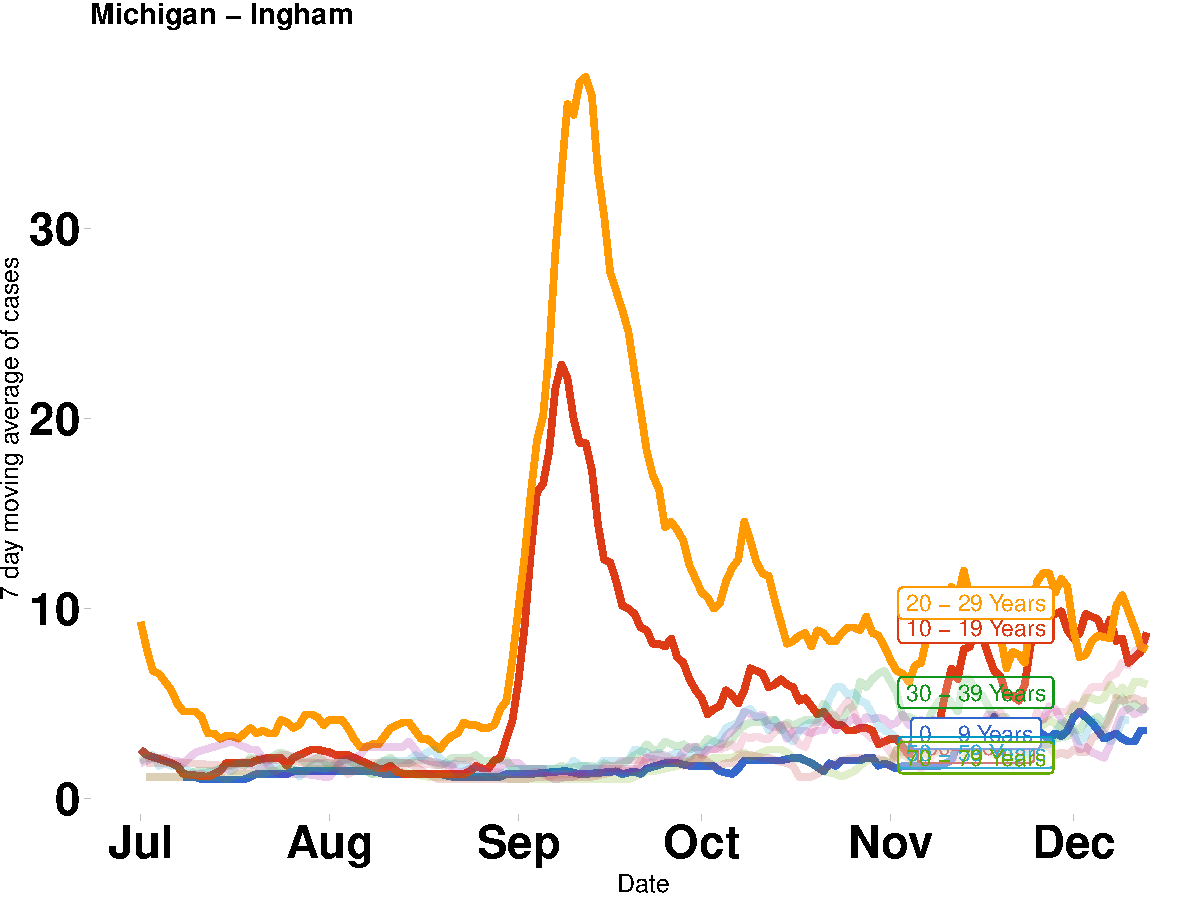
\includegraphics[width=0.20\textwidth]{tables_and_figures/casesByAgeMichiganIngham}&
      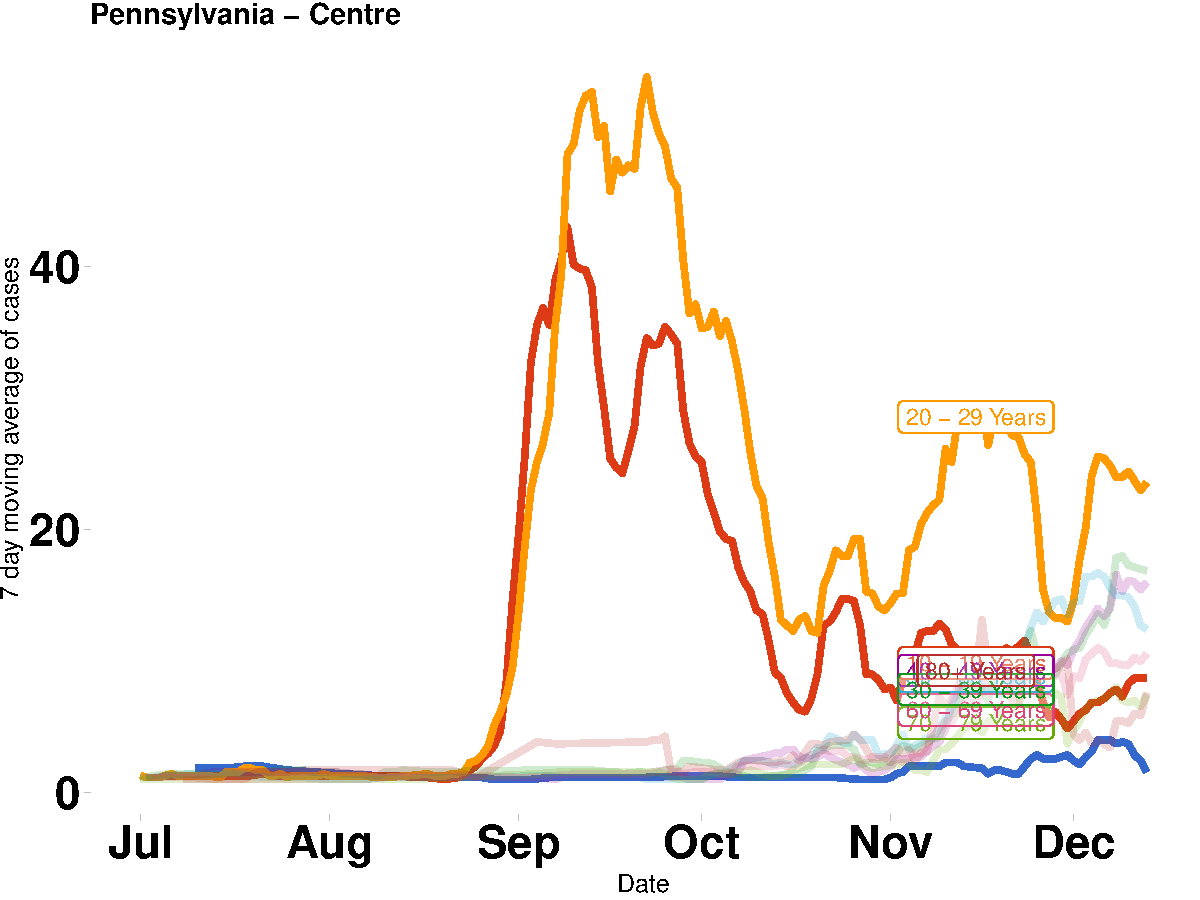
\includegraphics[width=0.20\textwidth]{tables_and_figures/casesByAgePennsylvaniaCentre}&
      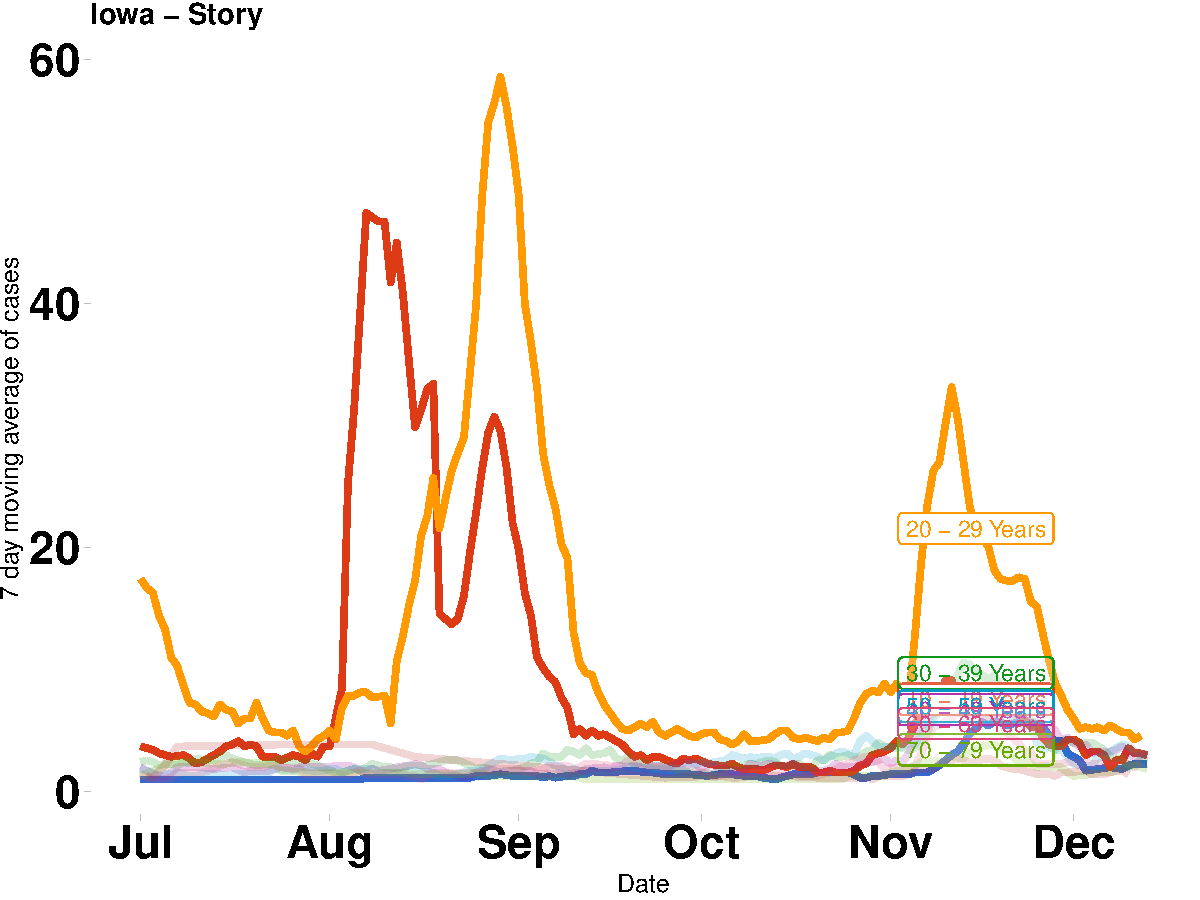
\includegraphics[width=0.20\textwidth]{tables_and_figures/casesByAgeIowaStory}& 
      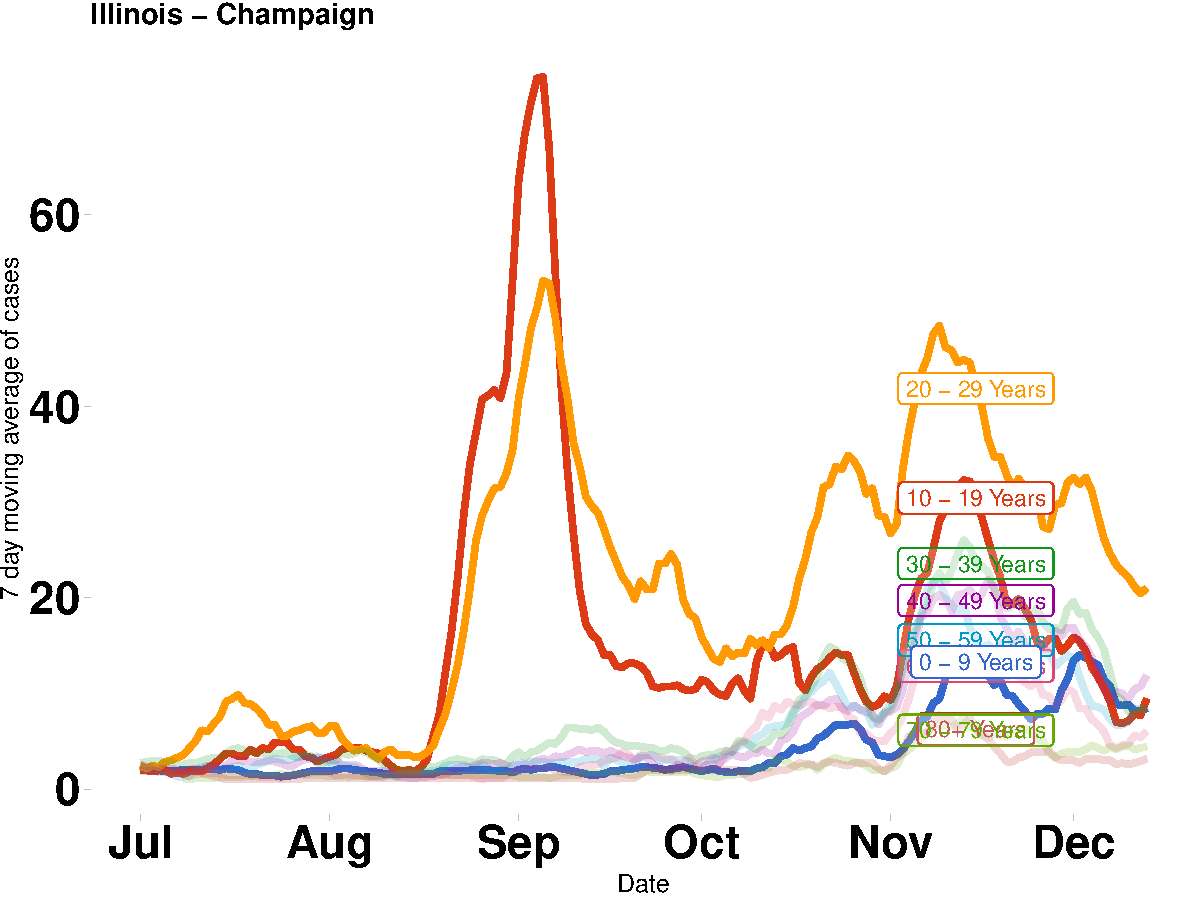
\includegraphics[width=0.20\textwidth]{tables_and_figures/casesByAgeIllinoisChampaign}\\  
   College Visits  &  College Visits  & College Visits  &  College Visits  & College Visits  \\   
      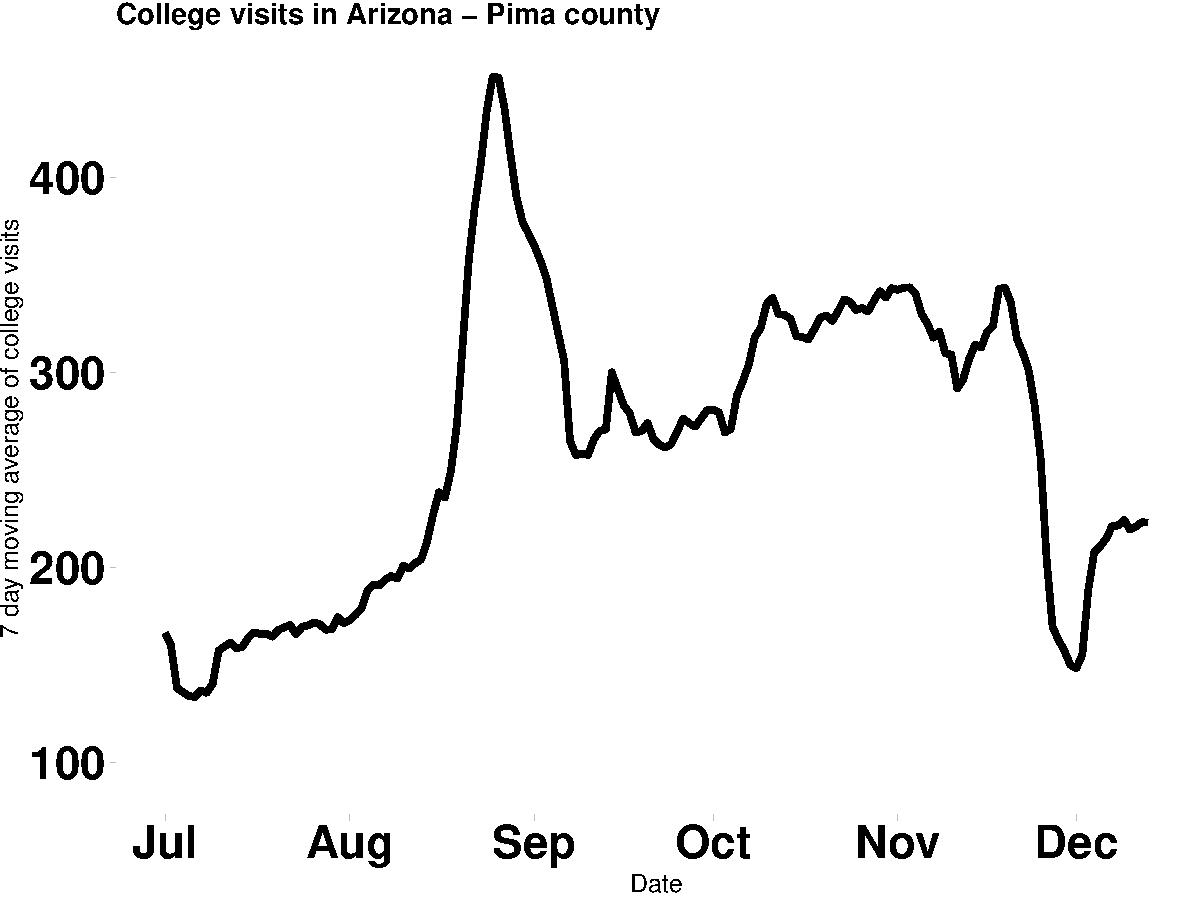
\includegraphics[width=0.20\textwidth]{tables_and_figures/collegeArizonaPima}&
      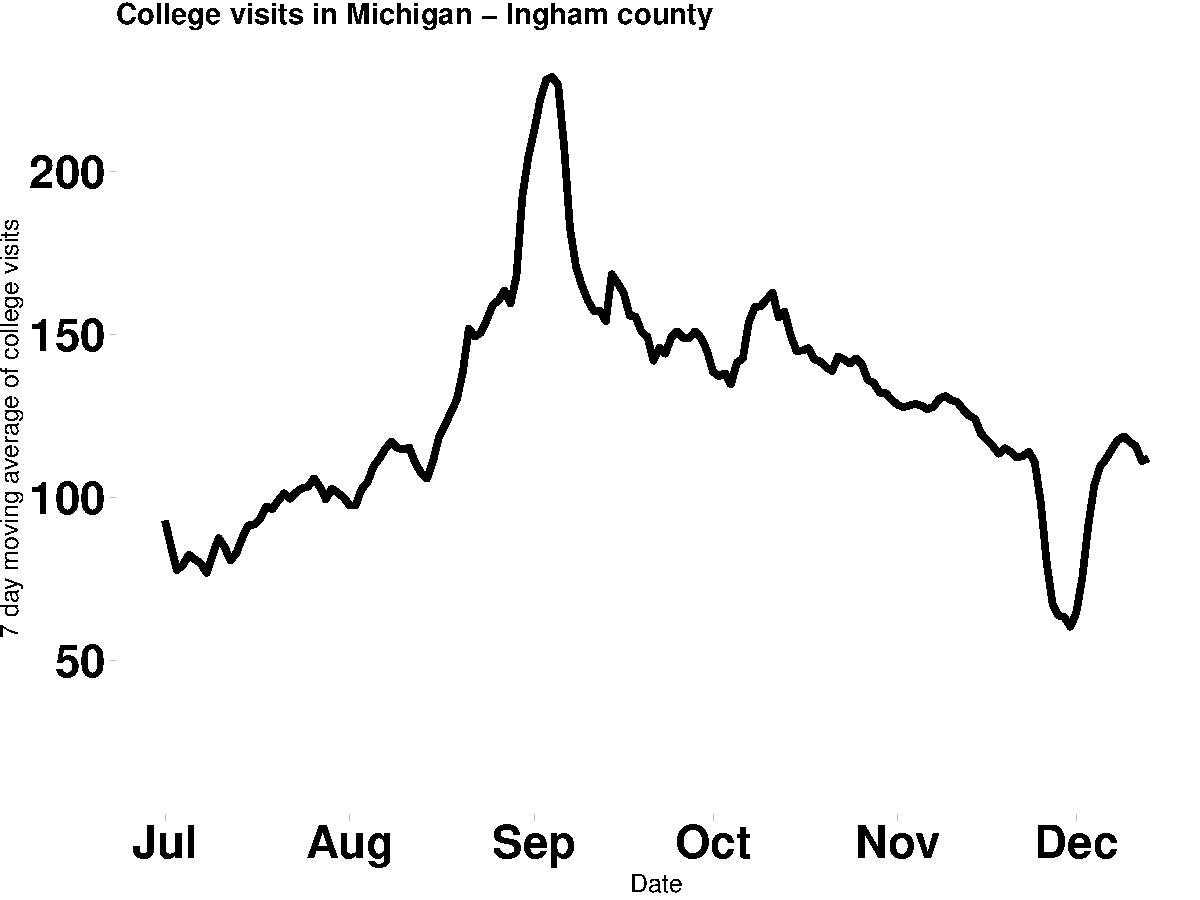
\includegraphics[width=0.20\textwidth]{tables_and_figures/collegeMichiganIngham}&
      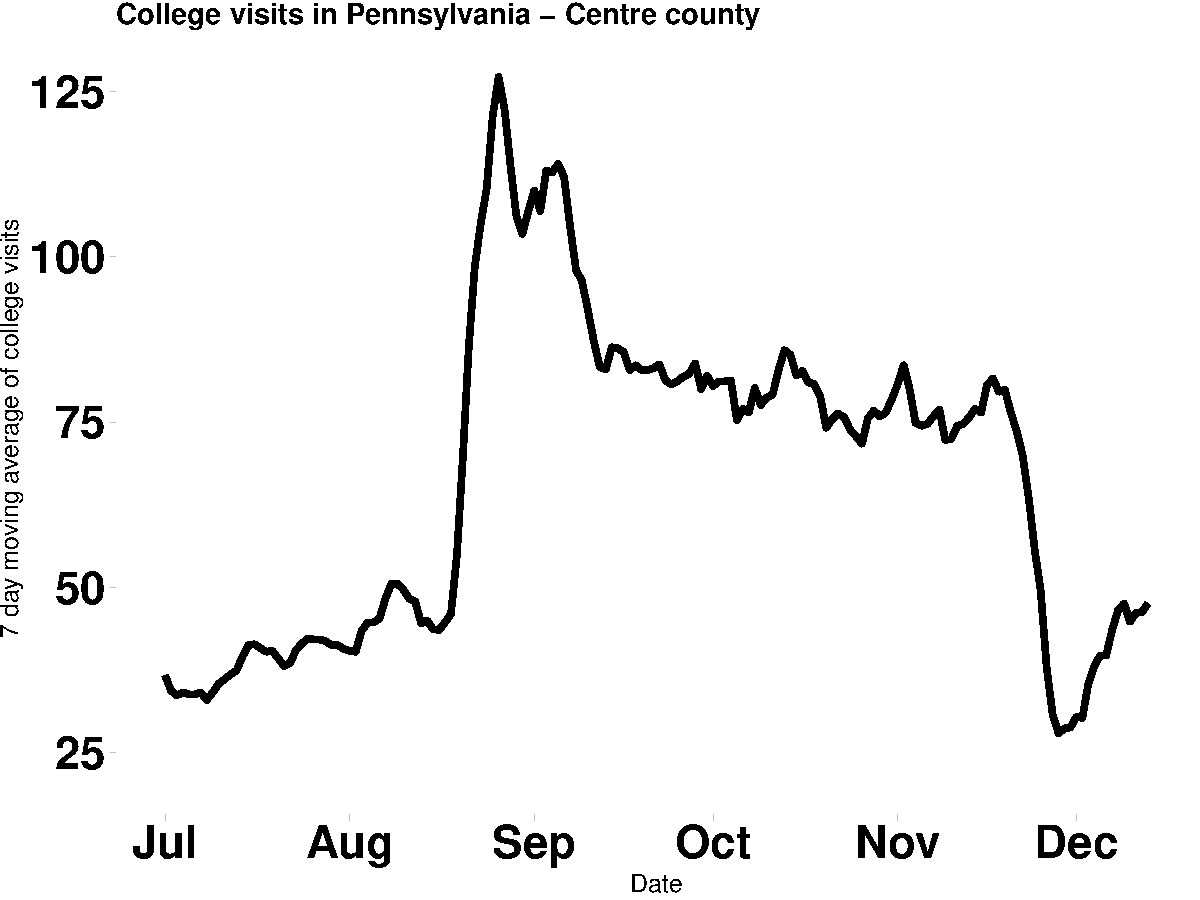
\includegraphics[width=0.20\textwidth]{tables_and_figures/collegePennsylvaniaCentre}&
      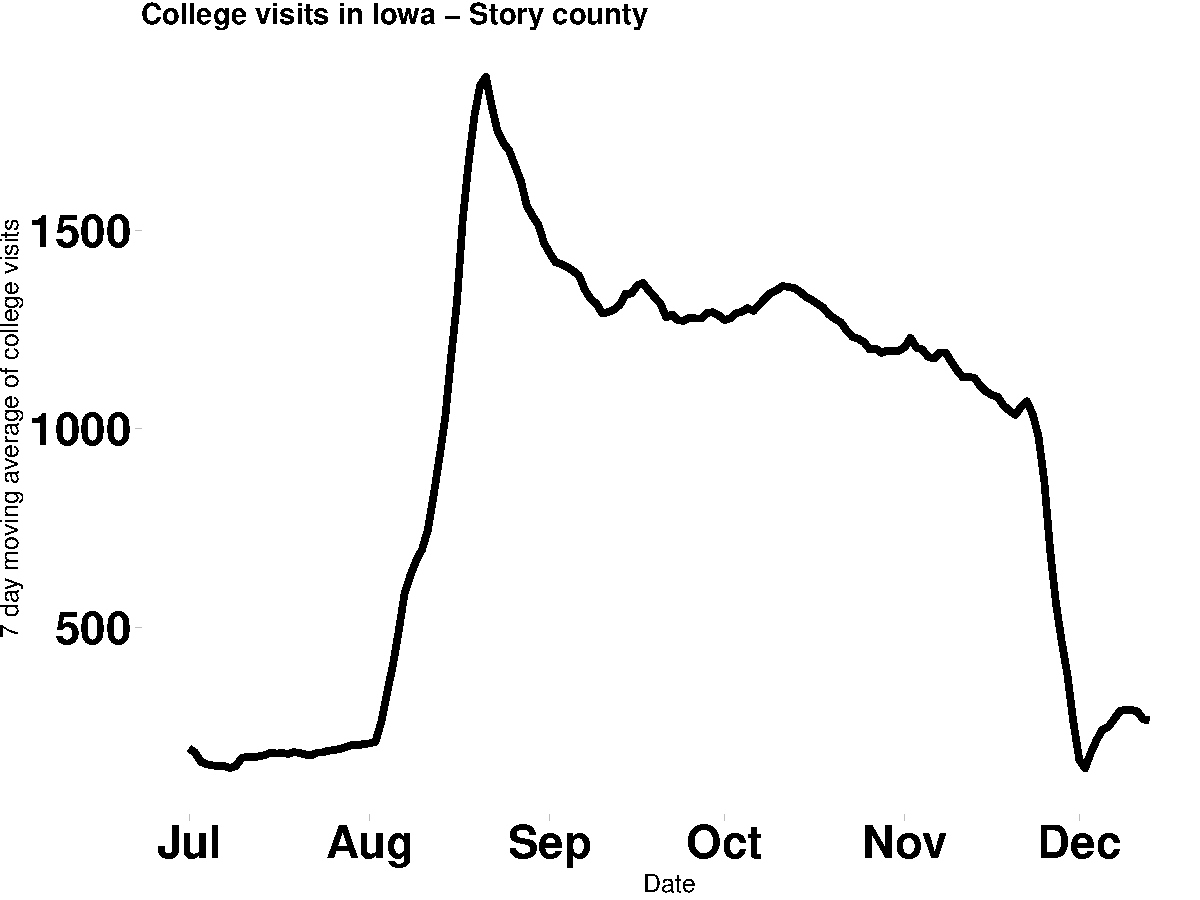
\includegraphics[width=0.20\textwidth]{tables_and_figures/collegeIowaStory}& 
      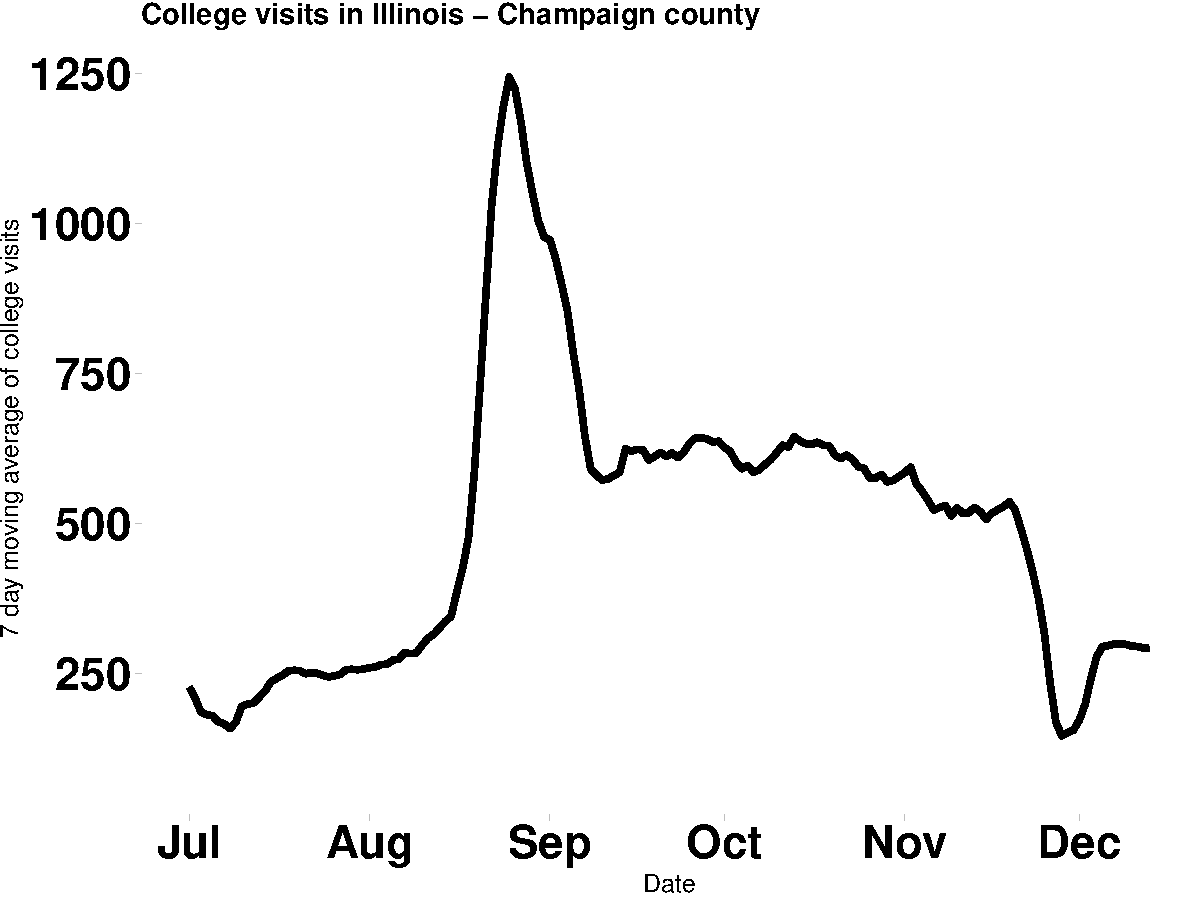
\includegraphics[width=0.20\textwidth]{tables_and_figures/collegeIllinoisChampaign}\\  
   Bar Visits  &  Bar Visits & Bar Visits  &  Bar Visits & Bar Visits     \\  
      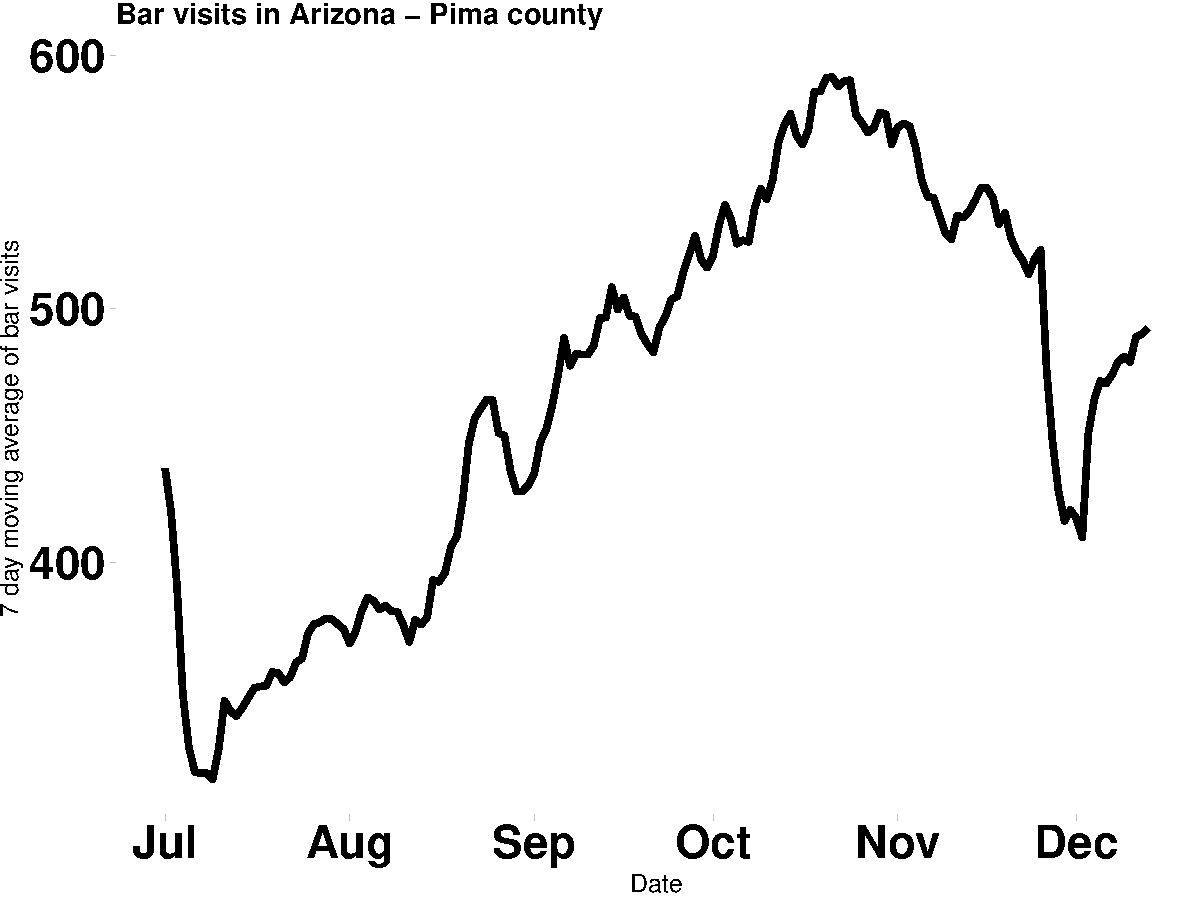
\includegraphics[width=0.20\textwidth]{tables_and_figures/barArizonaPima}&
      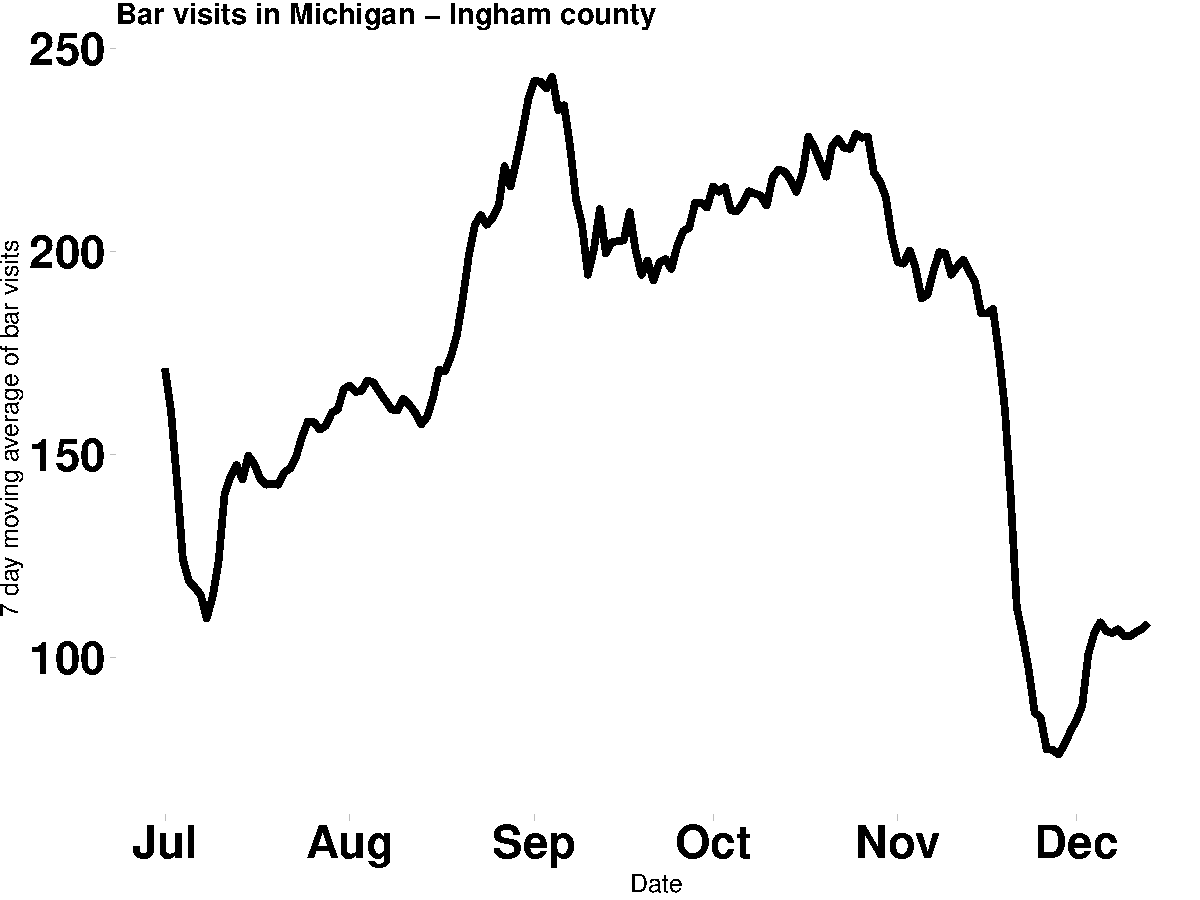
\includegraphics[width=0.20\textwidth]{tables_and_figures/barMichiganIngham}&
      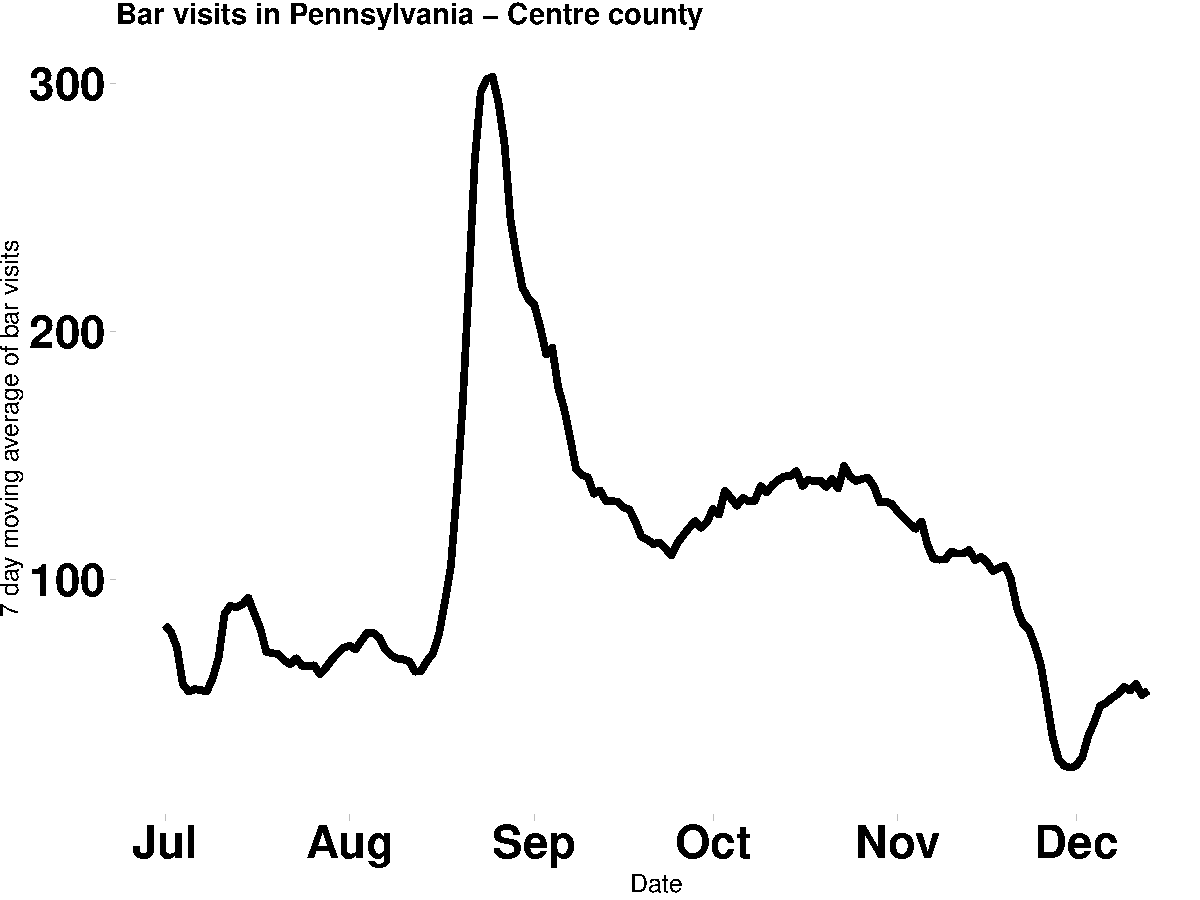
\includegraphics[width=0.20\textwidth]{tables_and_figures/barPennsylvaniaCentre}&
      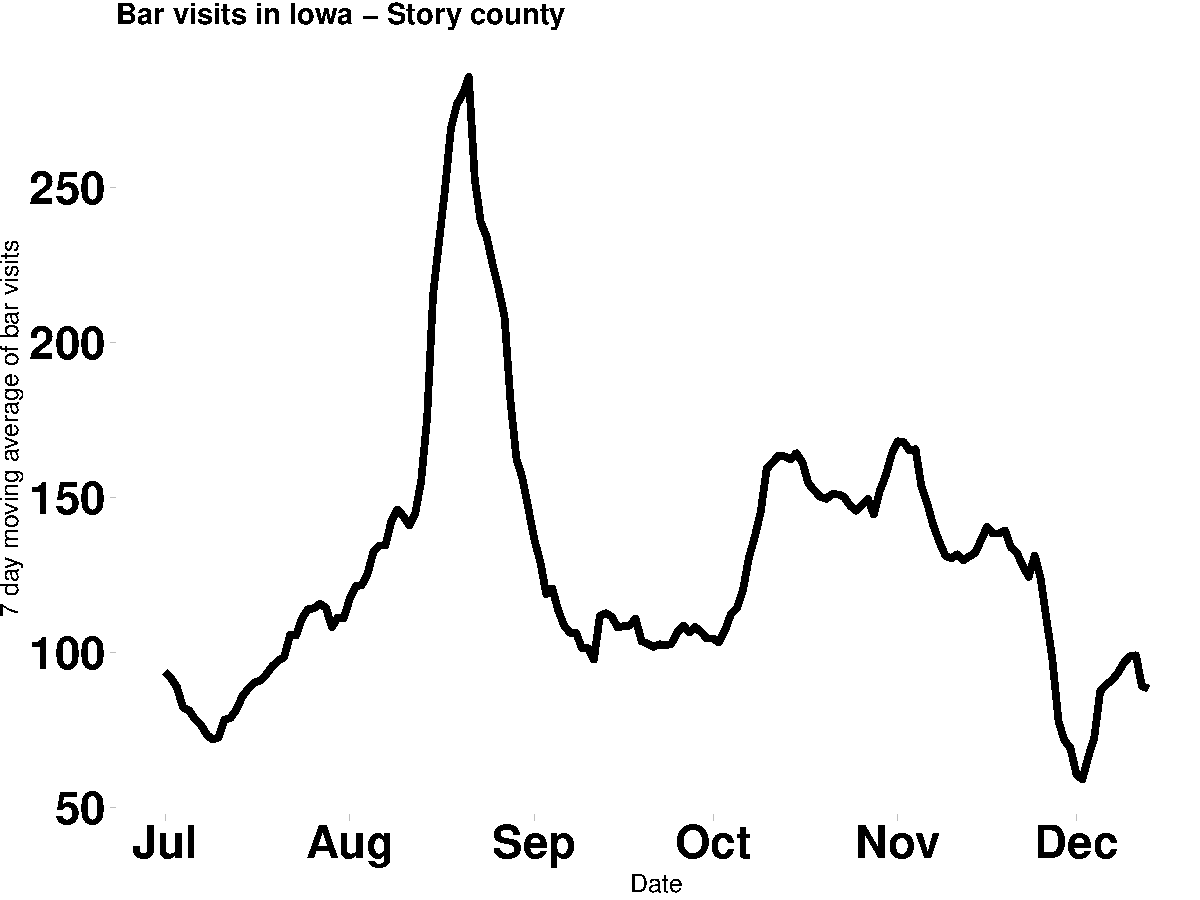
\includegraphics[width=0.20\textwidth]{tables_and_figures/barIowaStory}& 
      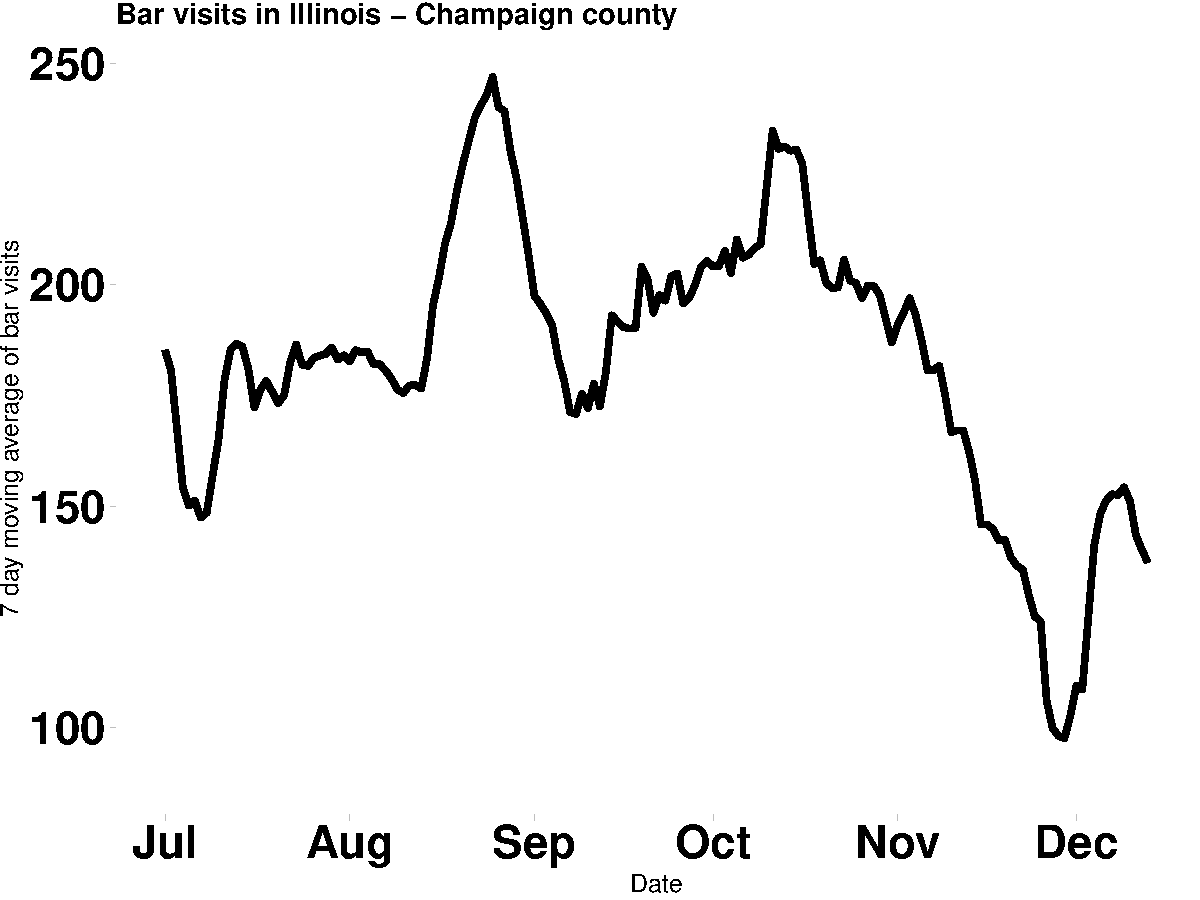
\includegraphics[width=0.20\textwidth]{tables_and_figures/barIllinoisChampaign}\\     
   Restaurant Visits  &  Restaurant Visits  & Restaurant Visits  &  Restaurant Visits  & Restaurant Visits    \\ 
      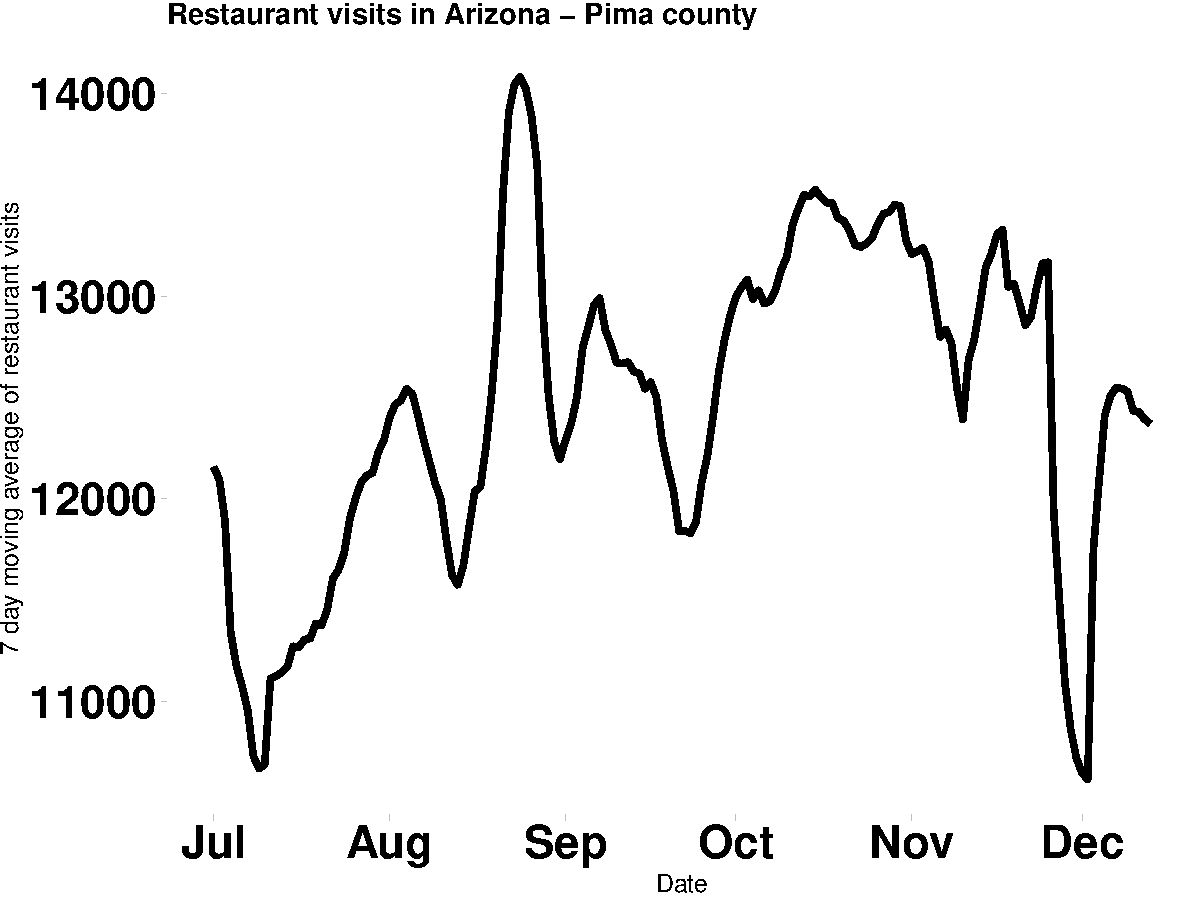
\includegraphics[width=0.20\textwidth]{tables_and_figures/restaurantArizonaPima}&
      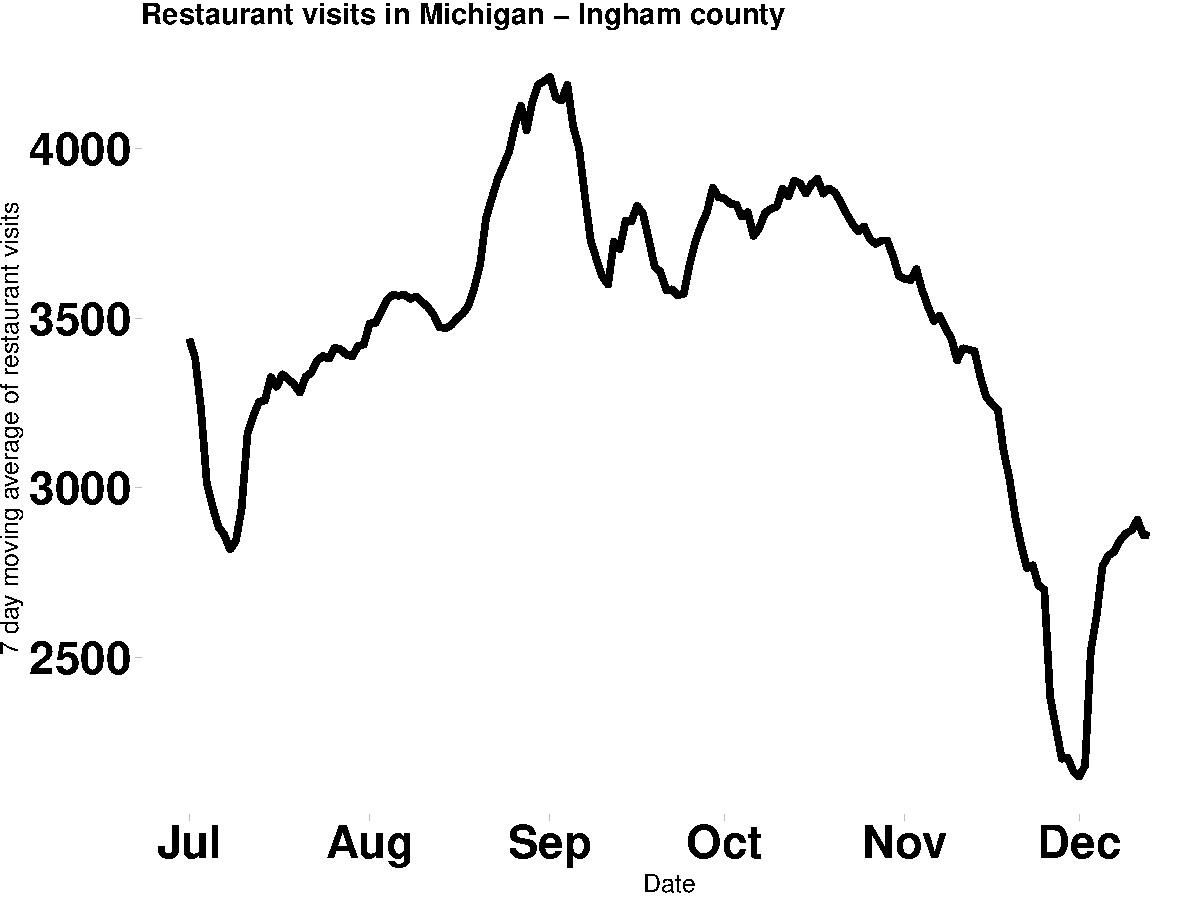
\includegraphics[width=0.20\textwidth]{tables_and_figures/restaurantMichiganIngham}&
      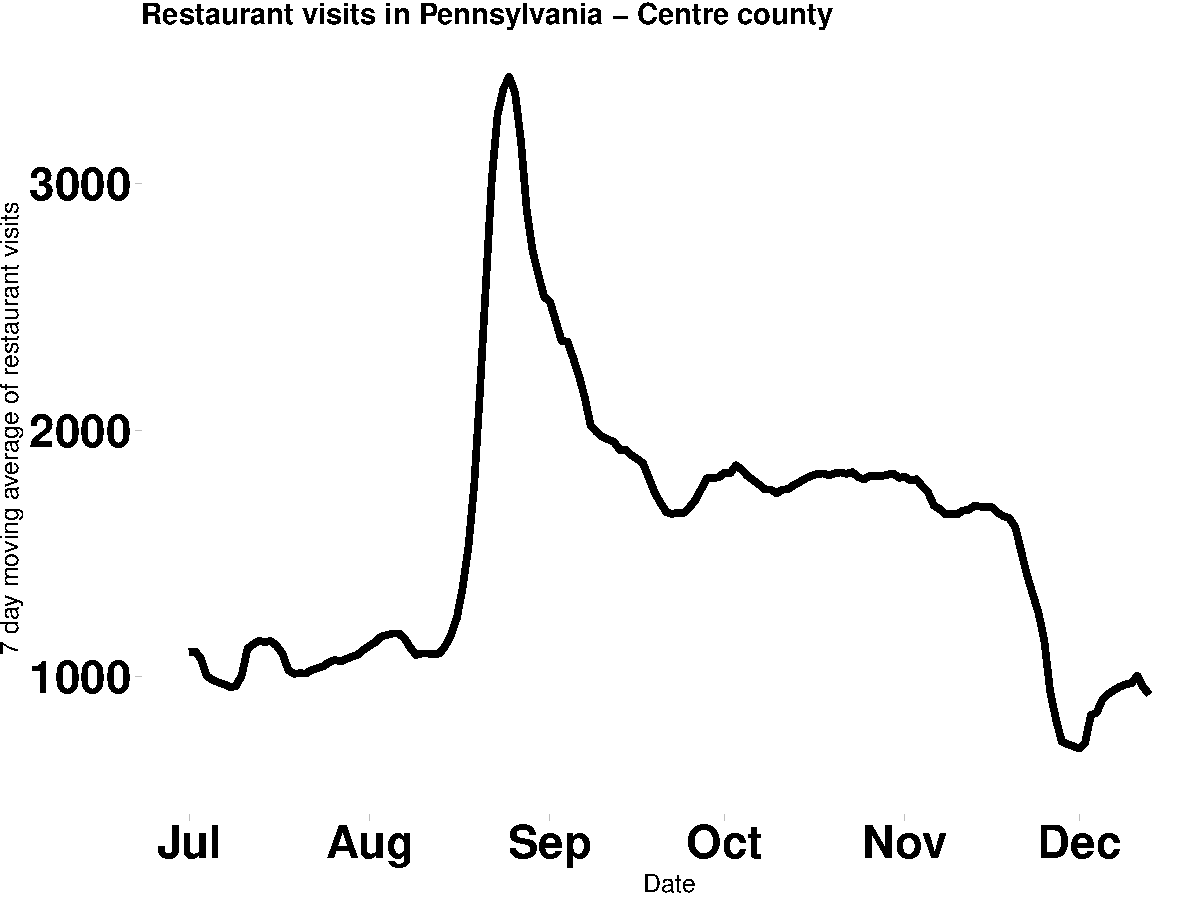
\includegraphics[width=0.20\textwidth]{tables_and_figures/restaurantPennsylvaniaCentre}&
      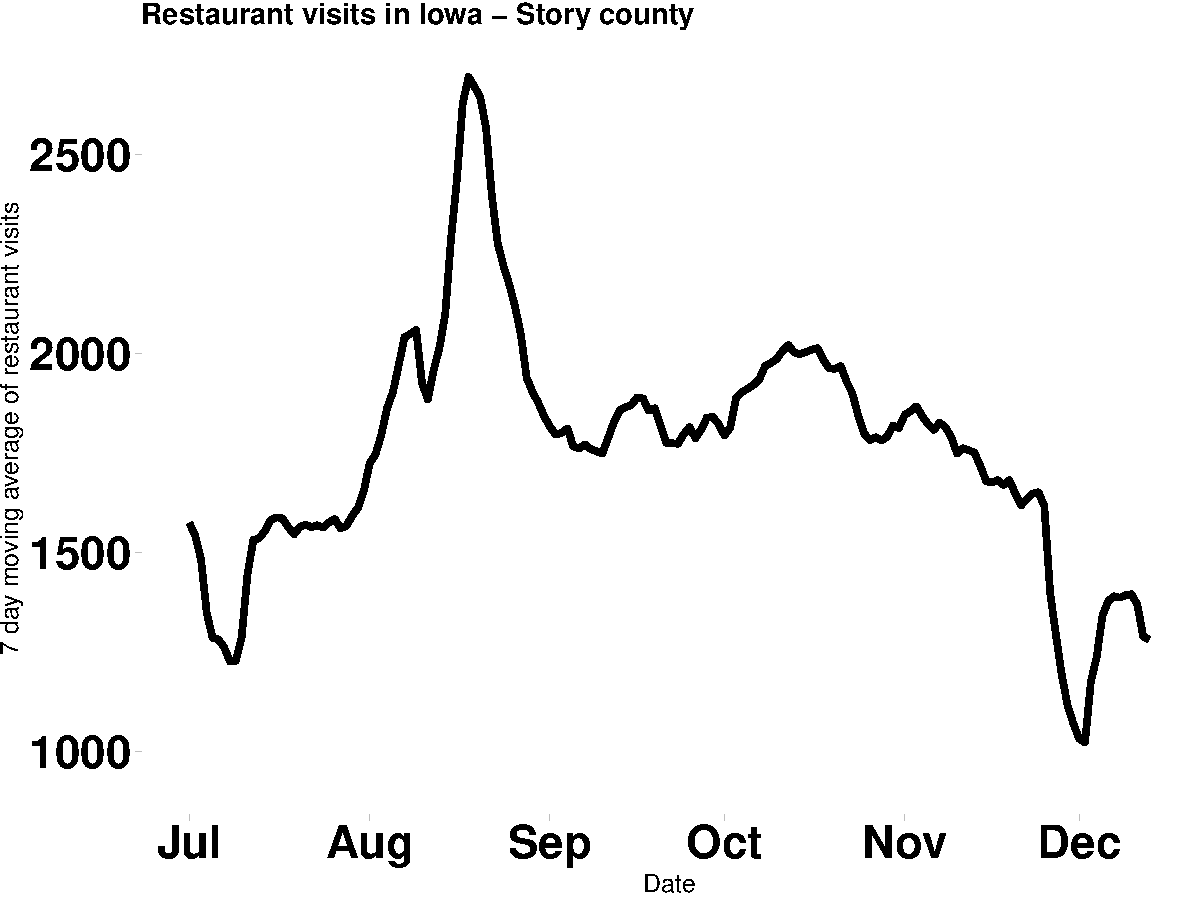
\includegraphics[width=0.20\textwidth]{tables_and_figures/restaurantIowaStory}& 
      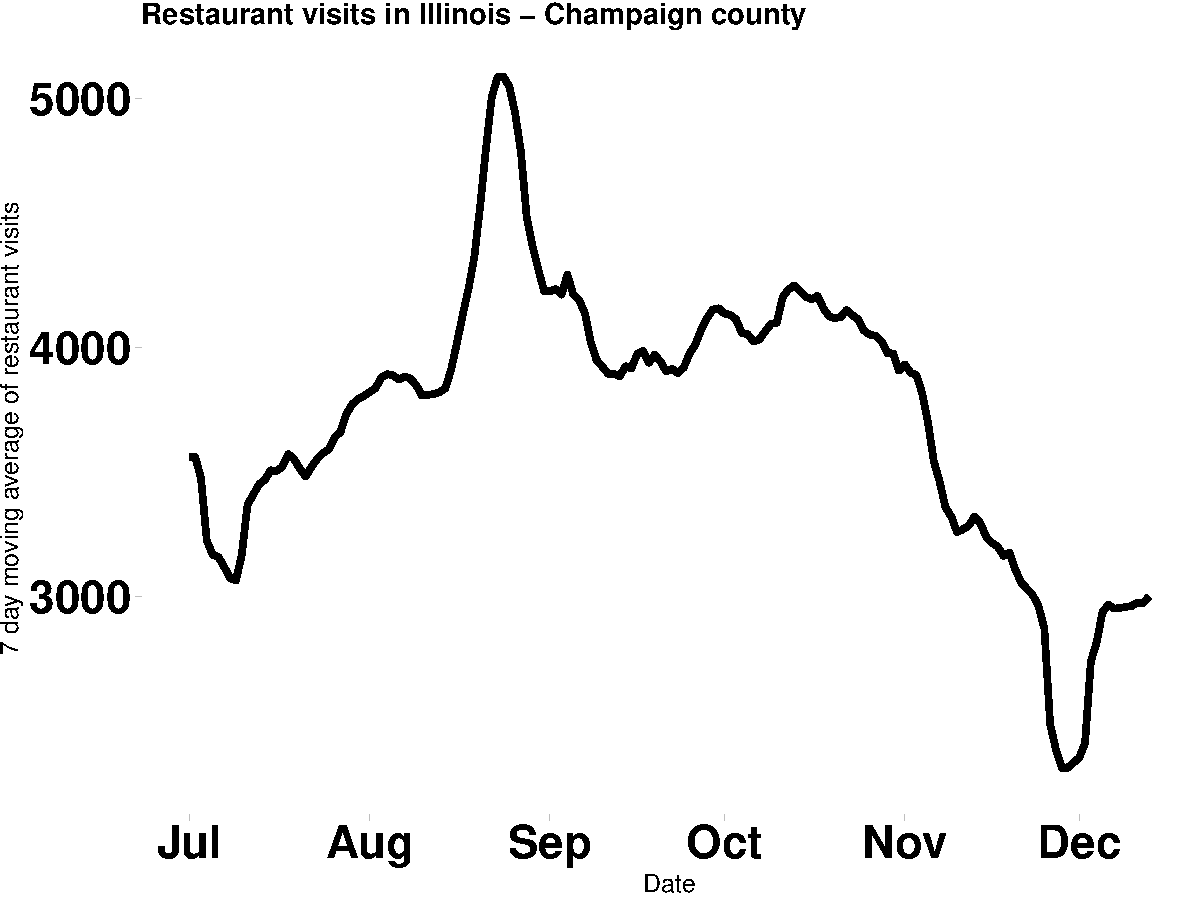
\includegraphics[width=0.20\textwidth]{tables_and_figures/restaurantIllinoisChampaign}\\   
   Recreation Facilitiy Visits  &  Recreation Facilitiy Visits  & Recreation Facilitiy Visits  &  Recreation Facilitiy Visits& Recreation Facilitiy Visits     \\  
      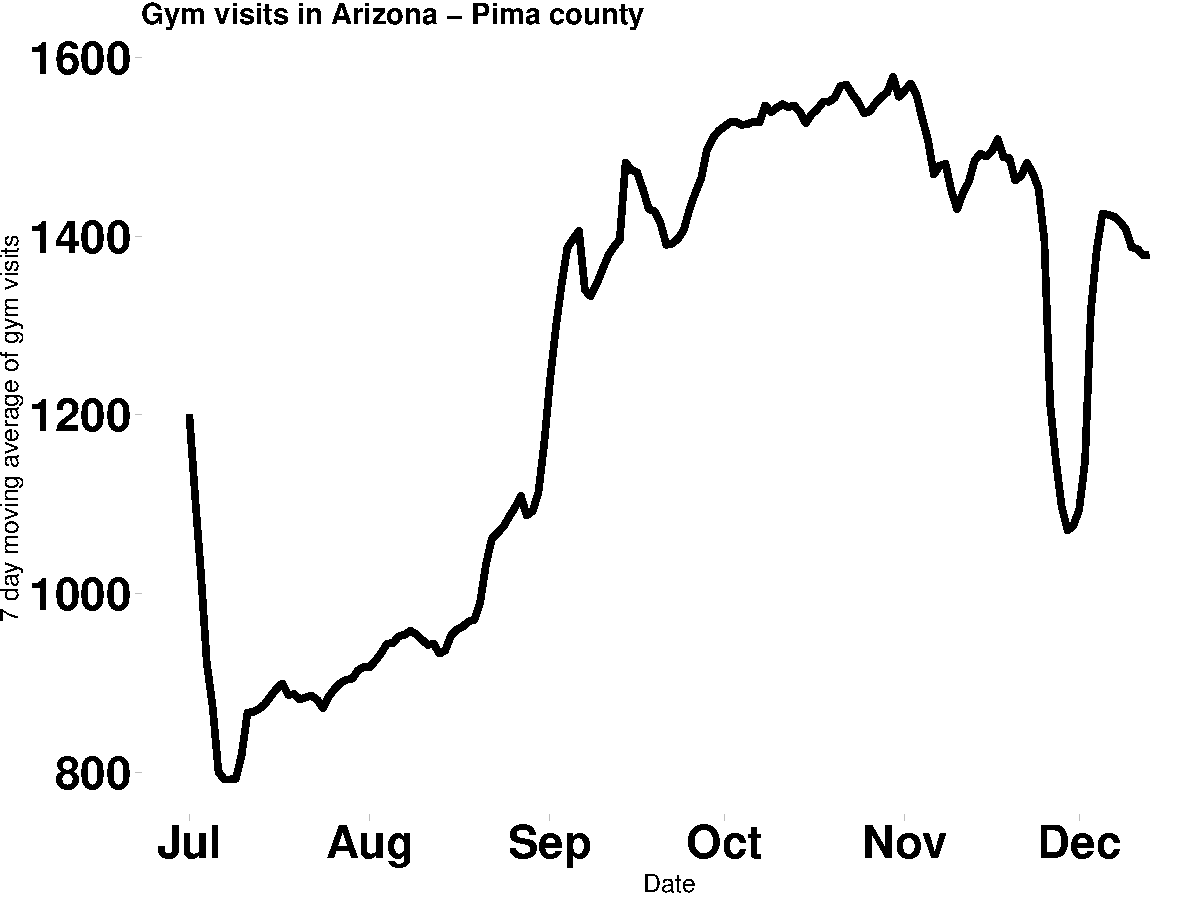
\includegraphics[width=0.20\textwidth]{tables_and_figures/gymArizonaPima}&
      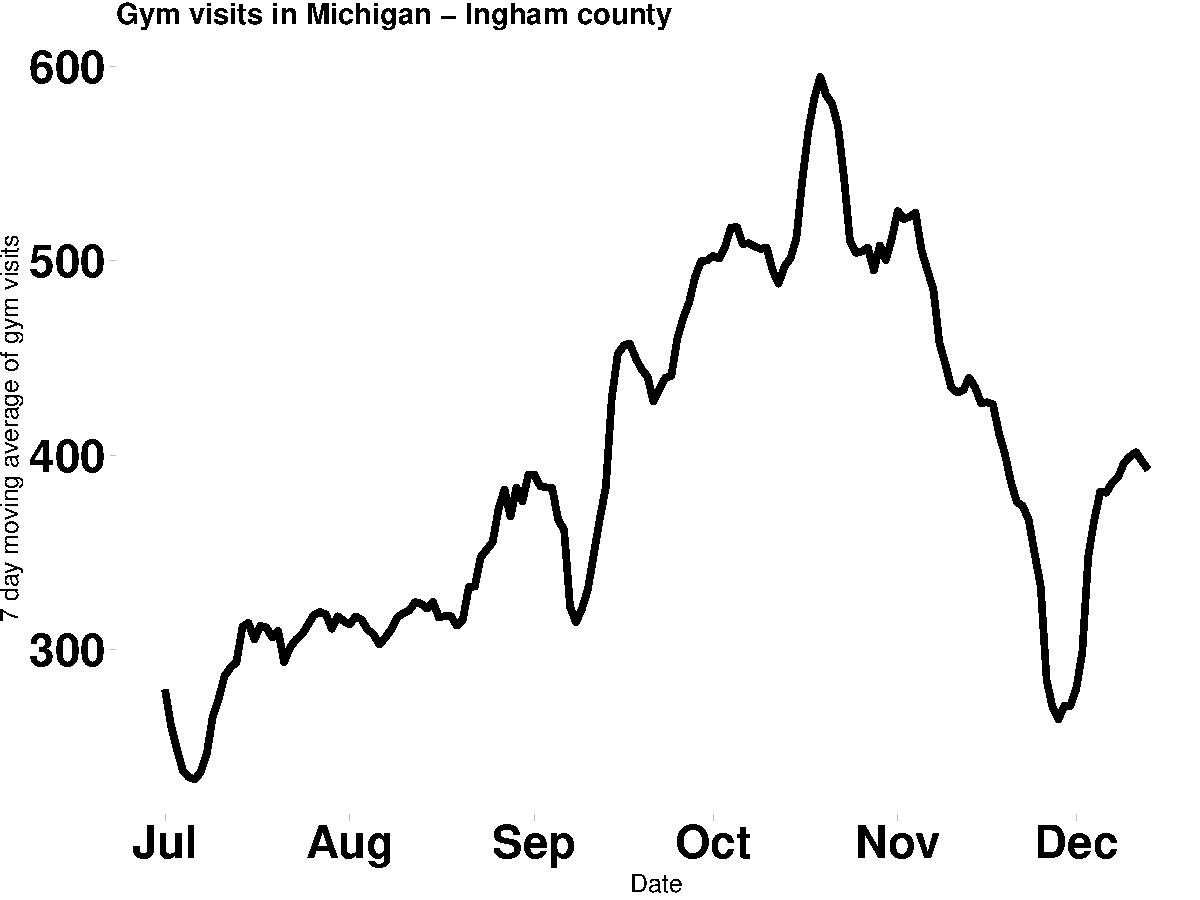
\includegraphics[width=0.20\textwidth]{tables_and_figures/gymMichiganIngham}&
      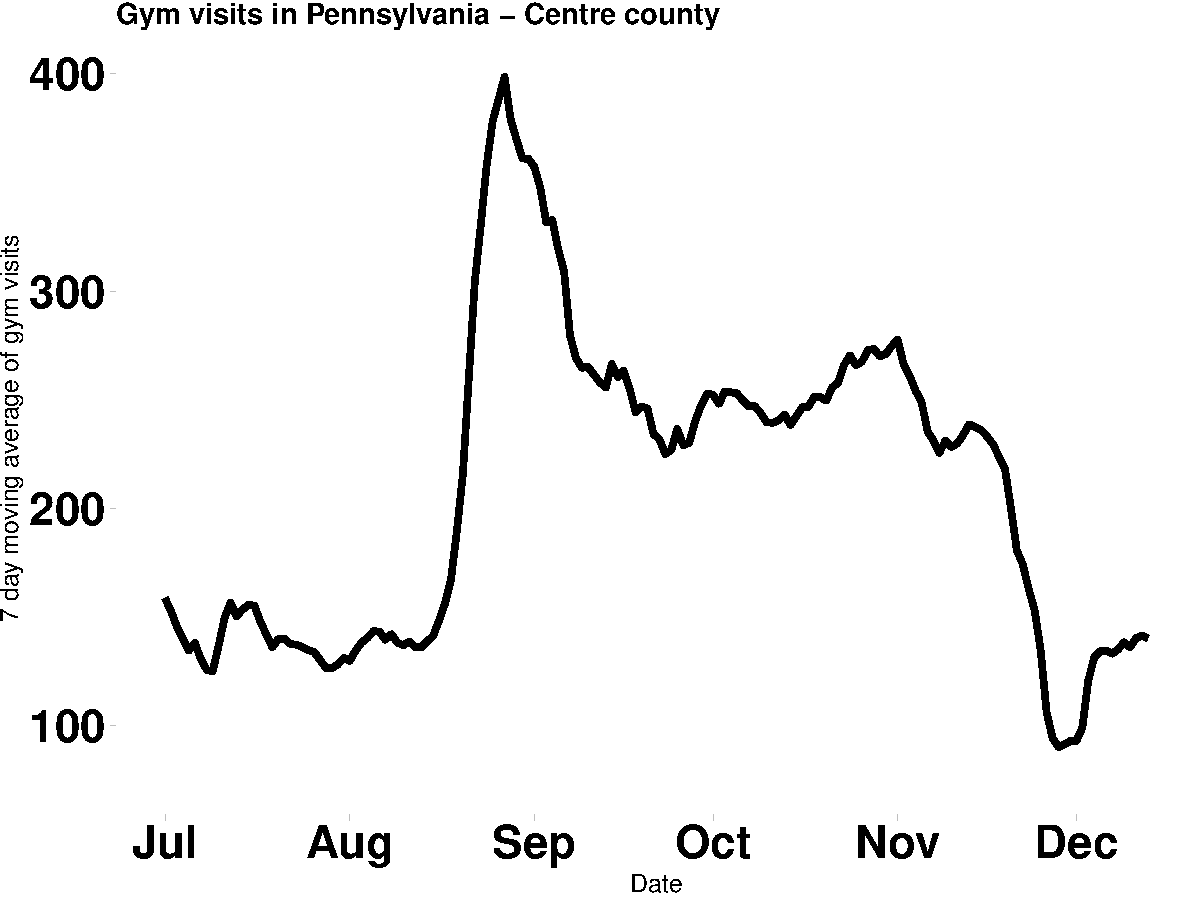
\includegraphics[width=0.20\textwidth]{tables_and_figures/gymPennsylvaniaCentre}&
      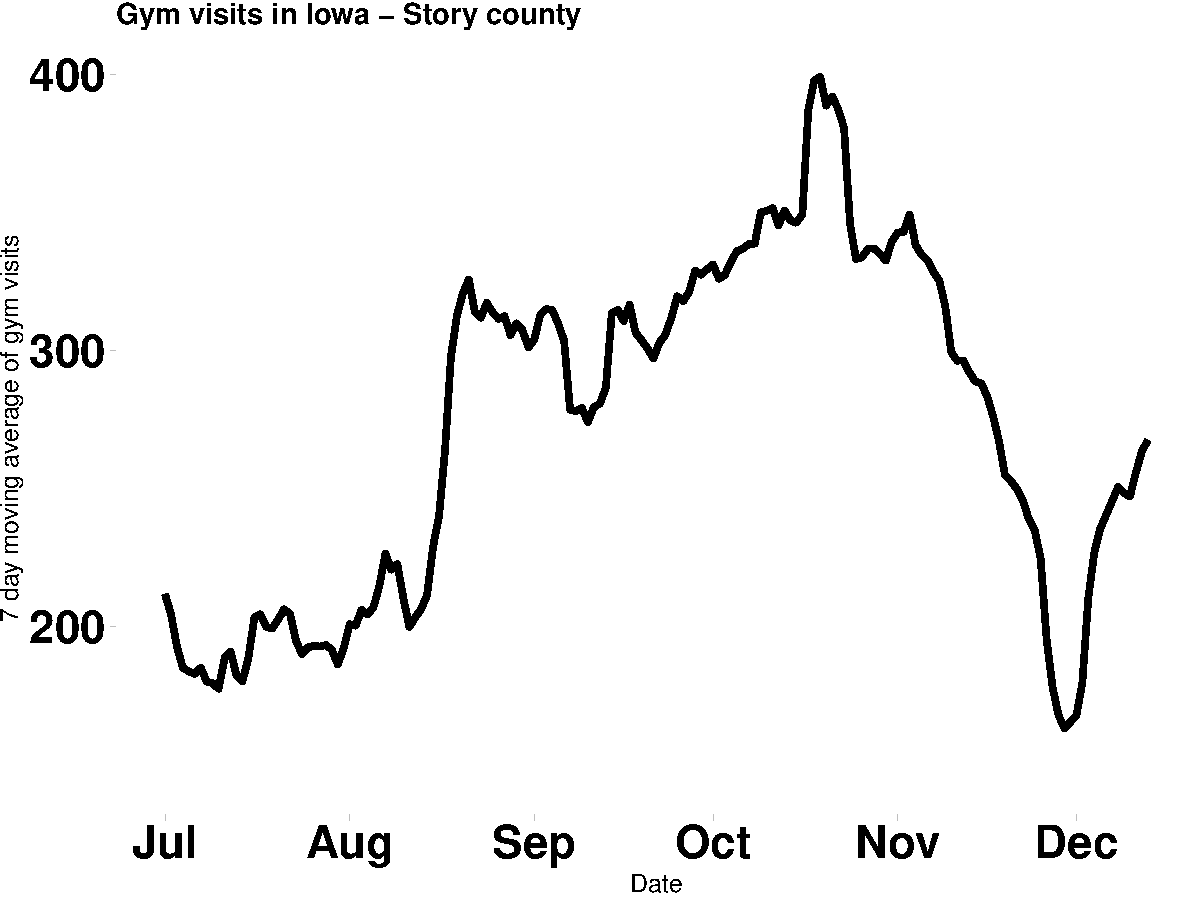
\includegraphics[width=0.20\textwidth]{tables_and_figures/gymIowaStory}& 
      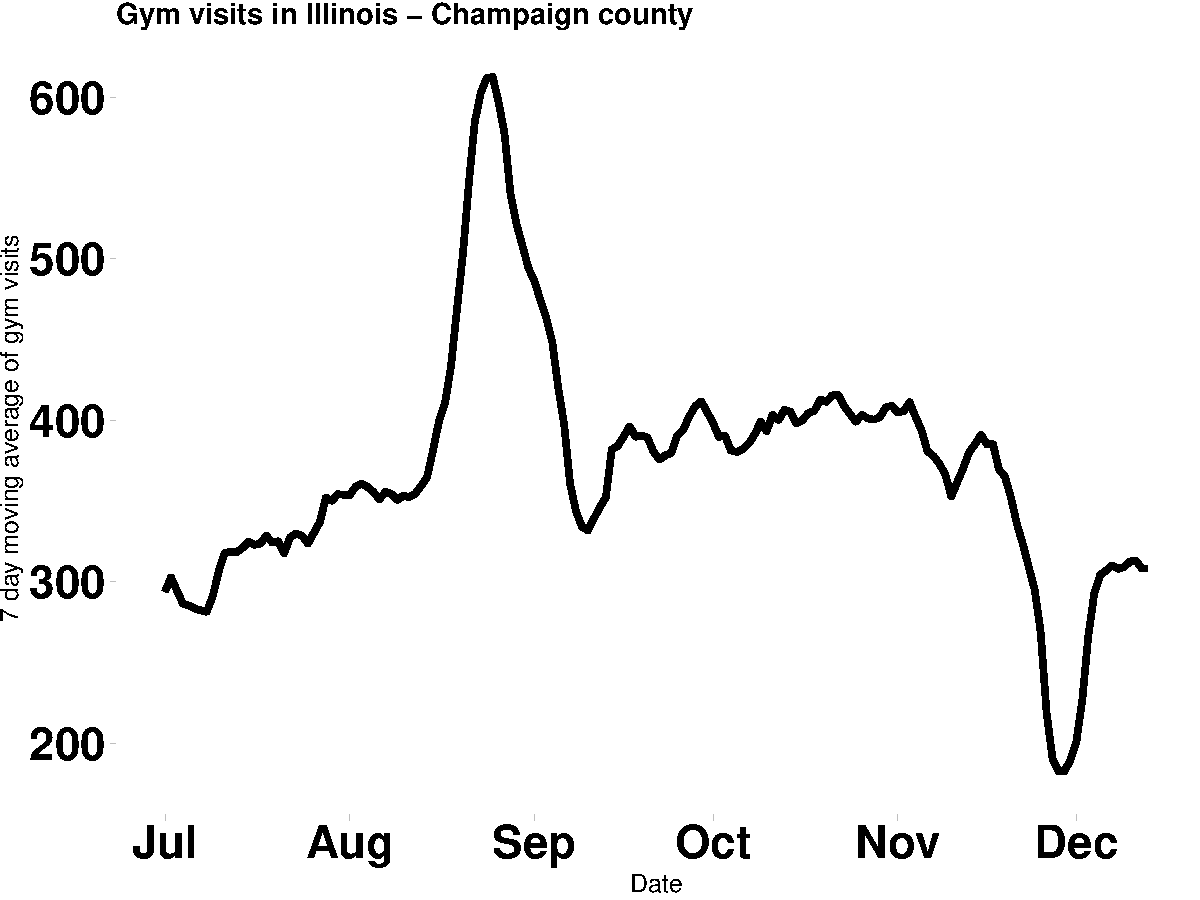
\includegraphics[width=0.20\textwidth]{tables_and_figures/gymIllinoisChampaign}\\   
   School Visits  &  School Visits &School Visits  &  School Visits &School Visits   \\  
      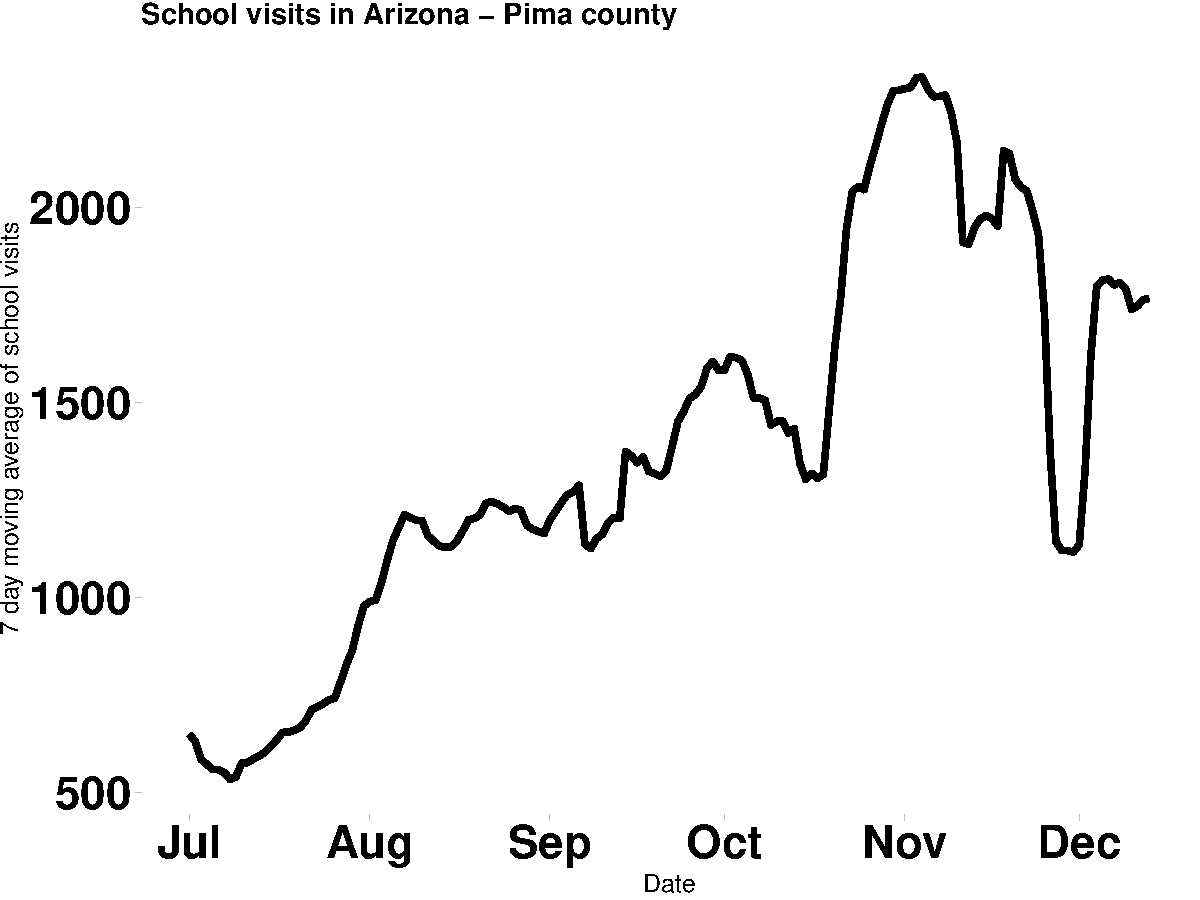
\includegraphics[width=0.20\textwidth]{tables_and_figures/schoolArizonaPima}&
      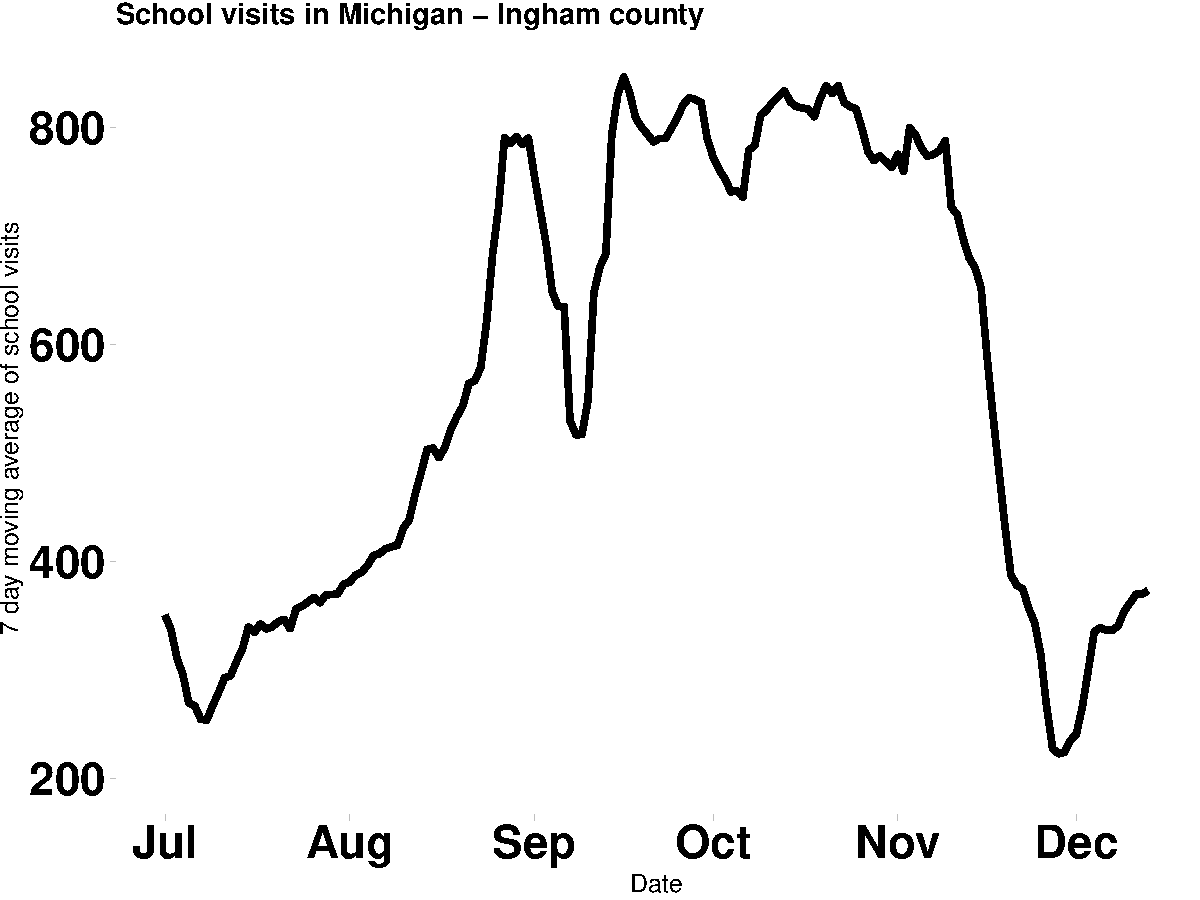
\includegraphics[width=0.20\textwidth]{tables_and_figures/schoolMichiganIngham}&
      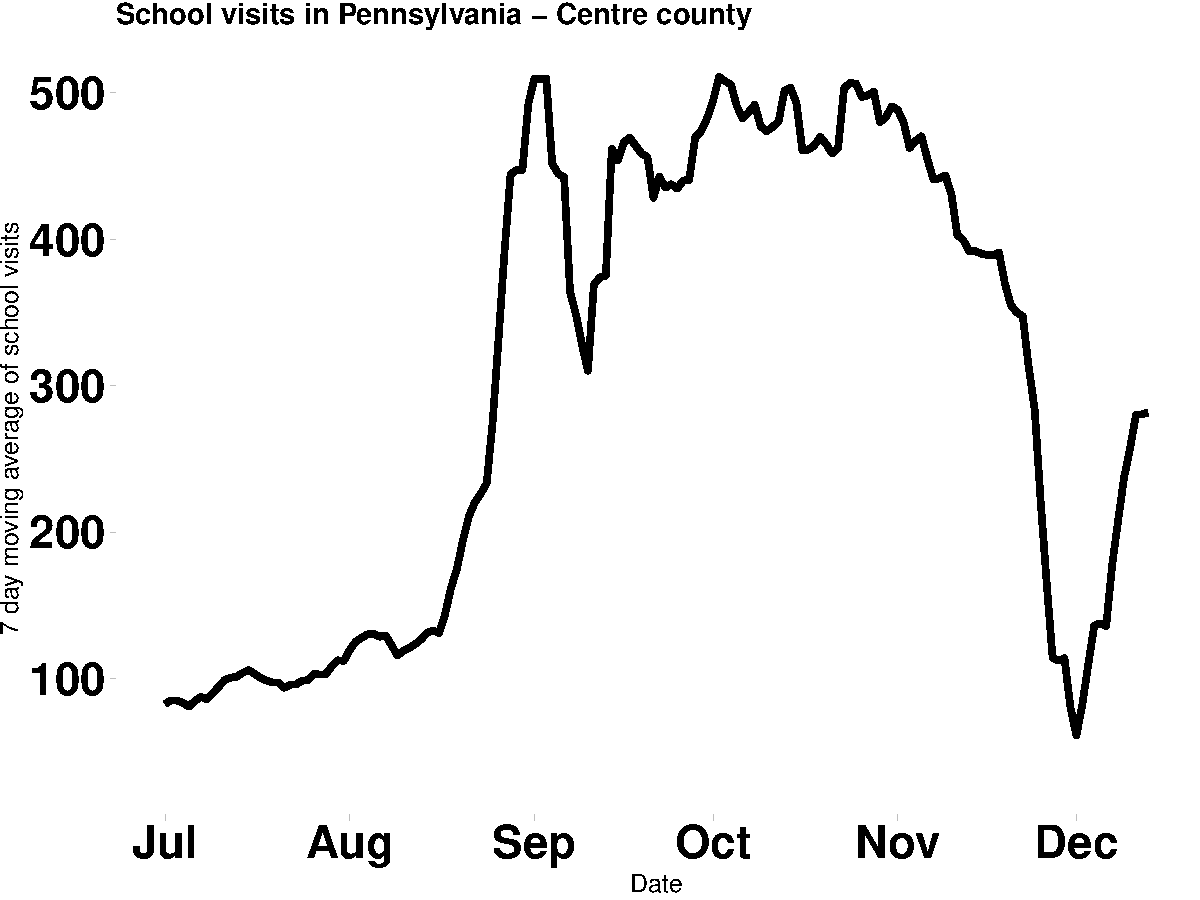
\includegraphics[width=0.20\textwidth]{tables_and_figures/schoolPennsylvaniaCentre}&
      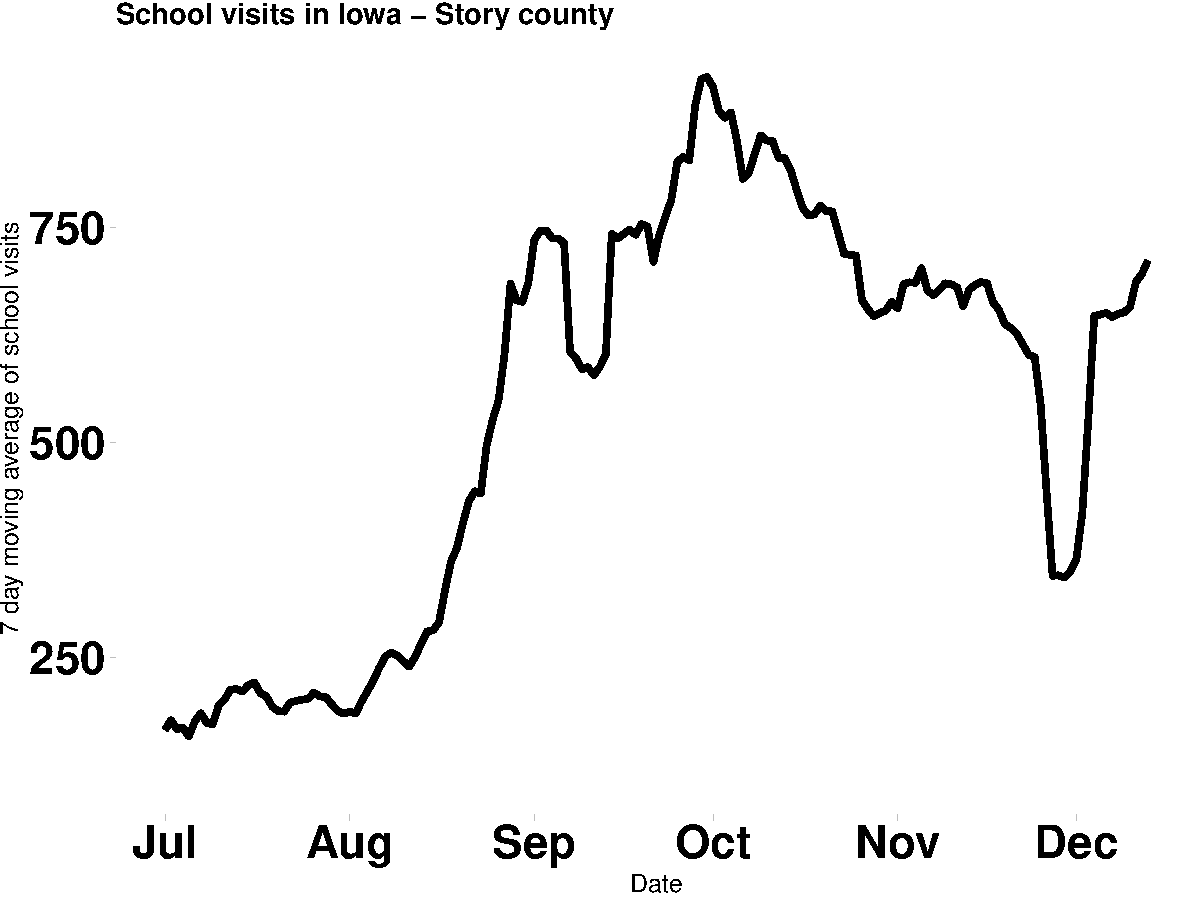
\includegraphics[width=0.20\textwidth]{tables_and_figures/schoolIowaStory}& 
      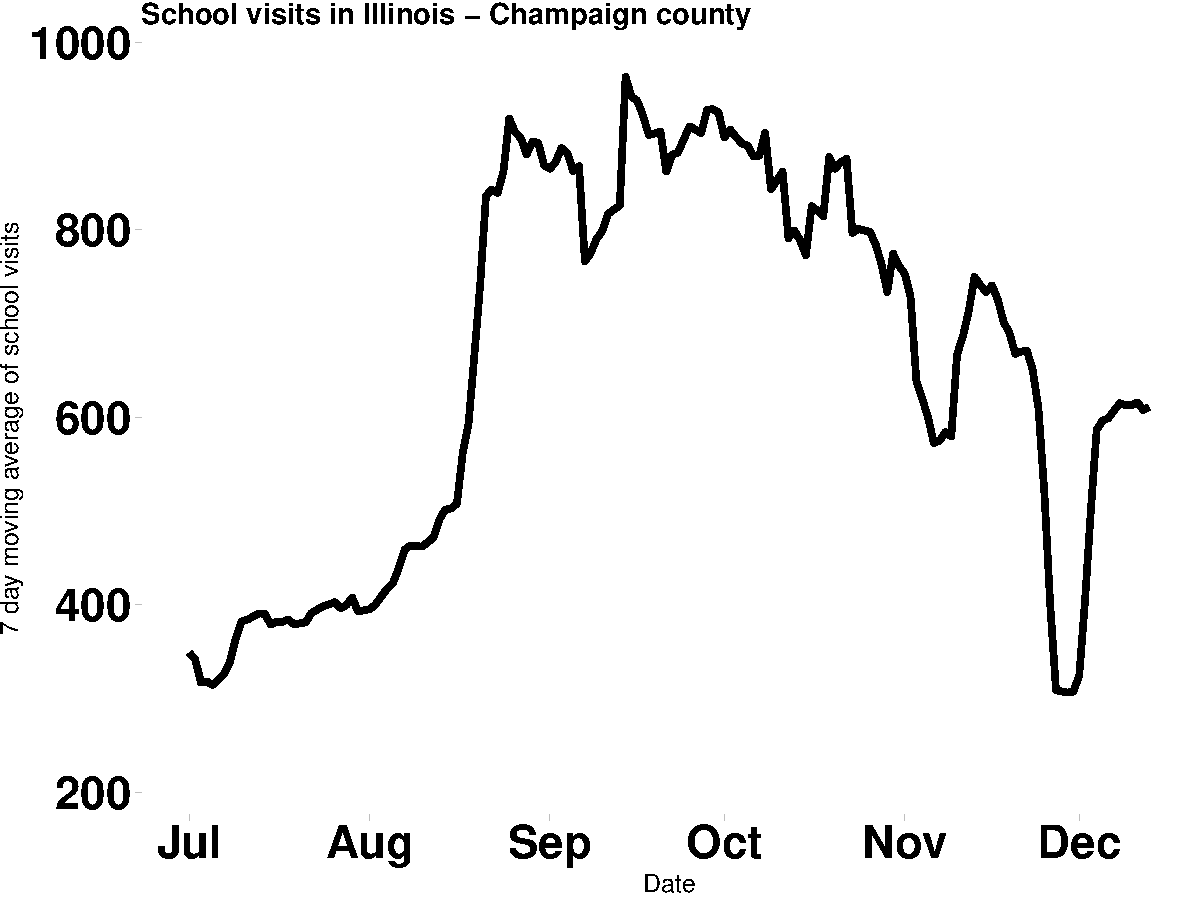
\includegraphics[width=0.20\textwidth]{tables_and_figures/schoolIllinoisChampaign}\\    
   CDC vs. NYT  Cases &  CDC vs. NYT  Cases & CDC vs. NYT  Cases &  CDC vs. NYT  Cases& CDC vs. NYT  Cases  \\ 
          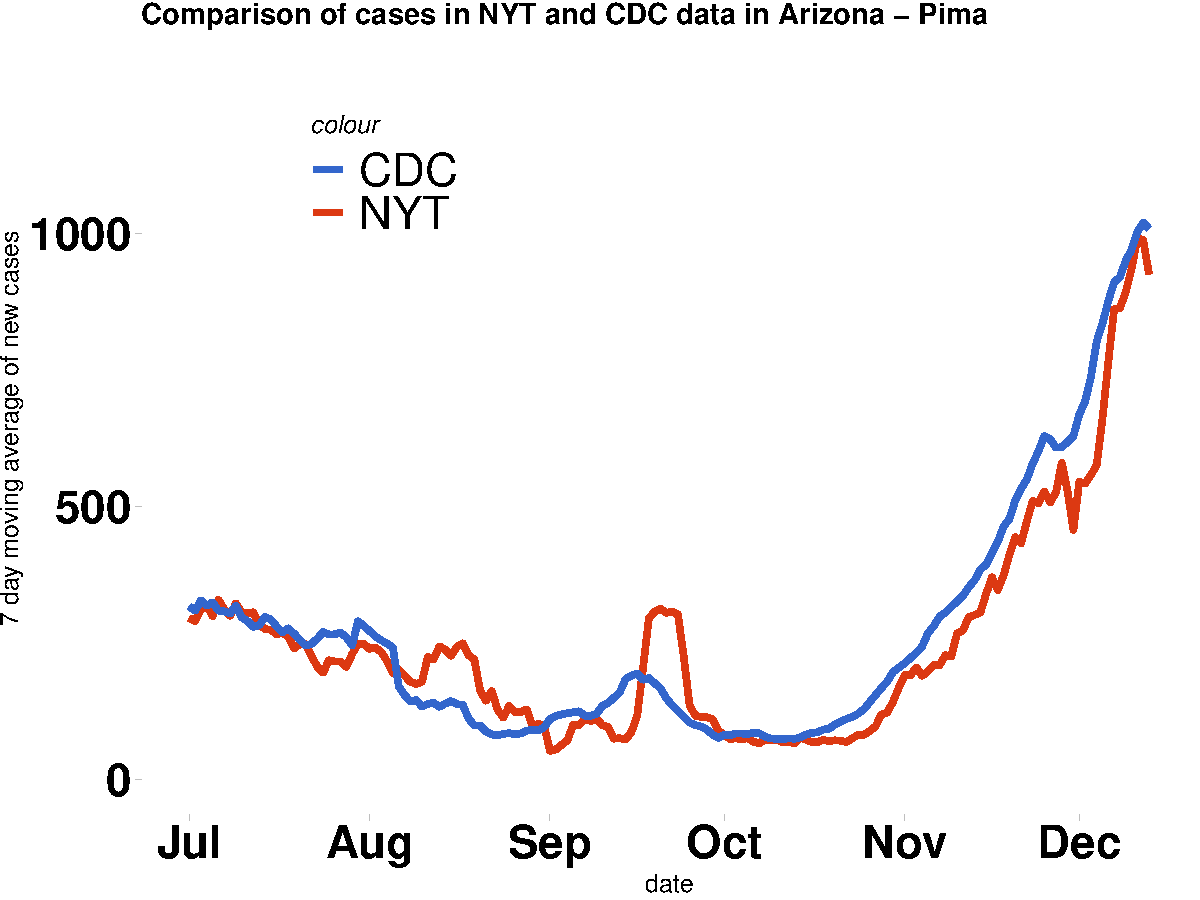
\includegraphics[width=0.20\textwidth]{tables_and_figures/churchArizonaPima}&
      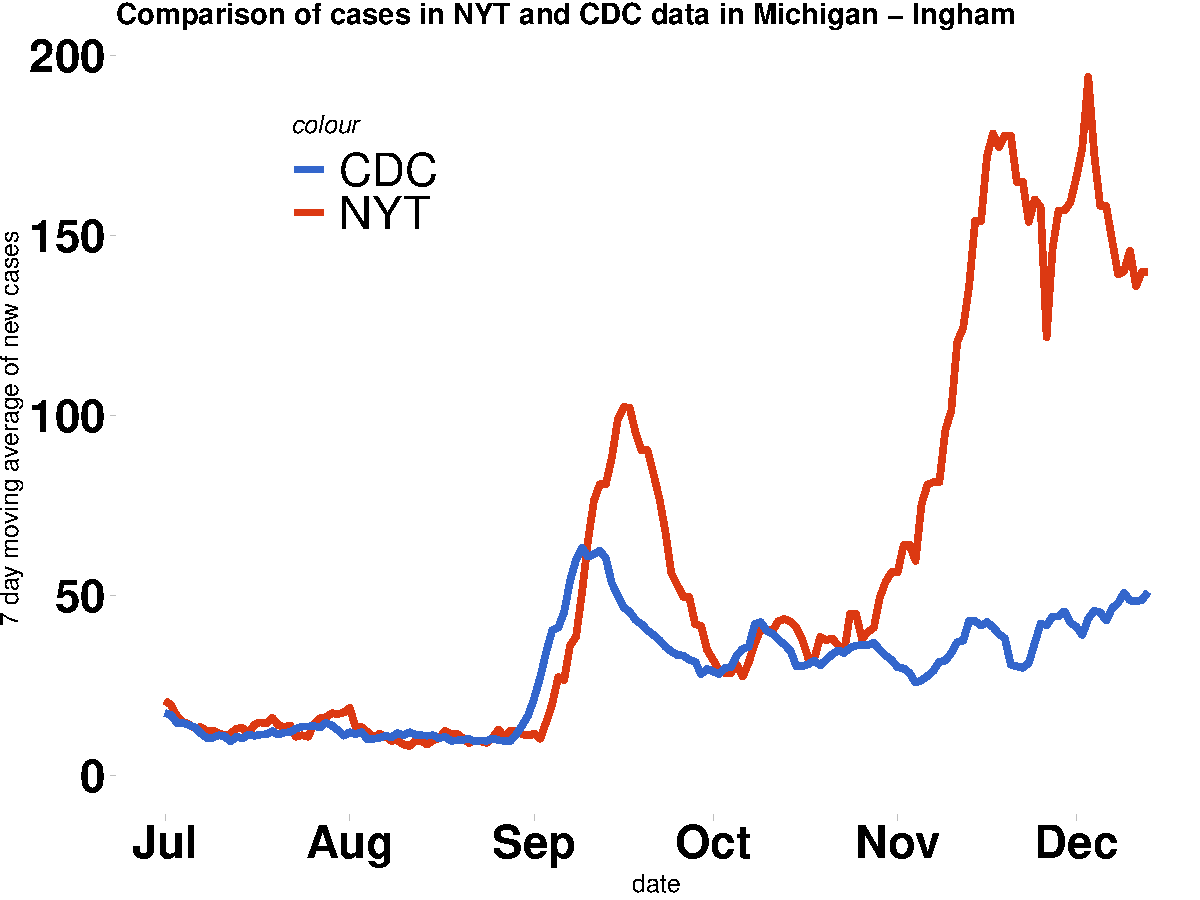
\includegraphics[width=0.20\textwidth]{tables_and_figures/churchMichiganIngham}&
      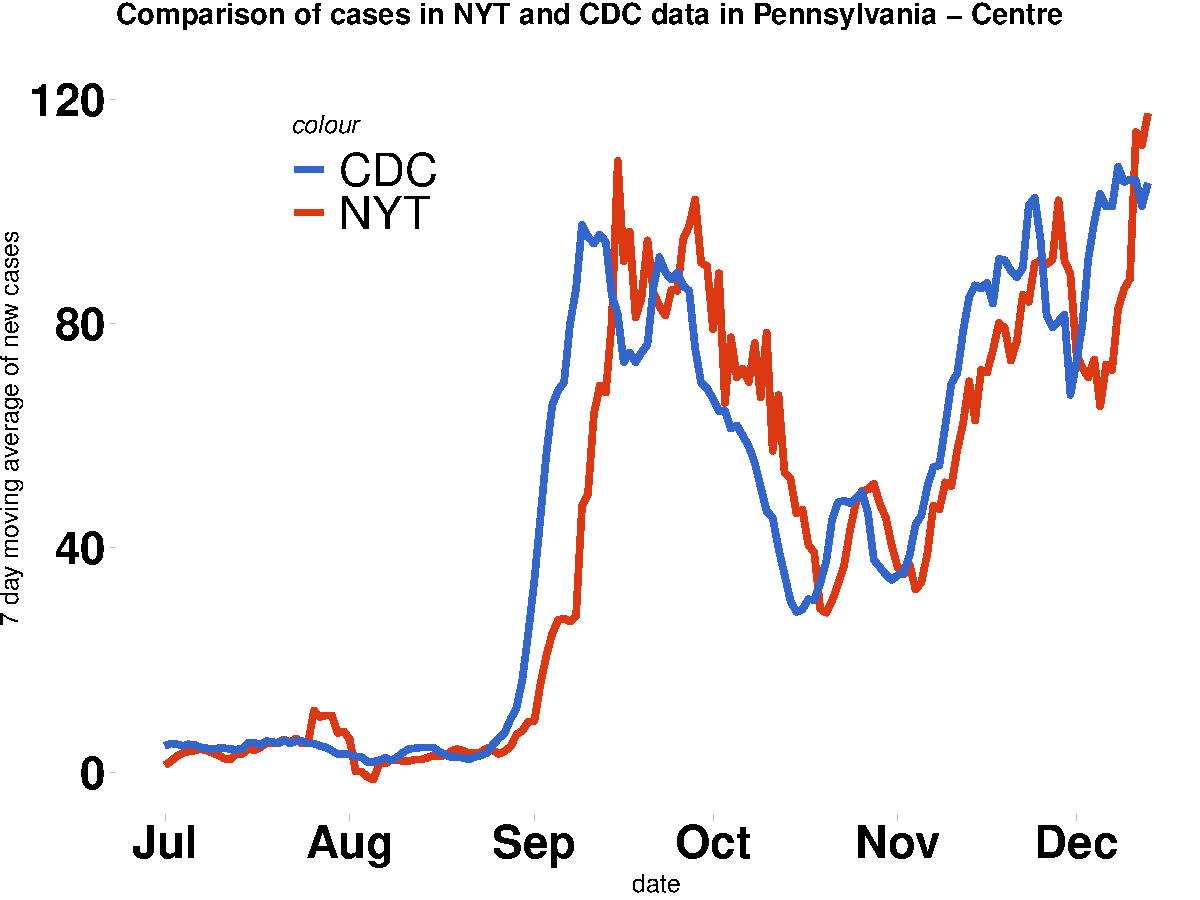
\includegraphics[width=0.20\textwidth]{tables_and_figures/churchPennsylvaniaCentre}&
      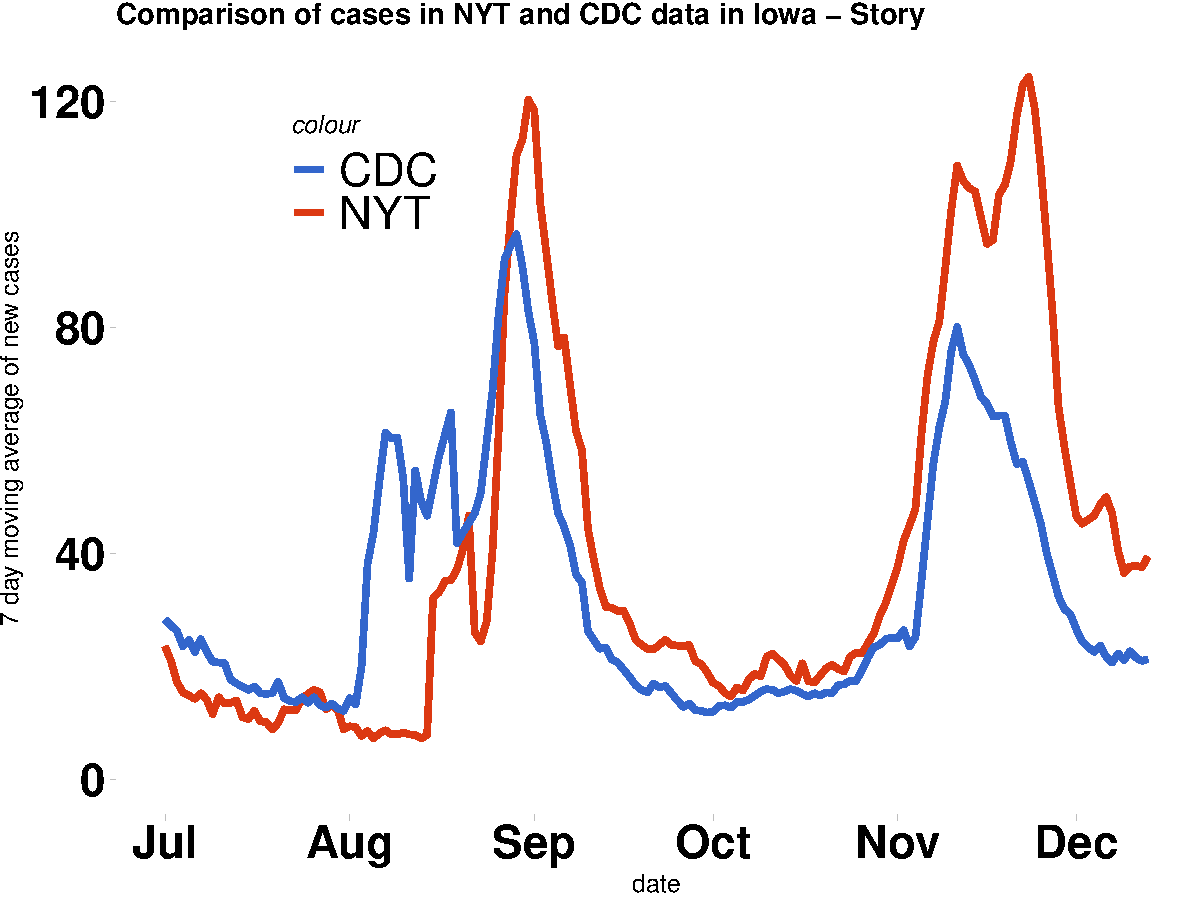
\includegraphics[width=0.20\textwidth]{tables_and_figures/churchIowaStory}& 
      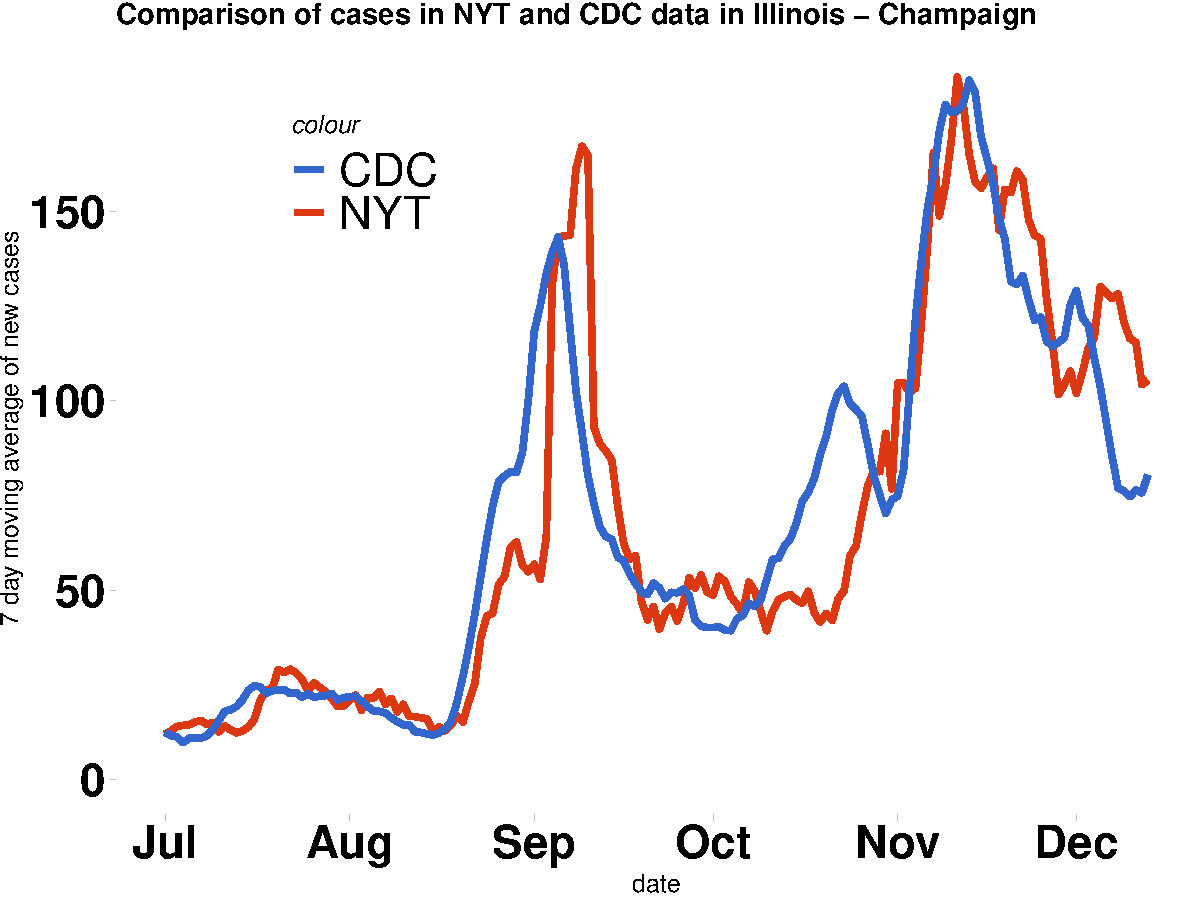
\includegraphics[width=0.20\textwidth]{tables_and_figures/churchIllinoisChampaign}\\     
    \end{tabular} 
  \end{minipage}}  
   {\scriptsize
\begin{flushleft}
Notes: Figure corresponds to Fig. S2 but for Pima, AZ, Ingham, MI, Centre, PA, Story, IA, and Champaign, IL. Across various counties, we also report the evolution of visits to recreation facilities and K-12 school visits. The last panel at the bottom compares the sum of  weekly cases across all age groups reported in CDC dataset with the weekly reported case in NYT dataset.
\end{flushleft}  } 
 \end{figure}




\begin{figure}[!ht] 
\caption{Evolution of Cases/Deaths per 1000 Persons,  Case/Death Growth, Visits to K-12 Schools, Colleges, Restaurants, Bars, Recreational Facilities,   Churches, K-12 School Opening Modes, and NPIs  across U.S. counties \label{fig:evolution-SI}}
\resizebox{0.99\columnwidth}{!}{
\begin{minipage}{\linewidth}
    \centering
        \begin{tabular}{ccc} 
   (a) Wkly Case Growth &  (b)  Wkly Cases per 1000&  (c) Visits to K-12 Schools \\
      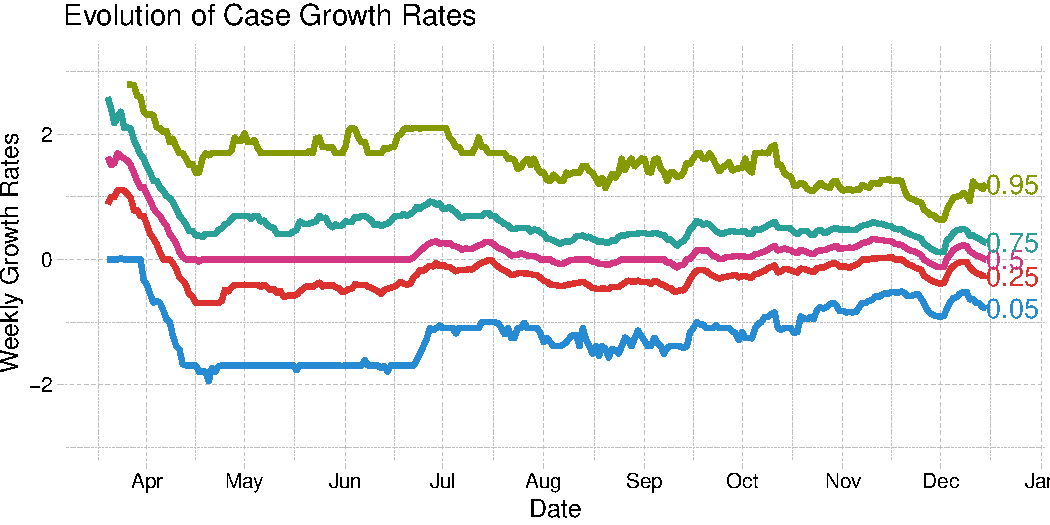
\includegraphics[width=0.33\textwidth]{tables_and_figures/nyt-dlogdc}&
      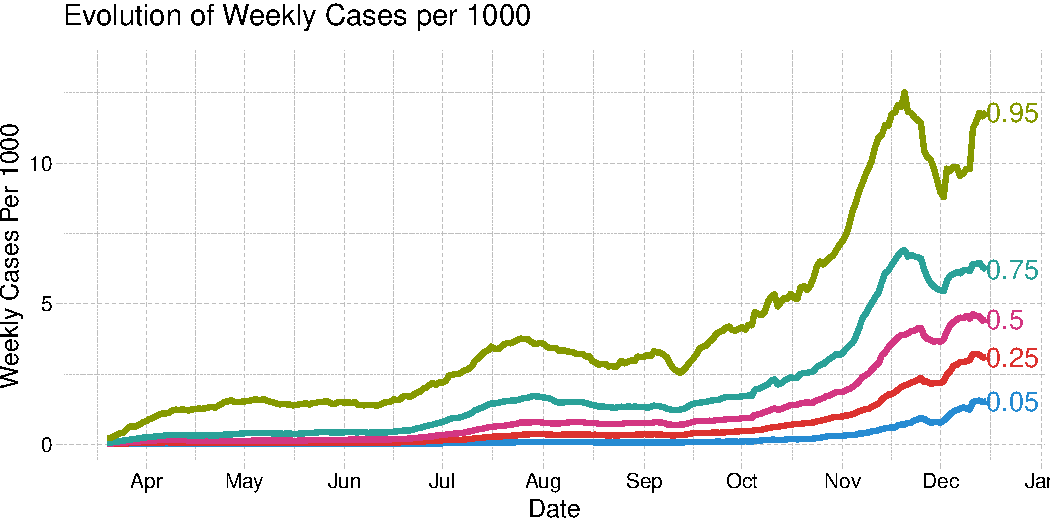
\includegraphics[width=0.33\textwidth]{tables_and_figures/nyt-dcase_capita}&
  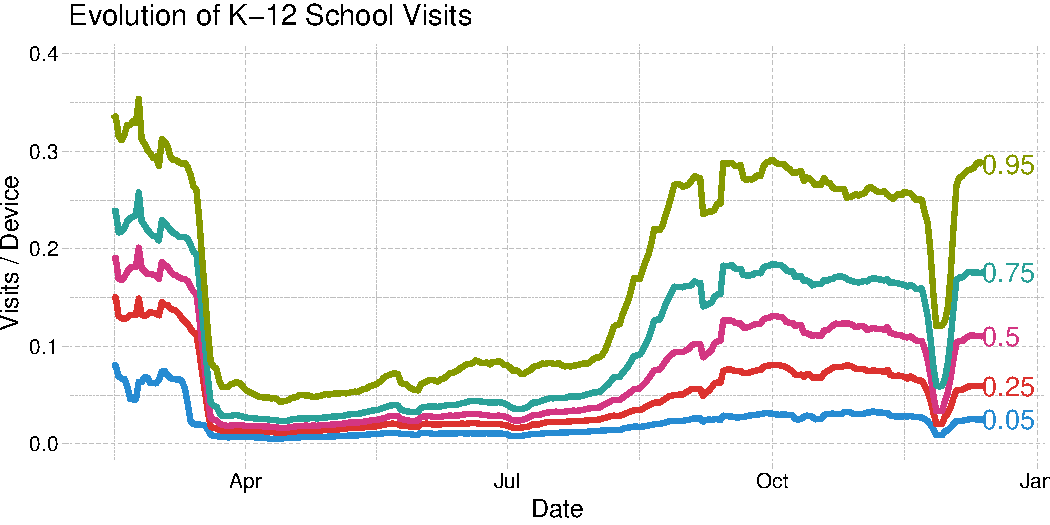
\includegraphics[width=0.33\textwidth]{tables_and_figures/sg-school}\\ 
   (d) Wkly Death Growth &  (e)  Wkly Deaths per 1000 & (f) Visits to Colleges\\
      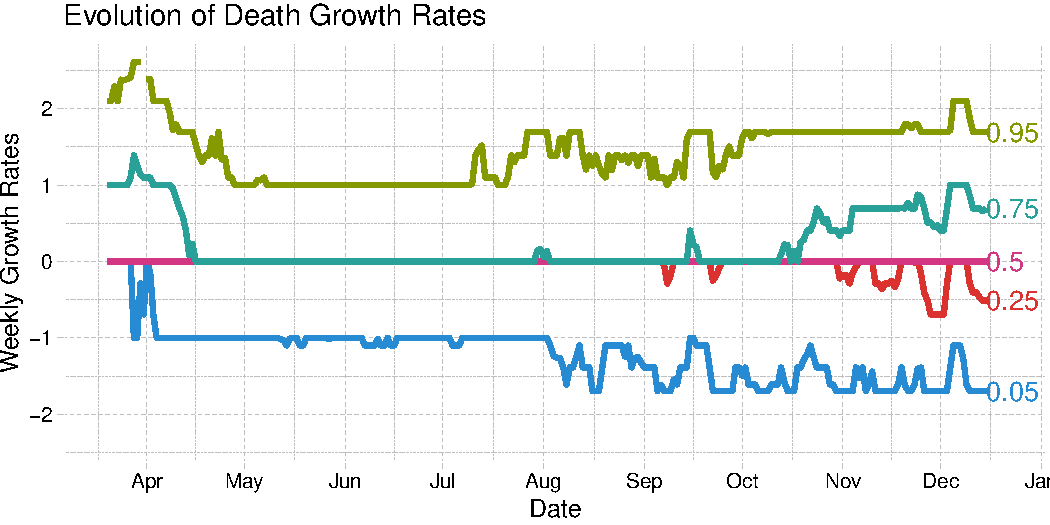
\includegraphics[width=0.33\textwidth]{tables_and_figures/nyt-dlogdd}&
      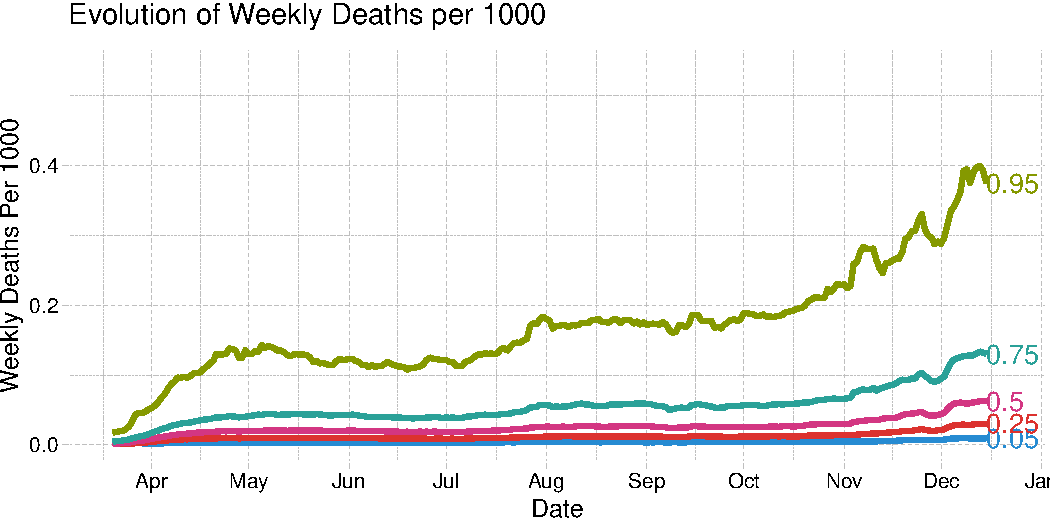
\includegraphics[width=0.33\textwidth]{tables_and_figures/nyt-ddeath_capita}&
  \includegraphics[width=0.33\textwidth]{tables_and_figures/sg-college}\\  
  (g) Visits to Restaurants & (h) Visits to Bars & (i) Visits to Rec. Facilities\\
  \includegraphics[width=0.33\textwidth]{tables_and_figures/sg-restaurant}&
  \includegraphics[width=0.33\textwidth]{tables_and_figures/sg-bar}&
  \includegraphics[width=0.33\textwidth]{tables_and_figures/sg-gym}\\
   (j) Visits to Churches&(k) School Opening Modes & (l) NPIs\\ 
  \includegraphics[width=0.33\textwidth]{tables_and_figures/sg-church}&  \includegraphics[width=0.33\textwidth]{tables_and_figures/ew-opening}&
  \includegraphics[width=0.33\textwidth]{tables_and_figures/jyw-policy}\\
    \end{tabular} 
  \end{minipage}}
  \begin{flushleft}{\ 
Notes:    (a)-(k) report the evolution of various percentiles of corresponding variables in the title over time.  (10)  reports the proportion of counties that open K-12 schools with different teaching methods including ``Unknown'' over time while   (l) reports the proportion of counties that implement three NPIs over time. }
\end{flushleft}   
\end{figure} 



 
 
\begin{table}[!ht] 
\caption{Summary Statistics \label{fig:summary-SI}}
\resizebox{\columnwidth}{!}{
\begin{minipage}{\linewidth}
    \centering
\begin{tabular}{@{\extracolsep{5pt}}lccccccc} 
\\[-1.8ex]\hline 
\hline \\[-1.8ex] 
Statistic & \multicolumn{1}{c}{N} & \multicolumn{1}{c}{Mean} & \multicolumn{1}{c}{St. Dev.} & \multicolumn{1}{c}{Min} & \multicolumn{1}{c}{Pctl(25)} & \multicolumn{1}{c}{Pctl(75)} & \multicolumn{1}{c}{Max} \\ 
\hline \\[-1.8ex] 
Wkly Case Growth Rate over 7 days$^{\text{a}}$& 698,278 & 0.099 & 0.901 & $-$8.107 & $-$0.288 & 0.495 & 8.002 \\ 
Wkly Death Growth Rate over 7 days$^{\text{b}}$ & 698,278 & 0.023 & 0.790 & $-$6.170 & 0.000 & 0.000 & 6.170 \\ 
Wkly Death Growth Rate over 21 days$^{\text{c}}$ & 633,617 & 0.115 & 0.988 & $-$5.159 & $-$0.211 & 0.693 & 5.277 \\ 
log(Wkly Cases)$^{\text{d}}$  & 703,702 & 2.829 & 2.140 & $-$1.000 & 1.386 & 4.331 & 10.488 \\ 
log(Wkly Deaths)$^{\text{e}}$& 703,702 & $-$0.269 & 1.147 & $-$1.000 & $-$1.000 & 0.000 & 6.479 \\ 
College Visits  & 728,228 & 0.010 & 0.031 & 0.000 & 0.000 & 0.008 & 1.827 \\ 
K-12 School Visits   & 728,228 & 0.074 & 0.072 & 0.000 & 0.024 & 0.103 & 1.167 \\ 
K-12 opening, in-person& 646,816 & 0.079 & 0.207 & 0.000 & 0.000 & 0.000 & 1.000 \\ 
K-12 opening, Hybrid & 646,816 & 0.224 & 0.357 & 0.000 & 0.000 & 0.424 & 1.000 \\ 
K-12 opening, Remote& 646,816 & 0.078 & 0.227 & 0.000 & 0.000 & 0.000 & 1.000 \\ 
No-Mask for Staffs & 577,680 & 0.293 & 0.455 & 0.000 & 0.000 & 1.000 & 1.000 \\ 
Mandatory Mask & 728,944 & 0.461 & 0.495 & 0 & 0 & 1 & 1 \\ 
Ban Gathering & 728,944 & 0.658 & 0.472 & 0 & 0 & 1 & 1 \\ 
Stay at Home & 728,944 & 0.143 & 0.345 & 0 & 0 & 0 & 1 \\ 
Full Time Workplace Visits  & 728,206 & 0.054 & 0.018 & 0.010 & 0.042 & 0.061 & 0.484 \\ 
Part Time Workplace Visits & 728,206 & 0.101 & 0.025 & 0.023 & 0.084 & 0.113 & 0.567 \\ 
Staying Home Devices & 728,206 & 0.342 & 0.116 & 0.021 & 0.267 & 0.393 & 3.657 \\ 
Recreational Place Visits & 728,228 & 0.017 & 0.022 & 0.000 & 0.000 & 0.026 & 0.786 \\ 
Church Visits & 728,228 & 0.025 & 0.018 & 0.000 & 0.014 & 0.032 & 0.583 \\ 
Drinking Place Visits & 728,228 & 0.012 & 0.024 & 0.000 & 0.0001 & 0.015 & 1.461 \\ 
Restaurant Visits & 728,228 & 0.250 & 0.175 & 0.000 & 0.150 & 0.315 & 4.261 \\ 
Test Growth Rates& 698,278 & 0.067 & 1.099 & $-$13.616 & $-$0.051 & 0.178 & 13.111 \\ 
Population in 2018 (millions) & 706,966 & 0.104 & 0.331 & 0.0002 & 0.012 & 0.071 & 10.106 \\ 
 \hline \\[-1.8ex] 
\end{tabular} 
  {\scriptsize
\begin{flushleft}
Notes:  Based on observations from April 15, 2020 to December 2, 2020 for the maximum of 3142 counties. The growth rates of weekly reported cases/deaths over 7 days are measured by the log-difference over 7 days in weekly cases/deaths in (a) and (b) while the growth rates of weekly deaths over 21 days is measured by the log-difference over 21 days in weekly cases/deaths in (c). For (a)-(e),  the log of weekly cases and deaths is set to be $-1$ when we observe zero weekly cases and deaths. 
\end{flushleft}}   
 \end{minipage}}
\end{table}


   
 
\begin{table}[ht] 
\caption{Correlation across variables  \label{fig:corr-SI}}
\resizebox{0.9\columnwidth}{!}{
\begin{minipage}{\linewidth}
    \centering
\begin{tabular}{lcccccccccccccccc}
\toprule
\rotatebox{90}{ } & \rotatebox{90}{College Visits} & \rotatebox{90}{K-12 School Visits} & \rotatebox{90}{Open K-12 In-person} & \rotatebox{90}{Open K-12 Hybrid} & \rotatebox{90}{Open K-12 Remote} & \rotatebox{90}{No-Mask for Staffs} & \rotatebox{90}{Mandatory mask} & \rotatebox{90}{Ban gatherings} & \rotatebox{90}{Stay at home} & \rotatebox{90}{Full-time Workplace Visits} & \rotatebox{90}{Part-time Workplace Visits} & \rotatebox{90}{Staying Home Devices} & \rotatebox{90}{Bar Visits} & \rotatebox{90}{Restaurant Visits} & \rotatebox{90}{Rec. Facilities Visits} & \rotatebox{90}{Church Vists}\\
\midrule
College Visits & 1.00 &  &  &  &  &  &  &  &  &  &  &  &  &  &  & \\
K-12 School Visits & 0.09 & 1.00 &  &  &  &  &  &  &  &  &  &  &  &  &  & \\
Open K-12 In-person & 0.05 & 0.43 & 1.00 &  &  &  &  &  &  &  &  &  &  &  &  & \\
Open K-12 Hybrid & 0.11 & 0.44 & 0.04 & 1.00 &  &  &  &  &  &  &  &  &  &  &  & \\
Open K-12 Remote & 0.05 & 0.09 & -0.06 & -0.06 & 1.00 &  &  &  &  &  &  &  &  &  &  & \\
\addlinespace
No-Mask for Staffs & 0.01 & 0.16 & 0.15 & -0.02 & -0.10 & 1.00 &  &  &  &  &  &  &  &  &  & \\
Mandatory mask & 0.09 & 0.10 & 0.03 & 0.24 & 0.23 & -0.31 & 1.00 &  &  &  &  &  &  &  &  & \\
Ban gatherings & -0.03 & -0.14 & -0.09 & -0.06 & 0.00 & -0.03 & -0.09 & 1.00 &  &  &  &  &  &  &  & \\
Stay at home & -0.06 & -0.24 & -0.14 & -0.21 & -0.13 & -0.08 & -0.19 & 0.20 & 1.00 &  &  &  &  &  &  & \\
Full-time Workplace Visits & 0.04 & 0.56 & 0.37 & 0.36 & 0.10 & 0.12 & 0.05 & -0.17 & -0.21 & 1.00 &  &  &  &  &  & \\
\addlinespace
Part-time Workplace Visits & 0.06 & 0.60 & 0.32 & 0.34 & 0.04 & 0.20 & -0.01 & -0.12 & -0.31 & 0.71 & 1.00 &  &  &  &  & \\
Staying Home Devices & -0.04 & -0.27 & -0.18 & -0.23 & -0.02 & -0.10 & 0.01 & -0.00 & 0.27 & 0.06 & -0.19 & 1.00 &  &  &  & \\
Bar Visits & 0.05 & 0.08 & 0.02 & -0.02 & 0.01 & 0.08 & 0.01 & -0.06 & -0.08 & 0.12 & 0.11 & 0.15 & 1.00 &  &  & \\
Restaurant Visits & 0.17 & 0.02 & -0.10 & 0.00 & 0.06 & -0.10 & 0.14 & 0.10 & -0.08 & -0.07 & 0.07 & 0.04 & 0.34 & 1.00 &  & \\
Rec. Facilities Visits & 0.15 & -0.00 & -0.07 & 0.03 & 0.11 & -0.08 & 0.18 & 0.03 & -0.08 & -0.05 & -0.03 & 0.09 & 0.26 & 0.52 & 1.00 & \\
\addlinespace
Church Vists & 0.06 & 0.32 & 0.13 & 0.08 & -0.03 & 0.17 & -0.06 & -0.07 & -0.16 & 0.15 & 0.37 & -0.18 & 0.11 & 0.18 & 0.03 & 1.00\\
\bottomrule
\end{tabular} {\scriptsize
\begin{flushleft}
Notes:  Based on observations from April 15, 2020 to December 2, 2020 for the maximum of 3142 counties. \end{flushleft}}   
 \end{minipage}}
\end{table}

\begin{table}[ht] 
\caption{Correlation across mitigation variables  \label{fig:corr-mitigation}}
%\resizebox{0.9\columnwidth}{!}{
%\begin{minipage}{\linewidth}
    \centering
\begin{tabular}{lcccc}
\rotatebox{90}{ } & \rotatebox{90}{\parbox{1.5cm}{No mask\\ for staffs}} & \rotatebox{90}{\parbox{1.5cm}{No mask\\ for students}} & \rotatebox{90}{\parbox{1.5cm}{Yes sports \\for students}} & \rotatebox{90}{\parbox{1.5cm}{No online \\instruction}}\\
\midrule
No mask for staffs & 1.00 &  &  & \\
No mask for students & 0.74$^{***}$ & 1.00 &  & \\
Yes sports for students & 0.14$^{***}$  & 0.07$^{***}$  & 1.00 & \\
No online instruction & 0.13$^{***}$ & 0.12$^{***} $ & 0.06$^{**}$  & 1.00\\
\bottomrule
\end{tabular} {\scriptsize
\begin{flushleft}
Notes:  Based on cross-sectional observations on October 1, 2020.  $^{**}$p$<$0.05; $^{***}$p$<$0.01
 \end{flushleft}}
% \end{minipage}
 %}
\end{table}  
 
%\section*{Figures}

\begin{figure}[ht]
  \caption{Average weekly cases and deaths are associated with different modes of opening K-12 schools,  visits to K-12 schools, and visits to colleges/universities \label{fig:case-growth-SI}}  
\resizebox{0.87\columnwidth}{!}{
\begin{minipage}{\linewidth} 
        \begin{tabular}{cccc}  
%    (a)  Cases by K-12 Opening Modes & (b) Deaths by  K-12 Opening Modes \\
%      \includegraphics[width=0.50\textwidth]{tables_and_figures/schoolmode-event-newcases}&  
%      \includegraphics[width=0.50\textwidth]{tables_and_figures/schoolmode-event-newdeaths}\\ 
%   (c) K-12 Visits  by  Opening Modes &  (d)  Cases by K-12 Visits\\
%  \includegraphics[width=0.50\textwidth]{tables_and_figures/schoolmode-event-visits}&
%  \includegraphics[width=0.50\textwidth]{tables_and_figures/school-weekcase-simple}\\ 
%      (e) Cases by  College Visits  & (f) Deaths by College Visits\\ 
%         \includegraphics[width=0.50\textwidth]{tables_and_figures/college-weekcase-simple}& 
%         \includegraphics[width=0.50\textwidth]{tables_and_figures/college-weekdeath-simple} \\
%   (a)  Cases by Opening Modes (Trump>Med)  & (b) Cases by  Opening Modes (Trump<=Med) &  (c)  Cases by Opening Modes (Mask<=Med)  & (d) Cases by  Opening Modes (Mask>Med)\\ 
%  \includegraphics[width=0.25\textwidth]{tables_and_figures/schoolmode-event-newcases-trump}&
%  \includegraphics[width=0.25\textwidth]{tables_and_figures/schoolmode-event-newcases-notrump} &  \includegraphics[width=0.25\textwidth]{tables_and_figures/schoolmode-event-newcases-mask}&
%  \includegraphics[width=0.25\textwidth]{tables_and_figures/schoolmode-event-newcases-nomask} \\
  \textbf{(a) K-12 School Visits}   &   \textbf{(b) Restaurant Visits    } &  \textbf{(c)  Recreation Facilitiy Visits  }  &  \textbf{(d) Church Visits}  \\ %  (h)  Church Visits   \\ 
  \includegraphics[width=0.25\textwidth]{tables_and_figures/schoolmode-event-school.pdf}&
  \includegraphics[width=0.25\textwidth]{tables_and_figures/schoolmode-event-restaurant}&  
  \includegraphics[width=0.25\textwidth]{tables_and_figures/schoolmode-event-recreation}&  
  \includegraphics[width=0.25\textwidth]{tables_and_figures/schoolmode-event-church}\\  
    \textbf{(e) Full-Time Workplace Visits  }&\textbf{(f) Part-Time Workplace Visits     }&\textbf{(g) Staying Home Devices }&\textbf{(h) Bar Visits } \\ %  (h)  Church Visits   \\ 
  \includegraphics[width=0.25\textwidth]{tables_and_figures/schoolmode-event-fullwork}&
  \includegraphics[width=0.25\textwidth]{tables_and_figures/schoolmode-event-partwork}&  
  \includegraphics[width=0.25\textwidth]{tables_and_figures/schoolmode-event-home}&  
  \includegraphics[width=0.25\textwidth]{tables_and_figures/schoolmode-event-bar}\\  
      \textbf{(i)     Cases by  Opening Modes }&\textbf{(j) Cases by  Opening Modes }&\textbf{(k) Cases by  Opening Modes}&\textbf{(l) Cases by  Opening Modes }\\
    (Student Mask Requirements)&(Staff Mask Requirements)&   (Sports Activities)&   (Online Instruction Increase) \\  
      \includegraphics[width=0.25\textwidth]{tables_and_figures/schoolmode-event-newcases}&  
      \includegraphics[width=0.25\textwidth]{tables_and_figures/schoolmode-event-staff-newcases}&  
      \includegraphics[width=0.25\textwidth]{tables_and_figures/schoolmode-event-sports-newcases}&  
      \includegraphics[width=0.25\textwidth]{tables_and_figures/schoolmode-event-online-newcases}  \\
    \textbf{(m)   Deaths by  Opening Modes }&\textbf{(n) Deaths by  Opening Modes }&\textbf{(o) Deaths by  Opening Modes}&\textbf{(p) Deaths  by  Opening Modes }\\
    (Student Mask Requirements)&(Staff Mask Requirements)&   (Sports Activities)&   (Online Instruction Increase) \\  
          \includegraphics[width=0.25\textwidth]{tables_and_figures/schoolmode-event-newdeaths}&  
      \includegraphics[width=0.25\textwidth]{tables_and_figures/schoolmode-event-staff-newdeaths}&  
      \includegraphics[width=0.25\textwidth]{tables_and_figures/schoolmode-event-sports-newdeaths}&  
      \includegraphics[width=0.25\textwidth]{tables_and_figures/schoolmode-event-online-newdeaths}  \\  
      \textbf{(q) Cases by K-12 Visits }&\textbf{(r) Cases by K-12 Visits }&\textbf{(s) Cases by K-12 Visits }&\textbf{(t) Cases by K-12 Visits } \\
    (Student Mask Requirements)&(Staff Mask Requirements)&   (Sports Activities)&   (Online Instruction Increase) \\  
      \includegraphics[width=0.25\textwidth]{tables_and_figures/school-weekcase-simple}&  
      \includegraphics[width=0.25\textwidth]{tables_and_figures/school-weekcase-staff-simple}&  
      \includegraphics[width=0.25\textwidth]{tables_and_figures/school-weekcase-sports-simple}&  
      \includegraphics[width=0.25\textwidth]{tables_and_figures/school-weekcase-online-simple}  \\
    \textbf{(u)  Deaths by K-12 Visits}  &\textbf{(v) Deaths by K-12 Visits}&\textbf{(w) Deaths by K-12 Visits }&\textbf{(x) Deaths by K-12 Visits}\\
    (Student Mask Requirements)&(Staff Mask Requirements)&   (Sports Activities)&   (Online Instruction Increase) \\  
      \includegraphics[width=0.25\textwidth]{tables_and_figures/school-weekdeath-simple}&  
      \includegraphics[width=0.25\textwidth]{tables_and_figures/school-weekdeath-staff-simple}&  
      \includegraphics[width=0.25\textwidth]{tables_and_figures/school-weekdeath-sports-simple} &  
      \includegraphics[width=0.25\textwidth]{tables_and_figures/school-weekdeath-online-simple}  
    \end{tabular} 
  \end{minipage}}  
\vspace{-0.2cm}  {\scriptsize
\begin{flushleft}

Notes:  (a)-(h)  plot the evolution of corresponding variables in the title before and after the day of school openings and corresponding to figures reported in Fig. 1(c)(d) in the main text. (i)-(p) corresponds to Fig.(a)(b) and  plot the evolution of weekly cases or deaths per 1000 persons averaged across counties within each group of counties classified by K-12 school teaching methods and different mitigation strategies (mask requirements for students, mask requirements for staffs, allowing for sports activities, and increase in online instructions) against the days since K-12 school opening. In (i) and (m), counties that implement in-person teaching  are classified into ``In-person/Yes-Mask" and  ``In-person/No-Mask" based on whether at least one school district requires students to wear masks or not. In (k) and (o),  counties that implement in-person teaching are classified into ``In-person/Yes-Sports" and  ``In-person/No-Sports" based on whether at least one school district requires students to allow sports activities or not. In (l) and (p),  counties that implement in-person teaching   are classified into ``In-person/No-Online" and  ``In-person/Yes-Online" based on whether at least one school district answer that no increase in online instruction. (q)-(x) are similar to (i)-(p) but classify counties by the volume of per-device K-12 school visits and take the calendar dates instead of the days since opening schools as x-axis, where  "Low,"   "Middle," and "High'' are county-day observations of which 14 days lagged per-device K-12 school visits less than the first quartile, between the first and the third quartiles, and larger than the third quartile, respectively. In (q) and (u),   "Low/No-Mask,"   "Middle/No-Mask," and "High/No-Mask'' are a subset of low, middle, and high visits groups of counties for which at least one school district does not require students to wear masks. 
 \end{flushleft}    }
\end{figure}



\begin{figure*}[ht]
  \caption{The evolution of  visits to K-12 schools and full-time workplaces before and after the opening of K-12 schools using the daily frequency data for counties with the same school opening dates for all school districts within a county\label{fig:case-growth-day}}\smallskip
\resizebox{\columnwidth}{!}{
\begin{minipage}{\linewidth}
        \begin{tabular}{ccc}
%  \Huge  \textbf{(a)  Cases by K-12 Opening Modes }  & \Huge \textbf{(b) Deaths by  K-12 Opening Modes} \\
%  \qquad \qquad   \includegraphics[width=0.9\textwidth]{tables_and_figures/schoolmode-event-staff-newcases}&
%  \qquad   \qquad  \includegraphics[width=0.9\textwidth]{tables_and_figures/schoolmode-event-staff-newdeaths}\\
%  & \\
    \textbf{(c) K-12 School Visits } &     \textbf{(d) Full-Time Workplace Visits}\\
  \qquad \qquad\includegraphics[width=0.4\textwidth]{tables_and_figures/schoolmode-event-staff-school-day}&
  \qquad \qquad\includegraphics[width=0.4\textwidth]{tables_and_figures/schoolmode-event-fullwork-day} 
    \end{tabular}
  \end{minipage}}
\vspace{-0.2cm}  {\scriptsize
\begin{flushleft}
Notes:   (c) and (d) plot the evolution of per-device visits to K-12 schools and full-time workplaces, respectively, against the days since K-12 school opening.  Here, we restrict our sample to a subset of counties for which the school opening date is the same across all school districts within a county and the measurement of school visits and workplace visits is a daily measure rather than 7-days moving average.
%We classify counties that implement in-person teaching as their dominant teaching method into ``In-person/Yes-Mask'' and  ``In-person/No-Mask'' based on whether at least one school district requires staff to wear masks or not. Similarly, we classify counties that implement hybrid teaching into ``Hybrid/Yes-Mask'' and  ``Hybrid/No-Mask'' based on whether mask-wearing is required for staff. We classify counties that implement remote teaching as ``Remote.''    
 \end{flushleft}}
\end{figure*}


\begin{figure}[!ht]
  \caption{The average predictive effects estimates for behavior variables  obtained using the DID method from Callway and Sant'Anna (2020)\label{fig:ca-behavior}} \medskip
\hspace{-0.5cm}\resizebox{0.62\columnwidth}{!}{
\begin{minipage}{\linewidth}\medskip
\footnotesize \centering
        \begin{tabular}{cccc}  
 \textbf{(a) Restaurants: In-person vs. Remote }&\textbf{(b) Restaurants: Hybrid vs. Remote}&\textbf{(c) Restaurants: In-person/No-Mask vs. Remote}&\textbf{(d) Restaurants:  Hybrid/No-Mask vs. Remote}\smallskip\\ 
 \includegraphics[width=0.4\textwidth]{tables_and_figures/event_restaurant_csfull.pdf}& \includegraphics[width=0.4\textwidth]{tables_and_figures/event_restaurant_cshybrid.pdf} 
 &
 \includegraphics[width=0.4\textwidth]{tables_and_figures/event_restaurant_csfullno.pdf}& \includegraphics[width=0.4\textwidth]{tables_and_figures/event_restaurant_cshybridno.pdf}  \smallskip\\ 
 \textbf{(e) Drinking Places: In-person vs. Remote }&\textbf{(f) Drinking Places: Hybrid vs. Remote}&\textbf{(g) Drinking Places: In-person/No-Mask vs. Remote}&\textbf{(h) Drinking Places:  Hybrid/No-Mask vs. Remote}\smallskip\\ 
 \includegraphics[width=0.4\textwidth]{tables_and_figures/event_bar_csfull.pdf}& \includegraphics[width=0.4\textwidth]{tables_and_figures/event_bar_cshybrid.pdf} 
 &
 \includegraphics[width=0.4\textwidth]{tables_and_figures/event_bar_csfullno.pdf}& \includegraphics[width=0.4\textwidth]{tables_and_figures/event_bar_cshybridno.pdf}  \smallskip\\ 
  \textbf{(i) Rec. Facilities: In-person vs. Remote }&\textbf{(j) Rec. Facilities: Hybrid vs. Remote}&\textbf{(k) Rec. Facilities: In-person/No-Mask vs. Remote}&\textbf{(l) Rec. Facilities:  Hybrid/No-Mask vs. Remote}\smallskip\\ 
 \includegraphics[width=0.4\textwidth]{tables_and_figures/event_gym_csfull.pdf}& \includegraphics[width=0.4\textwidth]{tables_and_figures/event_gym_cshybrid.pdf} 
 &
 \includegraphics[width=0.4\textwidth]{tables_and_figures/event_gym_csfullno.pdf}& \includegraphics[width=0.4\textwidth]{tables_and_figures/event_gym_cshybridno.pdf}  \smallskip\\ 
  \textbf{(m) Church: In-person vs. Remote }&\textbf{(n) Church: Hybrid vs. Remote}&\textbf{(o) Church: In-person/No-Mask vs. Remote}&\textbf{(p) Church:  Hybrid/No-Mask vs. Remote}\smallskip\\ 
 \includegraphics[width=0.4\textwidth]{tables_and_figures/event_church_csfull.pdf}& \includegraphics[width=0.4\textwidth]{tables_and_figures/event_church_cshybrid.pdf} 
 &
 \includegraphics[width=0.4\textwidth]{tables_and_figures/event_church_csfullno.pdf}& \includegraphics[width=0.4\textwidth]{tables_and_figures/event_church_cshybridno.pdf}  \smallskip\\ 
  \textbf{(q) College: In-person vs. Remote }&\textbf{(r) College: Hybrid vs. Remote}&\textbf{(s) College: In-person/No-Mask vs. Remote}&\textbf{(t) College:  Hybrid/No-Mask vs. Remote}\smallskip\\ 
 \includegraphics[width=0.4\textwidth]{tables_and_figures/event_college_csfull.pdf}& \includegraphics[width=0.4\textwidth]{tables_and_figures/event_college_cshybrid.pdf} 
 &
 \includegraphics[width=0.4\textwidth]{tables_and_figures/event_college_csfullno.pdf}& \includegraphics[width=0.4\textwidth]{tables_and_figures/event_college_cshybridno.pdf}  
\end{tabular}
 \end{minipage}}
\vspace{-0.2cm}  {\scriptsize
\begin{flushleft}
Notes: (a) plots the estimates and 95\% simultaneous confidence intervals of  the average dynamic treatment effect of in-person openings relative to the counties with remote openings as well as the counties that have not opened yet on per-devise restaurant visits using a subset of counties with either in-person opening or remote-opening, where we use the estimation method of \cite{Callaway2020} implemented by their \href{https://cran.r-project.org/web/packages/did/vignettes/did-basics.html}{did R package}.  Similarly, (b), (c), and (d) plots the estimates of  the average dynamic treatment effect of school opening with hybrid, in-persion/mask mandates, and hybrid/mask mandates teaching methods, respectively, using a subset of counties with the corresponding teaching method as well as remote-opening. (e)-(h), (i)-(l), (m)-(p), and (q)-(t)  report the estimates of the average dynamic treatment effect on drinking places, recreational facilities, churches, and colleges,  respectively.  
%Notes:  (a)-(b) plot the evolution of weekly cases or deaths per 1000 persons averaged across counties within each group of counties classified by K-12 school teaching methods and mitigation strategy of mask requirements against the days since K-12 school opening. We classify counties that implement in-person teaching as their dominant teaching method into ``In-person/Yes-Mask'' and  ``In-person/No-Mask'' based on whether at least one school district requires staff to wear masks or not. Similarly, we classify counties that implement hybrid teaching into ``Hybrid/Yes-Mask'' and  ``Hybrid/No-Mask'' based on whether mask-wearing is required for staff. We classify counties that implement remote teaching as ``Remote.''   (c) and (d) plot the evolution of per-device visits to K-12 schools and full-time workplaces, respectively, against the days since K-12 school opening using the same classification as (a) and (b).
 \end{flushleft}}
\end{figure}

 
 \begin{figure}[ht]
  \caption{Sensitivity analysis for the estimated coefficients of K-12 visits and college visits of case growth regressions:  Standard Fixed Effects Estimator without Bias Correction \label{fig:sensitivity-fe-SI}}   
\hspace{3.5cm}\resizebox{0.6\columnwidth}{!}{
\centering
        \begin{tabular}{c}  
      (a) Case Growth Estimates   \\
       \includegraphics[width=0.45\textwidth]{tables_and_figures/school-college-whisker-cases.pdf} \\
       (b) Case Growth Estimates with School Visits $\times$ No Mask   \\  
       \includegraphics[width=0.45\textwidth]{tables_and_figures/school-college-whisker-cases-hetero.pdf}  \\
%      (c) Death Growth Estimates   \\
%       \includegraphics[width=0.45\textwidth]{tables_and_figures/school-college-bc-whisker-death35.pdf} \\ 
       \end{tabular}}
\vspace{-0.2cm}   { \scriptsize
\begin{flushleft}
Notes: These figures corresponds to Fig. 5 of the main text but report the result of the (standard) fixed effects estimator without bias correction.  
\end{flushleft}  }
\end{figure} 


\begin{table}[!htbp] \centering
 \caption{The Predictive Effects (Association) of School/College Openings  with Visits to Restaurants and Bars in the United States}\vspace{-0.3cm}
 \label{tab:PItoB-SI}
 \smallskip
\resizebox{0.6\columnwidth}{!}{
%\begin{minipage}{\linewidth}
 %       \begin{tabular}{c}
   %     \textbf{(a) Full-time Workplace  Visits and Staying Home Devices}\\
% \begin{tabular}{@{\extracolsep{1pt}}lcc|cc}
%\\[-1.8ex]\hline
%\hline
% & \multicolumn{4}{c}{\textit{Dependent variable}} \\
%\cline{2-5}
% & Full Time  & Full Time  &Stay Home& Stay Home \\
%  & (1) & (2) & (3) & (4)\\
%\hline \\[-1.8ex]
%  College Visits & $-$0.080$^{***}$ & $-$0.098$^{***}$ & $-$0.207$^{***}$ & $-$0.207$^{***}$ \\
%  & (0.004) & (0.006) & (0.024) & (0.026) \\
%  K-12 School Visits & 0.078$^{***}$ &  & $-$0.061$^{**}$ &  \\
%  & (0.006) &  & (0.026) &  \\
%  Open K-12 In-person &  & 0.999$^{***}$ &  & $-$2.271$^{***}$ \\
%  &  & (0.125) &  & (0.382) \\
%  Open K-12 Hybrid &  & 0.509$^{***}$ &  & 0.094 \\
%  &  & (0.051) &  & (0.186) \\
%  Open K-12 Remote &  & 0.211$^{***}$ &  & 0.159 \\
%  &  & (0.048) &  & (0.307) \\
%Mandatory mask & $-$0.152$^{***}$ & $-$0.306$^{***}$ & 0.204 & 0.222 \\
%  & (0.042) & (0.053) & (0.260) & (0.250) \\
%  Ban gatherings & 0.067 & 0.097$^{*}$ & 0.870 & 0.754 \\
%  & (0.047) & (0.051) & (0.561) & (0.521) \\
%  Stay at home & $-$0.039 & $-$0.028 & 2.881$^{***}$ & 2.895$^{***}$ \\
%  & (0.031) & (0.033) & (0.330) & (0.340) \\
%  log(Cases), 14d lag & 0.004 & 0.007 & 0.273$^{***}$ & 0.273$^{***}$ \\
%  & (0.004) & (0.005) & (0.028) & (0.028) \\
%  lag(log(Cases), 14d lag, 7) & 0.002 & $-$0.001 & 0.283$^{***}$ & 0.281$^{***}$ \\
%  & (0.002) & (0.003) & (0.019) & (0.017) \\
%  lag(log(Cases), 14d lag, 14) & 0.006$^{***}$ & 0.005$^{*}$ & 0.221$^{***}$ & 0.215$^{***}$ \\
%  & (0.002) & (0.002) & (0.023) & (0.024) \\
% \hline \\[-1.8ex]
%Observations & 670,909 & 595,886 & 670,909 & 595,886 \\
%R$^{2}$ & 0.870 & 0.853 & 0.889 & 0.888 \\
%\hline
%\hline \\[-1.8ex]
%\textit{Note:}  & \multicolumn{4}{r}{$^{*}$p$<$0.1; $^{**}$p$<$0.05; $^{***}$p$<$0.01} \medskip
%\end{tabular} % \\ % \medskip


%        \textbf{(b) Visits to Restaurants and Bars}\\
 \begin{tabular}{@{\extracolsep{1pt}}lcc|cc}
\\[-1.8ex]\hline
\hline
 & \multicolumn{4}{c}{\textit{Dependent variable}} \\
\cline{2-5}
 & Restaurants & Restaurants & Bars & Bars \\
& (1) & (2) & (3) & (4)\\
\hline
\hline \\[-1.8ex] 
  K-12 School Visits & 0.094$^{**}$ &  & 0.012$^{**}$ &  \\ 
  & (0.046) &  & (0.006) &  \\ 
  Open K-12 In-person &  & $-$0.578 &  & $-$0.059 \\ 
  &  & (0.404) &  & (0.041) \\ 
  Open K-12 Hybrid &  & $-$0.991$^{***}$ &  & $-$0.101$^{***}$ \\ 
  &  & (0.272) &  & (0.038) \\ 
  Open K-12 Remote &  & $-$0.785$^{**}$ &  & $-$0.006 \\ 
  &  & (0.295) &  & (0.056) \\  \hline
  College Visits & 0.288$^{***}$ & 0.270$^{***}$ & 0.022$^{***}$ & 0.020$^{***}$ \\ 
  & (0.053) & (0.051) & (0.006) & (0.005) \\ 
  Mandatory mask & 1.096$^{***}$ & 0.744$^{*}$ & 0.180$^{***}$ & 0.116 \\ 
  & (0.371) & (0.403) & (0.067) & (0.069) \\ 
  Ban gatherings & $-$0.545 & $-$0.477 & $-$0.103 & $-$0.105 \\ 
  & (0.920) & (0.897) & (0.117) & (0.118) \\ 
  Stay at Home & $-$1.885$^{***}$ & $-$1.870$^{***}$ & $-$0.182$^{***}$ & $-$0.167$^{***}$ \\ 
  & (0.203) & (0.242) & (0.025) & (0.025) \\ \hline
  log(Cases) & $-$0.020 & $-$0.019 & $-$0.001 & 0.002 \\ 
  & (0.047) & (0.050) & (0.006) & (0.007) \\ 
 log(Cases), 7d lag& $-$0.026 & $-$0.039 & $-$0.005 & $-$0.003 \\ 
  & (0.032) & (0.032) & (0.005) & (0.005) \\ 
 log(Cases), 14d lag & $-$0.066 & $-$0.078$^{*}$ & $-$0.007 & $-$0.009 \\ 
  & (0.043) & (0.042) & (0.005) & (0.005) \\  
% Mandatory mask & 0.542 & 0.037 & 0.191$^{***}$ & 0.113 \\
%  & (0.371) & (0.403) & (0.067) & (0.069) \\
%  Ban gatherings & 0.067 & 0.135 & $-$0.066 & $-$0.070 \\
%  & (0.920) & (0.897) & (0.117) & (0.118) \\
%  Stay at home & $-$2.232$^{***}$ & $-$2.170$^{***}$ & $-$0.228$^{***}$ & $-$0.204$^{***}$ \\
%  & (0.203) & (0.241) & (0.025) & (0.025) \\
%  College Visits & 0.064 & 0.034 & 0.016$^{***}$ & 0.012$^{**}$ \\
%  & (0.053) & (0.051) & (0.006) & (0.005) \\
%  K-12 School Visits & 0.006 &  & 0.008 &  \\
%  & (0.046) &  & (0.006) &  \\
%  Open K-12 In-person &  & $-$1.367$^{***}$ &  & $-$0.177$^{***}$ \\
%  &  & (0.404) &  & (0.041) \\
%  Open K-12 Hybrid &  & $-$1.162$^{***}$ &  & $-$0.097$^{***}$ \\
%  &  & (0.272) &  & (0.038) \\
%  Open K-12 Remote &  & $-$0.512$^{*}$ &  & 0.031 \\
%  &  & (0.295) &  & (0.056) \\
%  log(Cases), 14d lag & $-$0.096$^{**}$ & $-$0.072 & $-$0.010$^{*}$ & $-$0.004 \\
%  & (0.047) & (0.050) & (0.006) & (0.007) \\
%  lag(log(Cases), 14d lag, 7) & $-$0.084$^{***}$ & $-$0.087$^{***}$ & $-$0.011$^{**}$ & $-$0.009$^{*}$ \\
%  & (0.032) & (0.032) & (0.005) & (0.005) \\
%  lag(log(Cases), 14d lag, 14) & $-$0.150$^{***}$ & $-$0.161$^{***}$ & $-$0.014$^{**}$ & $-$0.015$^{***}$ \\
%  & (0.043) & (0.042) & (0.005) & (0.005) \\
 \hline \\[-1.8ex]
%week & Yes & Yes & Yes & Yes \\
%state & Yes & Yes & Yes & Yes \\
%\hline \\[-1.8ex]
Observations & 670,895 & 595,872 & 670,895 & 595,872 \\ 
R$^{2}$ & 0.881 & 0.883 & 0.807 & 0.807 \\   \hline
\hline \\[-1.8ex]
%\end{tabular}
\end{tabular}
}
{\scriptsize \begin{flushleft}
Notes:  All regression specifications include county fixed effects and state-week fixed effects.   The standard fixed effects estimator without bias correction is used. Clustered standard errors at the state level are reported in the bracket.   {$^{*}$p$<$0.1; $^{**}$p$<$0.05; $^{***}$p$<$0.01}
\end{flushleft}}
\end{table}



\begin{table}[!htbp] \centering
 \caption{The Predictive Effects (Association) of School  Openings and NPI Policies  with Case Growth in the United States: Standard Fixed Effects Estimator without Bias Correction}\vspace{-0.3cm}
 \label{tab:PItoY-fe-SI}  
\resizebox{0.6\columnwidth}{!}{
\begin{tabular}{@{\extracolsep{1pt}}lcc|cc} 
\\[-1.8ex]\hline 
\hline \\ [-1.8ex] 
 & \multicolumn{4}{c}{\textit{Dependent variable:  \textbf{Case Growth Rate}}} \\ 
\cline{2-5} 
 %& \multicolumn{2}{c|}{\textit{State $\times$ Month FE}} & \multicolumn{2}{c}{\textit{State $\times$ Week FE}} \\ % [-1.8ex] 
 % & \multicolumn{4}{c}{$\Delta \log \Delta C_{it}$} \\ 
%\\[-1.8ex] 
& (1) & (2) & (3) & (4)\\ 
\hline %\\[-1.8ex]     
 K-12 Visits, 14d  lag & 0.393$^{***}$ & 0.429$^{***}$ &  &  \\ 
  & (0.070) & (0.070) &  &  \\ 
  K-12 Visits $\times$ No-Mask &  & 0.100 &  &  \\ 
  &  & (0.070) &  &  \\ 
   K-12  In-person, 14d  lag&  &  & 0.062$^{***}$ & 0.062$^{***}$ \\ 
  &  &  & (0.017) & (0.021) \\ 
  K-12  Hybrid, 14d  lag &  &  & 0.040$^{***}$ & 0.033$^{**}$ \\ 
  &  &  & (0.014) & (0.013) \\ 
 K-12  Remote, 14d  lag &  &  & 0.030$^{*}$ & 0.027$^{*}$ \\ 
  &  &  & (0.016) & (0.015) \\ 
  K-12   In-person $\times$ No-Mask&  &  &  & 0.009 \\ 
  &  &  &  & (0.019) \\ 
 K-12   Hybrid $\times$ No-Mask &  &  &  & 0.032$^{*}$ \\ 
  &  &  &  & (0.017) \\  \hline
 College Visits, 14d  lag & 0.359$^{***}$ & 0.412$^{***}$ & 0.326$^{***}$ & 0.371$^{***}$ \\ 
  & (0.071) & (0.073) & (0.064) & (0.076) \\ 
 Mandatory mask 14d  lag & $-$0.006 & $-$0.006 & $-$0.015 & $-$0.017 \\ 
  & (0.018) & (0.017) & (0.020) & (0.019) \\ 
 Ban gatherings 14d  lag & $-$0.066$^{*}$ & $-$0.068 & $-$0.068$^{**}$ & $-$0.067 \\ 
  & (0.033) & (0.044) & (0.033) & (0.042) \\ 
  Stay at home 14d  lag& $-$0.203$^{***}$ & $-$0.198$^{***}$ & $-$0.200$^{***}$ & $-$0.200$^{***}$ \\ 
  & (0.031) & (0.039) & (0.034) & (0.040) \\  \hline
   log(Cases), 14d  lag & $-$0.088$^{***}$ & $-$0.092$^{***}$ & $-$0.088$^{***}$ & $-$0.092$^{***}$ \\ 
  & (0.009) & (0.010) & (0.010) & (0.010) \\ 
  log(Cases), 21d  lag  & $-$0.042$^{***}$ & $-$0.043$^{***}$ & $-$0.043$^{***}$ & $-$0.043$^{***}$ \\ 
  & (0.005) & (0.005) & (0.005) & (0.005) \\ 
  log(Cases), 28d  lag& $-$0.017$^{***}$ & $-$0.020$^{***}$ & $-$0.018$^{***}$ & $-$0.021$^{***}$ \\ 
  & (0.003) & (0.003) & (0.004) & (0.004) \\ 
  Test Growth Rates & 0.009$^{**}$ & 0.008$^{*}$ & 0.009$^{**}$ & 0.009$^{*}$ \\ 
  & (0.004) & (0.004) & (0.004) & (0.004) \\ 
 \hline % \\[-1.8ex] 
County Dummies & Yes & Yes &  Yes  &  Yes  \\   
State$\times$ Week Dummies&Yes & Yes &  Yes  &  Yes  \\
\hline %\\[-1.8ex] 
Observations & 690,297 & 545,131 & 612,963 & 528,941 \\ 
R$^{2}$ & 0.092 & 0.093 & 0.092 & 0.094 \\  \hline 
\hline % \\[-1.8ex]  %& \multicolumn{4}{r} 
\end{tabular}}
  {\scriptsize
\begin{flushleft}
Notes: Dependent variable is the log difference over 7 days in weekly positive cases. Regressors are 7-day moving averages of corresponding daily variables and lagged by 2 weeks to reflect the time between infection and case reporting except that we don't take any lag for the log difference in test growth rates. All regression specifications include county fixed effects and state-week fixed effects to control for any unobserved county-level factors and time-varying state-level factors such as various state-level policies as well as 2, 3, and 4 weeks lagged log of cases. The standard fixed effects estimator without bias-correction is applied.  Asymptotic clustered standard errors at the state level are reported in the bracket.  {$^{*}$p$<$0.1; $^{**}$p$<$0.05; $^{***}$p$<$0.01}
\end{flushleft}}   
\end{table} 


%\begin{table}[!htbp] \centering
% \caption{The Predictive Effects (Association) of School  Openings and NPIs with log of Cases in the United States: Debiased Estimator} 
% \label{tab:PItoY-alt}
%\resizebox{0.8\columnwidth}{!}{
%\begin{tabular}{@{\extracolsep{1pt}}lcc|cc}
%\\[-1.8ex]\hline
%\hline \\ [-1.8ex]
% & \multicolumn{4}{c}{\textit{Dep. Variable:  log(Cases)$_{t}$- log(Cases)$_{t-14}$}} \\
%\cline{2-5}
% %& \multicolumn{2}{c|}{\textit{State $\times$ Month FE}} & \multicolumn{2}{c}{\textit{State $\times$ Week FE}} \\ % [-1.8ex]
% % & \multicolumn{4}{c}{$\Delta \log \Delta C_{it}$} \\
%%\\[-1.8ex]
%& (1) & (2) & (3) & (4)\\
%\hline %\\[-1.8ex] 
%  College Visits, 14d  lag  & 0.226 & $-$0.346 & 0.205 & $-$0.328 \\ 
%  & (0.240) & (0.260) & (0.230) & (0.252) \\ 
%  K-12 Visits, 14d  lag  & 1.185$^{***}$ & 0.469$^{***}$ &  &  \\ 
%  & (0.142) & (0.155) &  &  \\ 
% K-12 Visits $\times$ No-Mask, 14d  lag  &  & 1.324$^{***}$ &  &  \\ 
%  &  & (0.176) &  &  \\ 
%K-12  In-person, 14d  lag   &  &  & 0.241$^{***}$ & 0.115$^{***}$ \\ 
%  &  &  & (0.041) & (0.041) \\ 
%K-12 Hybrid, 14d  lag   &  &  & $-$0.023 & $-$0.139$^{***}$ \\ 
%  &  &  & (0.028) & (0.029) \\ 
%K-12  Remote, 14d  lag &  &  & $-$0.337$^{***}$ & $-$0.369$^{***}$ \\ 
%  &  &  & (0.028) & (0.032) \\ 
% K-12   In-person $\times$ No-Mask, 14d  lag &  &  &  & 0.115$^{*}$ \\ 
%  &  &  &  & (0.059) \\ 
%  K-12  Hybrid $\times$ No-Mask, 14d  lag&  &  &  & 0.174$^{***}$ \\ 
%  &  &  &  & (0.040) \\ \hline
%Mandatory mask, 14d  lag  & $-$0.519$^{***}$ & $-$0.536$^{***}$ & $-$0.507$^{***}$ & $-$0.512$^{***}$ \\ 
%  & (0.043) & (0.041) & (0.043) & (0.041) \\ 
% Ban gatherings, 14d  lag  & $-$0.403$^{***}$ & $-$0.405$^{***}$ & $-$0.427$^{***}$ & $-$0.415$^{***}$ \\ 
%  & (0.046) & (0.069) & (0.055) & (0.070) \\ 
%Stay at home, 14d  lag  & $-$0.294$^{***}$ & $-$0.273$^{**}$ & $-$0.269$^{***}$ & $-$0.262$^{**}$ \\ 
%  & (0.095) & (0.114) & (0.104) & (0.123) \\   \hline
%log(Weekly Cases), 14d  lag   & $-$0.231$^{***}$ & $-$0.220$^{***}$ & $-$0.220$^{***}$ & $-$0.212$^{***}$ \\ 
%  & (0.012) & (0.010) & (0.012) & (0.010) \\ 
% log(Weekly Cases), 21d  lag & $-$0.457$^{***}$ & $-$0.456$^{***}$ & $-$0.453$^{***}$ & $-$0.453$^{***}$ \\ 
%  & (0.007) & (0.007) & (0.007) & (0.007) \\ 
%   log(Weekly Cases), 28d  lag   & $-$0.009 & $-$0.005 & $-$0.004 & $-$0.003 \\ 
%  & (0.006) & (0.006) & (0.006) & (0.006) \\ 
%  Test Growth Rates & 0.001 & 0.0005 & 0.001 & 0.001 \\ 
%  & (0.001) & (0.001) & (0.001) & (0.001) \\ 
% \hline \\[-1.8ex] 
%County Dummies & Yes & Yes &  Yes  &  Yes  \\
%State$\times$ Week Dummies&Yes & Yes &  Yes  &  Yes  \\
%\hline \\[-1.8ex] 
%Observations & 668,101 & 527,576 & 593,265 & 511,939 \\ 
%R$^{2}$ & 0.375 & 0.376 & 0.372 & 0.377 \\   \hline
%\hline % \\[-1.8ex]  %& \multicolumn{4}{r}
%\end{tabular}}
%\vspace{-0.2cm}  {\scriptsize
%\begin{flushleft}
%Notes: Dependent variable is the difference in the log of past 7 days cases between day $t$ and day $t-14$. Regressors are 7-days moving averages of corresponding daily variables  and lagged by 2 weeks to reflect the time between infection and case reporting except that we don't take any lag for the log difference in test growth rates.   Because the 2 weeks lagged log cases variable is in the control, the estimated coefficients can be interpreted as the covariate's association with case growth over 2 weeks.   All regression specifications include county fixed effects and state-week fixed effects to control for any unobserved county-level factors and time-varying state-level factors such as  various state-level policies.
%The debiased fixed effects estimator is applied.  The results from the estimator without bias correction is presented in  SI Appendix, Table S1.
%Asymptotic clustered standard errors at the state level are reported in bracket.   {$^{*}$p$<$0.1; $^{**}$p$<$0.05; $^{***}$p$<$0.01}
%\end{flushleft}}
%\end{table}


 
\begin{table}[!htbp] \centering
 \caption{The Predictive Effects (Association) of School  Openings and NPIs with log of Cases in the United States: Debiased Estimator} 
 \label{tab:PItoY-level}
\resizebox{0.6\columnwidth}{!}{
\begin{tabular}{@{\extracolsep{1pt}}lcc|cc}
\\[-1.8ex]\hline
\hline \\ [-1.8ex]
 & \multicolumn{4}{c}{\textit{Dependent variable:  $\log$\textbf{(Weekly Cases)}}} \\
\cline{2-5}
 %& \multicolumn{2}{c|}{\textit{State $\times$ Month FE}} & \multicolumn{2}{c}{\textit{State $\times$ Week FE}} \\ % [-1.8ex]
 % & \multicolumn{4}{c}{$\Delta \log \Delta C_{it}$} \\
%\\[-1.8ex]
& (1) & (2) & (3) & (4)\\
\hline %\\[-1.8ex] 
K-12 Visits, 14d  lag & 1.402$^{***}$ & 0.978$^{***}$ &  &  \\ 
  & (0.193) & (0.222) &  &  \\ 
 K-12 Visits $\times$ No-Mask, 14d  lag   &  & 0.792$^{***}$ &  &  \\ 
  &  & (0.194) &  &  \\ 
K-12  In-person, 14d  lag  &  &  & 0.338$^{***}$ & 0.303$^{***}$ \\ 
  &  &  & (0.046) & (0.048) \\ 
K-12 Hybrid, 14d  lag  &  &  & 0.150$^{***}$ & 0.104$^{***}$ \\ 
  &  &  & (0.029) & (0.031) \\ 
K-12  Remote, 14d  lag &  &  & $-$0.013 & 0.009 \\ 
  &  &  & (0.038) & (0.044) \\ 
 K-12   In-person $\times$ No-Mask, 14d  lag  &  &  &  & 0.059 \\ 
  &  &  &  & (0.057) \\ 
  K-12  Hybrid $\times$ No-Mask, 14d  lag&  &  &  & 0.167$^{***}$ \\ 
  &  &  &  & (0.048) \\ \hline
  College Visits, 14d  lag  & 1.927$^{***}$ & 2.016$^{***}$ & 1.945$^{***}$ & 1.879$^{***}$ \\ 
  & (0.253) & (0.264) & (0.233) & (0.254) \\ 
Mandatory mask, 14d  lag & $-$0.278$^{***}$ & $-$0.244$^{***}$ & $-$0.270$^{***}$ & $-$0.256$^{***}$ \\ 
  & (0.048) & (0.051) & (0.050) & (0.052) \\ 
 Ban gatherings, 14d  lag & $-$0.112 & $-$0.067 & $-$0.113 & $-$0.055 \\ 
  & (0.155) & (0.151) & (0.155) & (0.149) \\ 
Stay at home, 14d  lag & 0.412$^{***}$ & 0.435$^{***}$ & 0.464$^{***}$ & 0.469$^{***}$ \\ 
  & (0.066) & (0.073) & (0.071) & (0.079) \\ \hline 
log(Weekly Cases), 14d  lag  & 0.408$^{***}$ & 0.405$^{***}$ & 0.409$^{***}$ & 0.402$^{***}$ \\ 
  & (0.010) & (0.009) & (0.010) & (0.009) \\ 
 log(Weekly Cases), 21d  lag & 0.133$^{***}$ & 0.135$^{***}$ & 0.133$^{***}$ & 0.134$^{***}$ \\ 
  & (0.005) & (0.004) & (0.005) & (0.005) \\ 
   log(Weekly Cases), 28d  lag  & 0.025$^{***}$ & 0.027$^{***}$ & 0.023$^{***}$ & 0.025$^{***}$ \\ 
  & (0.006) & (0.005) & (0.006) & (0.006) \\ 
  Test Growth Rates & 0.005$^{**}$ & 0.004$^{*}$ & 0.005$^{**}$ & 0.004$^{*}$ \\ 
  & (0.002) & (0.002) & (0.002) & (0.002) \\ 
 \hline \\[-1.8ex] 
County Dummies & Yes & Yes &  Yes  &  Yes  \\
State$\times$ Week Dummies&Yes & Yes &  Yes  &  Yes  \\
\hline \\[-1.8ex] 
Observations & 760,422 & 600,958 & 675,405 & 583,119 \\ 
R$^{2}$ & 0.867 & 0.862 & 0.866 & 0.861 \\   \hline
\hline % \\[-1.8ex]  %& \multicolumn{4}{r}
\end{tabular}}
\vspace{-0.2cm}  {\scriptsize
\begin{flushleft}
Notes: Dependent variable is the log of weekly positive cases. Regressors are 7-days moving averages of corresponding daily variables  and lagged by 2 weeks to reflect the time between infection and case reporting except that we don't take any lag for the log difference in test growth rates.   Because the 2 weeks lagged log cases variable is in the control, the estimated coefficients can be interpreted as the covariate's association with case growth over 2 weeks.   All regression specifications include county fixed effects and state-week fixed effects to control for any unobserved county-level factors and time-varying state-level factors such as  various state-level policies.
The debiased fixed effects estimator is applied.  The results from the estimator without bias correction is presented in  SI Appendix, Table S1.
Asymptotic clustered standard errors at the state level are reported in bracket.   {$^{*}$p$<$0.1; $^{**}$p$<$0.05; $^{***}$p$<$0.01}
\end{flushleft}}
\end{table}
  


\begin{table}[!htbp] \centering
 \caption{The Predictive Effects (Association) of School  Openings and NPIs with log of Cases in the United States: Standard Fixed Effects Estimator without Bias Correction} 
 \label{tab:PItoY-level-nolag}
\resizebox{0.6\columnwidth}{!}{
\begin{tabular}{@{\extracolsep{1pt}}lcc|cc}
\\[-1.8ex]\hline
\hline \\ [-1.8ex]
 & \multicolumn{4}{c}{\textit{Dependent variable:  $\log$\textbf{(Weekly Cases)}}} \\
\cline{2-5}
 %& \multicolumn{2}{c|}{\textit{State $\times$ Month FE}} & \multicolumn{2}{c}{\textit{State $\times$ Week FE}} \\ % [-1.8ex]
 % & \multicolumn{4}{c}{$\Delta \log \Delta C_{it}$} \\
%\\[-1.8ex]
& (1) & (2) & (3) & (4)\\
\hline %\\[-1.8ex]  
K-12 Visits, 14d  lag  & 0.955$^{***}$ & 0.640$^{**}$ &  &  \\ 
  & (0.232) & (0.297) &  &  \\ 
 K-12 Visits $\times$ No-Mask, 14d  lag  &  & 0.616$^{**}$ &  &  \\ 
  &  & (0.290) &  &  \\ 
K-12  In-person, 14d  lag  &  &  & 0.368$^{***}$ & 0.332$^{***}$ \\ 
  &  &  & (0.068) & (0.079) \\ 
K-12 Hybrid, 14d  lag  &  &  & 0.184$^{***}$ & 0.138$^{***}$ \\ 
  &  &  & (0.047) & (0.046) \\ 
K-12  Remote, 14d  lag &  &  & $-$0.007 & 0.009 \\ 
  &  &  & (0.053) & (0.059) \\ 
 K-12   In-person $\times$ No-Mask, 14d  lag  &  &  &  & 0.052 \\ 
  &  &  &  & (0.102) \\ 
  K-12  Hybrid $\times$ No-Mask, 14d  lag&  &  &  & 0.186$^{***}$ \\ 
  &  &  &  & (0.069) \\   \hline
   College Visits, 14d  lag  & 1.871$^{***}$ & 1.964$^{***}$ & 1.972$^{***}$ & 1.916$^{***}$ \\ 
  & (0.398) & (0.407) & (0.376) & (0.398) \\ 
Stay at home, 14d  lag & $-$0.093$^{*}$ & $-$0.068 & $-$0.097$^{*}$ & $-$0.072 \\ 
  & (0.055) & (0.055) & (0.056) & (0.055) \\ 
 Ban gatherings, 14d  lag  & $-$0.167$^{*}$ & $-$0.181$^{*}$ & $-$0.193$^{**}$ & $-$0.186$^{*}$ \\ 
  & (0.094) & (0.106) & (0.093) & (0.103) \\ 
Stay at home, 14d  lag& 0.038 & 0.054 & 0.060 & 0.081 \\ 
  & (0.085) & (0.097) & (0.092) & (0.103) \\  
  Test Growth Rates & 0.006$^{**}$ & 0.005$^{**}$ & 0.006$^{***}$ & 0.005$^{**}$ \\ 
  & (0.002) & (0.002) & (0.002) & (0.002) \\ 
 \hline \\[-1.8ex]  
County Dummies & Yes & Yes &  Yes  &  Yes  \\
State$\times$ Week Dummies&Yes & Yes &  Yes  &  Yes  \\
\hline \\[-1.8ex] 
Observations & 760,422 & 600,958 & 675,405 & 583,119 \\ 
R$^{2}$ & 0.867 & 0.862 & 0.866 & 0.861 \\   \hline
\hline % \\[-1.8ex]  %& \multicolumn{4}{r}
\end{tabular}}
\vspace{-0.2cm}  {\scriptsize
\begin{flushleft}
Notes: Dependent variable is the log of weekly positive cases. Regressors are 7-days moving averages of corresponding daily variables  and lagged by 2 weeks to reflect the time between infection and case reporting except that we don't take any lag for the log difference in test growth rates.  All regression specifications include county fixed effects and state-week fixed effects to control for any unobserved county-level factors and time-varying state-level factors such as  various state-level policies.
Asymptotic clustered standard errors at the state level are reported in bracket.   {$^{*}$p$<$0.1; $^{**}$p$<$0.05; $^{***}$p$<$0.01}
\end{flushleft}}
\end{table}
 

%
%  \begin{table}[!htbp] \centering
% \caption{The Predictive Effects (Association) of School  Openings  with Mobility in the United States: All Estimates}\vspace{-0.3cm}
% \label{tab:PItoB-full-SI}   \smallskip
%\resizebox{0.6\columnwidth}{!}{ 
% %       \begin{tabular}{c|c}  
% %        \begin{minipage}{0.51\linewidth}
%         \centering
% %       \textbf{(a) Full-time Workplace Visits and Staying Home Devices}\\
% \begin{tabular}{@{\extracolsep{1pt}}lcc|cc} 
%\\[-1.8ex]\hline 
%\hline  
% & \multicolumn{4}{c}{\textit{Dependent variable}} \\ 
%\cline{2-5}   
% & Full Time  & Full Time  &Stay Home& Stay Home \\ 
%  & (1) & (2) & (3) & (4)\\ 
%\hline %\\[-1.8ex]   
%  K-12 School Visits & 0.078$^{***}$ &  & $-$0.061$^{**}$ &  \\ 
%  & (0.006) &  & (0.026) &  \\ 
%  Open K-12 In-person &  & 0.999$^{***}$ &  & $-$2.271$^{***}$ \\ 
%  &  & (0.125) &  & (0.382) \\ 
%  Open K-12 Hybrid &  & 0.509$^{***}$ &  & 0.094 \\ 
%  &  & (0.051) &  & (0.186) \\ 
%  Open K-12 Remote &  & 0.211$^{***}$ &  & 0.159 \\ 
%  &  & (0.048) &  & (0.307) \\ \hline
%  College Visits & $-$0.080$^{***}$ & $-$0.098$^{***}$ & $-$0.207$^{***}$ & $-$0.207$^{***}$ \\ 
%  & (0.004) & (0.006) & (0.024) & (0.026) \\ 
%Mandatory mask & $-$0.152$^{***}$ & $-$0.306$^{***}$ & 0.204 & 0.222 \\ 
%  & (0.042) & (0.053) & (0.260) & (0.250) \\ 
%  Ban gatherings & 0.067 & 0.097$^{*}$ & 0.870 & 0.754 \\ 
%  & (0.047) & (0.051) & (0.561) & (0.521) \\ 
%  Stay at home & $-$0.039 & $-$0.028 & 2.881$^{***}$ & 2.895$^{***}$ \\ 
%  & (0.031) & (0.033) & (0.330) & (0.340) \\ \hline
%  log(Cases), 14d lag & 0.004 & 0.007 & 0.273$^{***}$ & 0.273$^{***}$ \\ 
%  & (0.004) & (0.005) & (0.028) & (0.028) \\ 
%  log(Cases), 21d lag & 0.002 & $-$0.001 & 0.283$^{***}$ & 0.281$^{***}$ \\ 
%  & (0.002) & (0.003) & (0.019) & (0.017) \\ 
%  log(Cases), 28d lag & 0.006$^{***}$ & 0.005$^{*}$ & 0.221$^{***}$ & 0.215$^{***}$ \\ 
%  & (0.002) & (0.002) & (0.023) & (0.024) \\ 
% \hline %\\[-1.8ex]  
%County Dummies & Yes & Yes &  Yes  &  Yes  \\   
%State$\times$ Week Dummies&Yes & Yes &  Yes  &  Yes  \\\hline
%Observations & 670,909 & 595,886 & 670,909 & 595,886 \\ 
%R$^{2}$ & 0.870 & 0.853 & 0.889 & 0.888 \\   
%\hline 
%\hline %\\[-1.8ex] 
%%\textit{Note:}  & \multicolumn{4}{r}{$^{*}$p$<$0.1; $^{**}$p$<$0.05; $^{***}$p$<$0.01} \medskip
%\end{tabular} % \\ % \medskip 
%%   \end{minipage}
%%&
%%         \begin{minipage}{0.51\linewidth}
%%         \centering
%%        \textbf{(b) Visits to Restaurants and Bars}\\
%% \begin{tabular}{@{\extracolsep{1pt}}lcc|cc} 
%%\\[-1.8ex]\hline 
%%\hline  
%% & \multicolumn{4}{c}{\textit{Dependent variable}} \\ 
%%\cline{2-5}    
%% & Restaurants & Restaurants & Bars & Bars \\ 
%%& (1) & (2) & (3) & (4)\\  
%%\hline %\\[-1.8ex] 
%%  College Visits & 0.064 & 0.034 & 0.016$^{***}$ & 0.012$^{**}$ \\ 
%%  & (0.053) & (0.051) & (0.006) & (0.005) \\ 
%%  K-12 School Visits & 0.006 &  & 0.008 &  \\ 
%%  & (0.046) &  & (0.006) &  \\ 
%%  Open K-12 In-person &  & $-$1.367$^{***}$ &  & $-$0.177$^{***}$ \\ 
%%  &  & (0.404) &  & (0.041) \\ 
%%  Open K-12 Hybrid &  & $-$1.162$^{***}$ &  & $-$0.097$^{***}$ \\ 
%%  &  & (0.272) &  & (0.038) \\ 
%%  Open K-12 Remote &  & $-$0.512$^{*}$ &  & 0.031 \\ 
%%  &  & (0.295) &  & (0.056) \\  \hline
%% Mandatory mask & 0.542 & 0.037 & 0.191$^{***}$ & 0.113 \\ 
%%  & (0.371) & (0.403) & (0.067) & (0.069) \\ 
%%  Ban gatherings & 0.067 & 0.135 & $-$0.066 & $-$0.070 \\ 
%%  & (0.920) & (0.897) & (0.117) & (0.118) \\ 
%%  Stay at home & $-$2.232$^{***}$ & $-$2.170$^{***}$ & $-$0.228$^{***}$ & $-$0.204$^{***}$ \\ 
%%  & (0.203) & (0.241) & (0.025) & (0.025) \\ \hline
%%  log(Cases), 14d lag & $-$0.096$^{**}$ & $-$0.072 & $-$0.010$^{*}$ & $-$0.004 \\ 
%%  & (0.047) & (0.050) & (0.006) & (0.007) \\ 
%% log(Cases), 21d lag & $-$0.084$^{***}$ & $-$0.087$^{***}$ & $-$0.011$^{**}$ & $-$0.009$^{*}$ \\ 
%%  & (0.032) & (0.032) & (0.005) & (0.005) \\ 
%% log(Cases), 28d lag & $-$0.150$^{***}$ & $-$0.161$^{***}$ & $-$0.014$^{**}$ & $-$0.015$^{***}$ \\ 
%%  & (0.043) & (0.042) & (0.005) & (0.005) \\ 
%% \hline
%%County Dummies & Yes & Yes &  Yes  &  Yes  \\   
%%State$\times$ Week Dummies&Yes & Yes &  Yes  &  Yes  \\ \hline
%%Observations & 670,909 & 595,886 & 670,909 & 595,886 \\ 
%%R$^{2}$ & 0.881 & 0.883 & 0.807 & 0.807 \\   \hline 
%%\hline %\\[-1.8ex]  
%%\end{tabular} 
%%  \end{minipage}
%%\end{tabular}   
%}
% {\scriptsize \begin{flushleft}
%Notes:  These tables report the omitted estimates of Table 2 in the main text.  All regression specifications include county fixed effects and state-week fixed effects.  The debiased estimator is used. Clustered standard errors at the state level are reported in the bracket.   {$^{*}$p$<$0.1; $^{**}$p$<$0.05; $^{***}$p$<$0.01}
%\end{flushleft}}
%\end{table}


\begin{table}[!htbp] \centering
 \caption{The Predictive Effects (Association) of School  Openings, NPI Policies, Full-time/Part-time Work, and Staying Home Devices with Case Growth in the United States: Debiased Fixed Effects Estimator}\vspace{-0.3cm}
 \label{tab:PBItoY-SI}  
\resizebox{0.6\columnwidth}{!}{
\begin{tabular}{@{\extracolsep{1pt}}lcc|cc} 
\\[-1.8ex]\hline 
\hline \\ [-1.8ex] 
 & \multicolumn{4}{c}{\textit{Dependent variable:  \textbf{Case Growth Rate}}} \\ 
\cline{2-5} 
 %& \multicolumn{2}{c|}{\textit{State $\times$ Month FE}} & \multicolumn{2}{c}{\textit{State $\times$ Week FE}} \\ % [-1.8ex] 
 % & \multicolumn{4}{c}{$\Delta \log \Delta C_{it}$} \\ 
%\\[-1.8ex] 
& (1) & (2) & (3) & (4)\\ 
\hline %\\[-1.8ex]     
   K-12 Visits, 14d  lag & 0.393$^{***}$ & 0.283$^{***}$ &  &  \\ 
  & (0.075) & (0.087) &  &  \\ 
   K-12 Visits $\times$ No-Mask &  & 0.287$^{***}$ &  &  \\ 
  &  & (0.071) &  &  \\ 
  K-12  In-person, 14d  lag&  &  & 0.015 & $-$0.007 \\ 
  &  &  & (0.016) & (0.020) \\ 
  K-12  Hybrid, 14d  lag &  &  & $-$0.028$^{**}$ & $-$0.055$^{***}$ \\ 
  &  &  & (0.013) & (0.013) \\ 
  K-12  Remote, 14d  lag &  &  & $-$0.094$^{***}$ & $-$0.115$^{***}$ \\ 
  &  &  & (0.015) & (0.014) \\ 
  K-12   In-person $\times$ No-Mask &  &  &  & 0.034$^{*}$ \\ 
  &  &  &  & (0.020) \\ 
  K-12   Hybrid $\times$ No-Mask &  &  &  & 0.043$^{***}$ \\ 
  &  &  &  & (0.017) \\ \hline
  Full-time Work Device, 14d  lag& $-$0.117 & 0.186 & 0.956$^{**}$ & 0.967$^{**}$ \\ 
  & (0.417) & (0.490) & (0.384) & (0.436) \\ 
 Part-time Work Device, 14d  lag & 0.262 & 0.466 & 0.820$^{***}$ & 0.915$^{***}$ \\ 
  & (0.259) & (0.305) & (0.276) & (0.309) \\ 
 Staying Home Device, 14d  lag& $-$0.290$^{***}$ & $-$0.283$^{***}$ & $-$0.352$^{***}$ & $-$0.332$^{***}$ \\ 
  & (0.057) & (0.069) & (0.061) & (0.067) \\ \hline
 College Visits, 14d  lag  & 0.060 & 0.012 & 0.114$^{*}$ & 0.010 \\ 
  & (0.071) & (0.072) & (0.065) & (0.075) \\ 
  Mandatory mask 14d  lag & $-$0.114$^{***}$ & $-$0.124$^{***}$ & $-$0.128$^{***}$ & $-$0.128$^{***}$ \\ 
  & (0.018) & (0.017) & (0.019) & (0.019) \\ 
 Ban gatherings 14d  lag & $-$0.120$^{***}$ & $-$0.127$^{***}$ & $-$0.125$^{***}$ & $-$0.126$^{***}$ \\ 
  & (0.034) & (0.044) & (0.034) & (0.043) \\ 
  Stay at home 14d  lag & $-$0.246$^{***}$ & $-$0.241$^{***}$ & $-$0.232$^{***}$ & $-$0.239$^{***}$ \\ 
  & (0.033) & (0.040) & (0.034) & (0.040) \\  \hline
   log(Cases), 14d  lag & $-$0.100$^{***}$ & $-$0.101$^{***}$ & $-$0.096$^{***}$ & $-$0.098$^{***}$ \\ 
  & (0.009) & (0.010) & (0.010) & (0.010) \\ 
   log(Cases), 21d  lag & $-$0.060$^{***}$ & $-$0.059$^{***}$ & $-$0.059$^{***}$ & $-$0.058$^{***}$ \\ 
  & (0.004) & (0.005) & (0.005) & (0.005) \\ 
   log(Cases), 28d  lag& $-$0.030$^{***}$ & $-$0.033$^{***}$ & $-$0.030$^{***}$ & $-$0.033$^{***}$ \\ 
  & (0.003) & (0.003) & (0.004) & (0.003) \\ 
  Test Growth Rates & 0.009$^{**}$ & 0.008$^{*}$ & 0.009$^{**}$ & 0.009$^{**}$ \\ 
  & (0.004) & (0.004) & (0.004) & (0.004) \\ 
 \hline % \\[-1.8ex] 
County Dummies & Yes & Yes &  Yes  &  Yes  \\   
State$\times$ Week Dummies&Yes & Yes &  Yes  &  Yes  \\
\hline %\\[-1.8ex] 
Observations & 690,297 & 545,131 & 612,963 & 528,941 \\ 
R$^{2}$ & 0.092 & 0.093 & 0.092 & 0.094 \\  
\hline 
\hline % \\[-1.8ex]  %& \multicolumn{4}{r} 
\end{tabular}}
  {\scriptsize
\begin{flushleft}
Notes: Dependent variable is the log difference over 7 days in weekly positive cases.  All regression specifications include county fixed effects and state-week fixed effects to control for any unobserved county-level factors and time-varying state-level factors such as  various state-level policies.
The debiased fixed effects estimator is applied.  Asymptotic clustered standard errors at the state level are reported in the bracket.  {$^{*}$p$<$0.1; $^{**}$p$<$0.05; $^{***}$p$<$0.01}
\end{flushleft}}   
\end{table} 



\begin{table}[!htbp] \centering
 \caption{The Predictive Effects (Association) of School  Openings and NPI Policies with Death Growth in the United States: Debiased Fixed Effects Estimator}\vspace{-0.3cm}
 \label{tab:PItoY-death-SI}  
\resizebox{0.6\columnwidth}{!}{
\begin{tabular}{@{\extracolsep{1pt}}lcc|cc} 
\\[-1.8ex]\hline 
\hline \\ [-1.8ex] 
 & \multicolumn{4}{c}{\textit{Dep. variable: \textbf{Death Growth Rate over 3 weeks}  }} \\ 
\cline{2-5} 
 %& \multicolumn{2}{c|}{\textit{State $\times$ Month FE}} & \multicolumn{2}{c}{\textit{State $\times$ Week FE}} \\ % [-1.8ex] 
 % & \multicolumn{4}{c}{$\Delta \log \Delta C_{it}$} \\ 
%\\[-1.8ex] 
& (1) & (2) & (3) & (4)\\ 
\hline %\\[-1.8ex]      K-12 Visits,  35d lag  & 0.648$^{***}$ & 0.329$^{**}$ &  &  \\ 
  & (0.113) & (0.165) &  &  \\ 
 K-12 Visits $\times$ No-Mask,  35d lag &  & 0.617$^{***}$ &  &  \\ 
  &  & (0.222) &  &  \\ 
 K-12 In-person,  35d lag  &  &  & 0.015 & 0.040 \\ 
  &  &  & (0.052) & (0.063) \\ 
   K-12 Hybrid,  35d lag &  &  & 0.004 & $-$0.041 \\ 
  &  &  & (0.027) & (0.028) \\ 
  K-12 Remote,  35d lag&  &  & $-$0.048 & $-$0.109$^{***}$ \\ 
  &  &  & (0.030) & (0.040) \\ 
  K-12 In-person $\times$ No-Mask,  35d lag&  &  &  & 0.050 \\ 
  &  &  &  & (0.068) \\ 
K-12 Hybrid $\times$ No-Mask,  35d lag &  &  &  & 0.141$^{***}$ \\ 
  &  &  &  & (0.050) \\ \hline
College Visits, 35d lag  & 0.313 & 0.530$^{***}$ & 0.507$^{***}$ & 0.561$^{***}$ \\ 
  & (0.199) & (0.203) & (0.196) & (0.193) \\  
Mandatory mask,   35d lag & $-$0.127$^{***}$ & $-$0.125$^{***}$ & $-$0.142$^{***}$ & $-$0.123$^{***}$ \\ 
  & (0.027) & (0.024) & (0.027) & (0.025) \\ 
  Ban gatherings,  35d lag & $-$0.212$^{***}$ & $-$0.355$^{***}$ & $-$0.292$^{***}$ & $-$0.360$^{***}$ \\ 
  & (0.077) & (0.094) & (0.080) & (0.095) \\ 
  Stay at home,   35d lag  & $-$0.198$^{***}$ & $-$0.127$^{**}$ & $-$0.156$^{**}$ & $-$0.116$^{*}$ \\ 
  & (0.057) & (0.064) & (0.062) & (0.069) \\  \hline
  log(Deaths), 35d lag& $-$0.666$^{***}$ & $-$0.675$^{***}$ & $-$0.662$^{***}$ & $-$0.672$^{***}$ \\ 
  & (0.013) & (0.013) & (0.013) & (0.013) \\ 
 log(Deaths), 42d lag & $-$0.047$^{***}$ & $-$0.050$^{***}$ & $-$0.045$^{***}$ & $-$0.049$^{***}$ \\ 
  & (0.006) & (0.007) & (0.007) & (0.007) \\ 
  log(Deaths), 49d lag & $-$0.062$^{***}$ & $-$0.064$^{***}$ & $-$0.059$^{***}$ & $-$0.063$^{***}$ \\ 
  & (0.005) & (0.006) & (0.005) & (0.006) \\ 
 \hline \\[-1.8ex] 
County Dummies & Yes & Yes &  Yes  &  Yes  \\   
State$\times$ Week Dummies&Yes & Yes &  Yes  &  Yes  \\ 
\hline \\[-1.8ex] 
Observations & 615,523 & 485,776 & 546,519 & 471,386 \\ 
R$^{2}$ & 0.268 & 0.274 & 0.273 & 0.276 \\    \hline 
\hline % \\[-1.8ex]  %& \multicolumn{4}{r} 
\end{tabular}}	
  {\scriptsize
\begin{flushleft}
Notes: Dependent variable is the log difference over 21 days in weekly reported deaths. Regressors are 7-day moving averages of corresponding daily variables and lagged by 35 days to reflect the time between infection and  death reporting. All regression specifications include county fixed effects and state-week fixed effects to control for any unobserved county-level factors and time-varying state-level factors such as various state-level policies. 
The debiased fixed effects estimator is applied.  Asymptotic clustered standard errors at the state level are reported in the bracket.  {$^{*}$p$<$0.1; $^{**}$p$<$0.05; $^{***}$p$<$0.01}
\end{flushleft}}   
\end{table} 


\begin{table}[!htbp] \centering
 \caption{The Predictive Effects (Association) of School  Openings, NPI Policies, Full-time/Part-time Work, and Staying Home Devices  with Death Growth in the United States: Debiased Fixed Effects Estimator}\vspace{-0.3cm}
 \label{tab:PItoY-death-fulltime-SI}  
\resizebox{0.6\columnwidth}{!}{
\begin{tabular}{@{\extracolsep{1pt}}lcc|cc} 
\\[-1.8ex]\hline 
\hline \\ [-1.8ex] 
 & \multicolumn{4}{c}{\textit{Dep. variable: \textbf{Death Growth Rate over 3 weeks}  }} \\ 
\cline{2-5} 
 %& \multicolumn{2}{c|}{\textit{State $\times$ Month FE}} & \multicolumn{2}{c}{\textit{State $\times$ Week FE}} \\ % [-1.8ex] 
 % & \multicolumn{4}{c}{$\Delta \log \Delta C_{it}$} \\ 
%\\[-1.8ex] 
& (1) & (2) & (3) & (4)\\ 
\hline 


 K-12 Visits,  35d lag  & 0.494$^{***}$ & 0.270 &  &  \\ 
  & (0.121) & (0.168) &  &  \\ 
 K-12 Visits $\times$ No-Mask,  35d lag  &  & 0.622$^{***}$ &  &  \\ 
  &  & (0.221) &  &  \\ 
 K-12 In-person,  35d lag  &  &  & $-$0.018 & 0.024 \\ 
  &  &  & (0.050) & (0.060) \\ 
K-12 Hybrid,  35d lag &  &  & $-$0.019 & $-$0.052$^{*}$ \\ 
  &  &  & (0.027) & (0.028) \\ 
 K-12 Remote,  35d lag&  &  & $-$0.055$^{*}$ & $-$0.105$^{***}$ \\ 
  &  &  & (0.030) & (0.039) \\ 
  K-12 In-person $\times$ No-Mask,  35d lag&  &  &  & 0.056 \\ 
  &  &  &  & (0.068) \\ 
 K-12 Hybrid $\times$ No-Mask,  35d lag &  &  &  & 0.131$^{**}$ \\ 
  &  &  &  & (0.051) \\ \hline
College Visits, 35d lag  & 0.331$^{*}$ & 0.590$^{***}$ & 0.625$^{***}$ & 0.706$^{***}$ \\ 
  & (0.196) & (0.199) & (0.199) & (0.192) \\ 
Mandatory mask,   35d lag  & $-$0.125$^{***}$ & $-$0.123$^{***}$ & $-$0.139$^{***}$ & $-$0.124$^{***}$ \\ 
  & (0.027) & (0.025) & (0.027) & (0.026) \\ 
 Ban gatherings,  35d lag & $-$0.218$^{***}$ & $-$0.356$^{***}$ & $-$0.291$^{***}$ & $-$0.358$^{***}$ \\ 
  & (0.079) & (0.096) & (0.081) & (0.097) \\ 
  Stay at home,   35d lag & $-$0.207$^{***}$ & $-$0.143$^{**}$ & $-$0.155$^{**}$ & $-$0.125$^{*}$ \\ 
  & (0.058) & (0.064) & (0.062) & (0.069) \\ \hline
  log(Deaths), 35d lag& $-$0.665$^{***}$ & $-$0.675$^{***}$ & $-$0.661$^{***}$ & $-$0.672$^{***}$ \\ 
  & (0.013) & (0.013) & (0.013) & (0.013) \\ 
 log(Deaths), 42d lag& $-$0.046$^{***}$ & $-$0.050$^{***}$ & $-$0.044$^{***}$ & $-$0.049$^{***}$ \\ 
  & (0.006) & (0.006) & (0.007) & (0.007) \\ 
   log(Deaths), 49d lag  & $-$0.061$^{***}$ & $-$0.064$^{***}$ & $-$0.058$^{***}$ & $-$0.063$^{***}$ \\ 
  & (0.005) & (0.006) & (0.005) & (0.006) \\ 
    Full-time Work Device, 14d  lag& $-$1.803$^{***}$ & $-$2.080$^{***}$ & 0.033 & $-$0.711 \\ 
  & (0.668) & (0.642) & (0.700) & (0.690) \\ 
  Part-time Work Device, 14d  lag& 2.041$^{***}$ & 1.920$^{***}$ & 2.162$^{***}$ & 2.325$^{***}$ \\ 
  & (0.487) & (0.552) & (0.499) & (0.492) \\ 
  lStaying Home Devices, 35d lag& 0.412$^{***}$ & 0.531$^{***}$ & 0.383$^{***}$ & 0.559$^{***}$ \\ 
  & (0.109) & (0.099) & (0.116) & (0.097) \\ 
 \hline \\[-1.8ex]  
County Dummies & Yes & Yes &  Yes  &  Yes  \\   
State$\times$ Week Dummies&Yes & Yes &  Yes  &  Yes  \\ 
\hline \\[-1.8ex] 
Observations & 615,523 & 485,776 & 546,519 & 471,386 \\ 
R$^{2}$ & 0.268 & 0.274 & 0.273 & 0.276 \\  \hline 
\hline % \\[-1.8ex]  %& \multicolumn{4}{r} 
\end{tabular}}	
  {\scriptsize
\begin{flushleft}
Notes: Dependent variable is the log difference over 21 days in weekly reported deaths. Regressors are 7-day moving averages of corresponding daily variables and lagged by 35 days to reflect the time between infection and  death reporting. All regression specifications include county fixed effects and state-week fixed effects to control for any unobserved county-level factors and time-varying state-level factors such as various state-level policies. 
The debiased fixed effects estimator is applied.  Asymptotic clustered standard errors at the state level are reported in the bracket.  {$^{*}$p$<$0.1; $^{**}$p$<$0.05; $^{***}$p$<$0.01}
\end{flushleft}}   
\end{table} 

 





%\begin{table}[!htbp] \centering
% \caption{The Predictive Effects (Association) of School  Openings and NPI Policies with Death Growth in the United States: Debiased Fixed Effects Estimator with a sub-sample of dropping 10 percent of the smallest counties}\vspace{-0.3cm}
% \label{tab:PItoY-death-SI}  
%\resizebox{0.6\columnwidth}{!}{
%\begin{tabular}{@{\extracolsep{1pt}}lcc|cc} 
%\\[-1.8ex]\hline 
%\hline \\ [-1.8ex] 
% & \multicolumn{4}{c}{\textit{Dep. variable: \textbf{Death Growth Rate over 3 weeks}  }} \\ 
%\cline{2-5} 
% %& \multicolumn{2}{c|}{\textit{State $\times$ Month FE}} & \multicolumn{2}{c}{\textit{State $\times$ Week FE}} \\ % [-1.8ex] 
% % & \multicolumn{4}{c}{$\Delta \log \Delta C_{it}$} \\ 
%%\\[-1.8ex] 
%& (1) & (2) & (3) & (4)\\ 
%\hline %\\[-1.8ex]     
% College Visits, 35d lag & 0.288 & 0.531$^{***}$ & 0.540$^{***}$ & 0.565$^{***}$ \\ 
%  & (0.188) & (0.192) & (0.192) & (0.185) \\ 
% K-12 Visits,  35d lag  & 0.729$^{***}$ & 0.393$^{**}$ &  &  \\ 
%  & (0.118) & (0.184) &  &  \\ 
% K-12 Visits $\times$ No-Mask&  & 0.753$^{**}$ &  &  \\ 
%  &  & (0.293) &  &  \\ 
%  K-12 In-person,  35d lag &  &  & 0.023 & 0.032 \\ 
%  &  &  & (0.058) & (0.071) \\ 
%   K-12 Hybrid,  35d lag&  &  & 0.023 & $-$0.032 \\ 
%  &  &  & (0.029) & (0.031) \\ 
%  K-12 Remote,  35d lag&  &  & $-$0.053 & $-$0.114$^{***}$ \\ 
%  &  &  & (0.032) & (0.044) \\ 
%  K-12 In-person $\times$ No-Mask&  &  &  & 0.080 \\ 
%  &  &  &  & (0.097) \\ 
%   K-12 Hybrid $\times$ No-Mask&  &  &  & 0.157$^{***}$ \\ 
%  &  &  &  & (0.053) \\ 
% Mandatory mask,   35d lag  & $-$0.141$^{***}$ & $-$0.115$^{***}$ & $-$0.148$^{***}$ & $-$0.115$^{***}$ \\ 
%  & (0.028) & (0.026) & (0.029) & (0.027) \\ 
%  Ban gatherings,  35d lag  & $-$0.245$^{***}$ & $-$0.325$^{***}$ & $-$0.279$^{***}$ & $-$0.330$^{***}$ \\ 
%  & (0.077) & (0.096) & (0.079) & (0.098) \\ 
%   Stay at home,   35d lag & $-$0.222$^{***}$ & $-$0.153$^{**}$ & $-$0.180$^{***}$ & $-$0.141$^{**}$ \\ 
%  & (0.060) & (0.065) & (0.066) & (0.071) \\ 
%  log(Deaths), 35d lag   & $-$0.658$^{***}$ & $-$0.665$^{***}$ & $-$0.655$^{***}$ & $-$0.662$^{***}$ \\ 
%  & (0.013) & (0.013) & (0.013) & (0.013) \\ 
%  log(Deaths), 42d lag & $-$0.048$^{***}$ & $-$0.051$^{***}$ & $-$0.047$^{***}$ & $-$0.050$^{***}$ \\ 
%  & (0.006) & (0.007) & (0.007) & (0.007) \\ 
%  log(Deaths), 49d lag& $-$0.062$^{***}$ & $-$0.066$^{***}$ & $-$0.060$^{***}$ & $-$0.065$^{***}$ \\ 
%  & (0.005) & (0.006) & (0.005) & (0.006) \\ 
% \hline \\[-1.8ex] 
%County Dummies & Yes & Yes &  Yes  &  Yes  \\   
%State$\times$ Week Dummies&Yes & Yes &  Yes  &  Yes  \\ 
%\hline \\[-1.8ex] 
%Observations & 561,075 & 438,106 & 497,770 & 425,789 \\ 
%R$^{2}$ & 0.274 & 0.280 & 0.279 & 0.283 \\    \hline 
%\hline % \\[-1.8ex]  %& \multicolumn{4}{r} 
%\end{tabular}}	
%  {\scriptsize
%\begin{flushleft}
%Notes: Dependent variable is the log difference in weekly reported deaths across 2 weeks. Regressors are 7-day moving averages of corresponding daily variables and lagged by 3 weeks to reflect the time between infection and case reporting. All regression specifications include county fixed effects and state-week fixed effects to control for any unobserved county-level factors and time-varying state-level factors such as various state-level policies. 
%The debiased fixed effects estimator is applied.  Asymptotic clustered standard errors at the state level are reported in the bracket. Estimates are based on the sample of counties after dropping the smallest 10 percent in population sizes because the number of reported deaths is zero for many observations in small counties. {$^{*}$p$<$0.1; $^{**}$p$<$0.05; $^{***}$p$<$0.01}
%\end{flushleft}}   
%\end{table} 


% 
%
%\begin{table}[!htbp] \centering
% \caption{The Predictive Effects (Association) of School  Openings and NPI Policies with Death Growth in the United States: Debiased Fixed Effects Estimator}\vspace{-0.3cm}
% \label{tab:PItoY-death-weekly-SI}  
%\resizebox{0.6\columnwidth}{!}{
%\begin{tabular}{@{\extracolsep{1pt}}lcc|cc} 
%\\[-1.8ex]\hline 
%\hline \\ [-1.8ex] 
% & \multicolumn{4}{c}{\textit{Dependent variable: \textbf{Death Growth Rates}  }} \\ 
%\cline{2-5} 
% %& \multicolumn{2}{c|}{\textit{State $\times$ Month FE}} & \multicolumn{2}{c}{\textit{State $\times$ Week FE}} \\ % [-1.8ex] 
% % & \multicolumn{4}{c}{$\Delta \log \Delta C_{it}$} \\ 
%%\\[-1.8ex] 
%& (1) & (2) & (3) & (4)\\ 
%\hline %\\[-1.8ex]    
% College Visits, 21d lag& 0.142$^{***}$ & 0.181$^{***}$ & 0.189$^{***}$ & 0.170$^{***}$ \\ 
%  & (0.047) & (0.057) & (0.058) & (0.055) \\ 
% K-12 Visits,  21d lag & 0.160$^{***}$ & 0.060 &  &  \\ 
%  & (0.048) & (0.066) &  &  \\ 
% K-12 Visits $\times$ No-Mask &  & 0.174$^{**}$ &  &  \\ 
%  &  & (0.073) &  &  \\ 
%  K-12 In-person,  21d lag&  &  & $-$0.002 & $-$0.012 \\ 
%  &  &  & (0.019) & (0.019) \\ 
%   K-12 Hybrid,  21d lag&  &  & 0.013 & 0.014 \\ 
%  &  &  & (0.014) & (0.014) \\ 
%  K-12 Remote,  21d lag&  &  & 0.018 & 0.015 \\ 
%  &  &  & (0.015) & (0.017) \\ 
%  K-12 In-person $\times$ No-Mask&  &  &  & 0.050$^{***}$ \\ 
%  &  &  &  & (0.016) \\ 
%   K-12 Hybrid $\times$ No-Mask&  &  &  & 0.017 \\ 
%  &  &  &  & (0.015) \\ \hline
%    Mandatory mask,   21d lag & $-$0.019$^{**}$ & $-$0.018$^{**}$ & $-$0.028$^{***}$ & $-$0.023$^{**}$ \\ 
%  & (0.009) & (0.009) & (0.009) & (0.009) \\ 
%  Ban gatherings,  21d lag & $-$0.044 & $-$0.056$^{**}$ & $-$0.053$^{**}$ & $-$0.055$^{**}$ \\ 
%  & (0.027) & (0.025) & (0.027) & (0.025) \\ 
%   Stay at home,   21d lag& $-$0.087$^{***}$ & $-$0.076$^{**}$ & $-$0.078$^{***}$ & $-$0.067$^{**}$ \\ 
%  & (0.032) & (0.030) & (0.030) & (0.029) \\  \hline
%  log(Deaths), 21d lag  & $-$0.053$^{***}$ & $-$0.049$^{***}$ & $-$0.052$^{***}$ & $-$0.047$^{***}$ \\ 
%  & (0.004) & (0.005) & (0.004) & (0.006) \\ 
%  log(Deaths), 28d lag & $-$0.036$^{***}$ & $-$0.041$^{***}$ & $-$0.037$^{***}$ & $-$0.042$^{***}$ \\ 
%  & (0.004) & (0.005) & (0.005) & (0.005) \\ 
%  log(Deaths), 35d lag & $-$0.031$^{***}$ & $-$0.032$^{***}$ & $-$0.032$^{***}$ & $-$0.033$^{***}$ \\ 
%  & (0.004) & (0.005) & (0.004) & (0.005) \\ 
% \hline  
%County Dummies & Yes & Yes &  Yes  &  Yes  \\   
%State$\times$ Week Dummies&Yes & Yes &  Yes  &  Yes  \\ 
%\hline  
%Observations & 628,061 & 490,568 & 557,219 & 476,794 \\ 
%R$^{2}$ & 0.049 & 0.050 & 0.050 & 0.051 \\  \hline 
%\hline % \\[-1.8ex]  %& \multicolumn{4}{r} 
%\end{tabular}}	
%  {\scriptsize
%\begin{flushleft}
%Notes: Dependent variable is the log difference in weekly reported deaths across 2 weeks. Regressors are 7-day moving averages of corresponding daily variables and lagged by 3 weeks to reflect the time between infection and case reporting. All regression specifications include county fixed effects and state-week fixed effects to control for any unobserved county-level factors and time-varying state-level factors such as various state-level policies. 
%The debiased fixed effects estimator is applied.  Asymptotic clustered standard errors at the state level are reported in the bracket. Estimates are based on the sample of counties after dropping the smallest 10 percent in population sizes because the number of reported deaths is zero for many observations in small counties. {$^{*}$p$<$0.1; $^{**}$p$<$0.05; $^{***}$p$<$0.01}
%\end{flushleft}}   
%\end{table} 

 


%Given our panel data with of size $(N, T)$ for the growth equation (\ref{eq:R4}), consider two subpanels 
%(where $i$ stands for county and $t$ stands for the time) as follows:
%$$
%{\bf S}_1 =  \{(i,t) :  i \leq \lceil N/2 \rceil,  t \leq \lceil T/2 \rceil \} \cup  \{(i,t) : i  \geq \lfloor N/2 + 1 \rfloor, t  \geq \lfloor T/2 + 1\rfloor \}
%$$
%and
%$$
%{\bf S}_2 =  \{(i,t) :  i \leq \lceil N/2 \rceil, t  \geq \lfloor T/2 + 1\rfloor \} \cup  \{(i,t) : i  \geq \lfloor N/2 + 1 \rfloor, t  \leq \lceil  T/2 \rceil \}
%$$
%where $\lceil . \rceil$  and  $\lfloor . \rfloor$ are the ceiling and floor functions.  Each of these two subpanels includes observations for all cross-sectional units and time periods.
%
%We form the debiased fixed effects estimator as
%$$
%\widehat \beta_{\rm BC}  =  2 \widehat \beta -  \widetilde \beta_{{\bf S}_1\cup{\bf S}_2},
%$$
%where $\widehat \beta$ is the standard fixed effects estimator while $\widetilde \beta_{{\bf S}_1\cup{\bf S}_2}$ denotes the fixed effects estimator using the data set  ${\bf S}_1\cup{\bf S}_2$ but treats the counties in  ${\bf S}_1$ differently from those in  ${\bf S}_2$ to form the fixed effects estimator--- namely, we include approximately twice many more county fixed effects to compute $\widetilde \beta_{{\bf S}_1\cup{\bf S}_2}$.   Thus, $(\widehat \beta - \widetilde \beta_{{\bf S}_1\cup{\bf S}_2})$ is the approximation to the bias of $\widehat \beta$, subtracting which from $\widehat \beta$ gives the formula given above. 
%
%An alternative  jacknife bias-corrected estimator is $\widehat \beta_{\rm CBC}  =  2 \widehat \beta -  (\widetilde \beta_{{\bf S_1}}+\widetilde \beta_{{\bf S_2}})/2$, where $\widetilde \beta_{{\bf S}_j}$ denotes the fixed effect estimator using the subpanel  ${\bf S}_j$ for $j=1,2$. In our empirical analysis, these two cross-over jackknife bias corrected estimators give  similar result; in simulation experiments, the first form performed somewhat better, so we settled out choice on it. 
%
%
%We report asymptotic standard errors with state-level clustering, justified by the standard asymptotic theory of bias corrected estimators. The rationale for state-level clustering is that the stochastic shocks in the model can be correlated across counties, especially within the state.  A simple way to model this is to allow for the arbitrary within-state correlation and adjust the standard errors to account for this (state-level clustering).   

 

%One may further suspect some across-state spill-overs; for example, infections in New York can spill-over to New Jersey and Connecticut -- for this reasons, we performed robustness checks, leaving New York data excluded.

%We obtain bootstrap standard errors by using multipler bootstrap with state-level clustering.



%%% Each figure should be on its own page
%\begin{figure}
%\centering
%\includegraphics[width=\textwidth]{example-image}
%\caption{First figure}
%\end{figure}
%
%\begin{figure}
%\centering
%\includegraphics[width=\textwidth]{frog}
%\caption{Second figure}
%\end{figure}
%
%\begin{table}\centering
%\caption{This is a table}
%
%\begin{tabular}{lrrr}
%Species & CBS & CV & G3 \\
%\midrule
%1. Acetaldehyde & 0.0 & 0.0 & 0.0 \\
%2. Vinyl alcohol & 9.1 & 9.6 & 13.5 \\
%3. Hydroxyethylidene & 50.8 & 51.2 & 54.0\\
%\bottomrule
%\end{tabular}
%\end{table}

%%% Add this line AFTER all your figures and tables
\FloatBarrier

\bibliography{covid}
\end{document}



\subsection*{Subhead}
Type or paste text here. This should be additional explanatory text such as an extended technical description of results, full details of mathematical models, etc.   

\section*{Heading}
\subsection*{Subhead}
Type or paste text here. You may break this section up into subheads as needed (e.g., one section on ``Materials'' and one on ``Methods'').

\subsection*{Materials}
Add a materials subsection if you need to.

\subsection*{Methods}
Add a methods subsection if you need to.


%%% Each figure should be on its own page
\begin{figure}
\centering
\includegraphics[width=\textwidth]{example-image}
\caption{First figure}
\end{figure}

\begin{figure}
\centering
\includegraphics[width=\textwidth]{frog}
\caption{Second figure}
\end{figure}

\begin{table}\centering
\caption{This is a table}

\begin{tabular}{lrrr}
Species & CBS & CV & G3 \\
\midrule
1. Acetaldehyde & 0.0 & 0.0 & 0.0 \\
2. Vinyl alcohol & 9.1 & 9.6 & 13.5 \\
3. Hydroxyethylidene & 50.8 & 51.2 & 54.0\\
\bottomrule
\end{tabular}
\end{table}

%%% Add this line AFTER all your figures and tables
\FloatBarrier

\movie{Type legend for the movie here.}

\movie{Type legend for the other movie here. Adding longer text to show what happens, to decide on alignment and/or indentations.}

\movie{A third movie, just for kicks.}

\dataset{dataset_one.txt}{Type or paste legend here.}

\dataset{dataset_two.txt}{Type or paste legend here. Adding longer text to show what happens, to decide on alignment and/or indentations for multi-line or paragraph captions.}

\bibliography{pnas-sample}

\end{document}
